\documentclass[thesis]{deutez}
%%My_library 
\usepackage{placeins}%resim kaymaları için kullanıldı
\usepackage{amsmath,amsthm,mathtools}
\usepackage[breakable]{tcolorbox}
\usepackage{parskip} % Stop auto-indenting (to mimic markdown behaviour)
\usepackage[demo]{rotating}
%%%%%%%%%%%%%%%%%%%%%GANTCHART%%%%%%%%%%%%%%%%%%%%%%%%%%%%%%%%%
\usepackage{adjustbox}
\usepackage{color}
\usepackage{tikz}
\usepackage{pgfgantt}
\usepackage{pdflscape}%gantchart içim
\newganttchartelement{orangebar}{
	orangebar/.style={
		inner sep=0pt,
		draw=red!66!black,
		very thick,
		top color=white,
		bottom color=orange!80
	},
	orangebar label font=\huge,
	orangebar left shift=.1,
	orangebar right shift=-.1
}

\newganttchartelement{bluebar}{
	bluebar/.style={
		inner sep=0pt,
		draw=purple!44!black,
		very thick,
		top color=white,
		bottom color=blue!80
	},
	bluebar label font=\huge,
	bluebar left shift=.1,
	bluebar right shift=-.1
}

\newganttchartelement{greenbar}{
	greenbar/.style={
		inner sep=0pt,
		draw=green!50!black,
		very thick,
		top color=white,
		bottom color=green!80
	},
	greenbar label font=\huge,
	greenbar left shift=.1,
	greenbar right shift=-.1
}

\newganttchartelement{redbar}{
	redbar/.style={
		inner sep=0pt,
		draw=red!90!black,
		very thick,
		top color=white,
		bottom color=red!90
	},
	redbar label font=\huge,
	redbar left shift=.1,
	redbar right shift=-.1
}

\newganttchartelement{blackbar}{
	blackbar/.style={
		inner sep=0pt,
		draw=black!90!black,
		very thick,
		top color=white,
		bottom color=black!90
	},
	blackbar label font=\huge,
	blackbar left shift=.1,
	blackbar right shift=-.1
}

%%%%%%%%%%%%%%%%%%%%%%%%%%%%%%%%%%%%%%%%%%%%%%%%%%%%%%%%%%%%%%%%%%%%%%%%%%%%%%%%%%%%%%%%%%
% Slightly bigger margins than the latex defaults

\geometry{verbose,tmargin=1in,bmargin=1in,lmargin=1in,rmargin=1in}


%%Images
\graphicspath{ {./images/} }

%-------------------------------------%%

\watermarklogo{Deu.jpg}  % Dokuz Eylül Üniversitesi Logosu; Sayfaya arkasına varsayılan logo olarak basılır.
\projectname{Smart Mirror Controller}%
\ogrencininadi{Rabia DOĞAN}%
\advisor{Dr. Özgür TAMER}%
\jurya{Prof. Dr. Gülay TOHUMOĞLU}
\juryb{Dr. Abdül BALIKCI}
\chair{Prof. Dr. Mehmet KUNTALP}
\time{January,2021}%
\begin{document}
	\begin{abstract}
		\paragraph~ In the project, general purpose is to give the Smart Mirror controllable features with
		hand gestures. In this way, the product will be able to appeal to the upper customer
		segments and increase its market share. The main goal here is to enable users to use
		most of the smart mirror applications with hand movements, to eliminate the need to
		touch the mirror, thus to eliminate the contamination in the touched parts of the mirrors
		and therefore to possible dissatisfaction with the product and to ensure that the product
		can be used even in cases where the users cannot touch the mirror with their hands for
		various reasons, such as the bathroom. Although camera-based systems are generally
		used for gesture recognition, it will not be welcomed by many users to have a camera in
		a personal use area such as the bathroom.Therefore, passive infrared sensor arrays will
		be preferred for gesture recognition in our project. They can be preferred in application
		areas where cameras are relatively weak because they work with the infrared radiation
		emitted by living creatures. We aim to detect hand gesture and then the movement of
		the hand gesture. In this way, gesture distinction can be made with a simpler electronic
		design with less processing load and lower cost than a standard camera. The project is
		carried out and supported by Vestel Elektronik A.Ş. with the code TEYDEB 3170688.		
	\end{abstract}
	\newpage
	\begin{ozet}
		\paragraph~ Projede genel amaç Akıllı Aynaya el jestleri ile kontrol edilebilir özellikler kazandırmaktır.Bu sayede ürün üst müşteri segmentlerine de hitap edebilecek, pazar payını artırabilecektir.Burada temel hedef kullanıcıların akıllı ayna uygulamalarının birçoğunu el hareketleri ile kullanabilmesini sağlayarak, aynaya dokunma ihtiyacını ortadan kaldırmak böylece aynaların dokunulan bölgelerindeki kirlenmeyi ve dolayısıyla da ürün ile ilgili olası memnuniyetsizliği ortadan kaldırmak ve banyo gibi kullanıcıların çeşitli nedenler ile elleri ile aynaya dokunamayacakları durumlarda dahi ürünün kullanılabilmesini sağlamaktır.Jest tanıma için genellikle kamera temelli sistemler kullanılmakla beraber, banyo gibi kişisel kullanıma dönük bir alanda kamera bulunması birçok kullanıcı tarafından hoş karşılanmayacaktır.Bu nedenle projemizde jest tanımlama amacıyla pasif kızılötesi sensör dizileri tercih edilecektir.Bu tip sensörler oldukça düşük çözünürlüklerde görev yapmasına karşın, nesne ya da canlıların yaydığı kızılötesi ışıma ile çalıştıkları için kameraların görece zayıf kaldığı uygulama alanlarında tercih edilebilmektedirler.Pasif kızılötesi sensörler ile öncelikle kullanıcının jestini ve sonrasında da jestin hareketini algılamayı amaçlamaktayız.Bu sayede standart bir kameraya göre daha az işlem yükü ve daha düşük maliyet ve daha basit bir elektronik tasarım ile jest ayrımı yapılabilecektir. Proje Vestel Elektronik A.Ş.taarafından TEYDEB 3170688 kodu ile yürütülmekte ve desteklenmektedir.
		
	\end{ozet}
	\newpage
	\tableofcontents
	\newpage
	\listoftables
	\newpage
	\listoffigures
	\newpage
	\start
	\chapter{INTRODUCTION}
	\paragraph~	The overall goal of the project is to add a motion detection system to the Smart Mirror at the cheapest cost.
	
	\paragraph~		One of the most important issues in the project where confidentiality is kept at the forefront is sensor selection. One of the best options for this is the use of a thermopile array sensor. It is a system that measures infrared radiation developed with the thermocouple method dating back 150 years. A thermocouple consists of 4 leads, there are two different materials connected to 2 leads, the other two ends are connected to a voltage meter. If an absorber is attached to the coupling and is exposed to IR radiation from an object, the thermocouple junction becomes hot due to the incident radiation while the absorber collects the incident heat. The thermocouple material also converts the temperature difference voltage indicated by the voltmeter. Therefore, the voltmeter reading is a direct measure of object temperature. This method is simple, does not require any mechanics and can accurately detect static signals\cite{htpa}. For this, the most suitable sensor selection should be determined by resolution, temperature range, communication method, etc. Considering the circumstances, Heimann HTPA32x32d thermopile infrared array was preferred.
	
	\paragraph~		Before Smart Mirror integration, it was decided to use an external microcontroller. The reason for this was that the processor in Smart Mirror did not work very well. It was decided to switch to external card selection in order to extend the process and to deliver the project within the specified time. The sensor PCB to be developed should be designed to connect the sensor to the microcontroller and receive data from the sensor in the most efficient way. The sensor and microcontroller to be selected will show us the way to be followed. At this stage, Vestel decided to manufacture its own processor. In order not to disrupt the project, Raspberry pi 4B was chosen for the continuity of the project.
	\paragraph~ For the development of the software department, the most suitable software language was chosen for the project. Python was preferred both in terms of libraries and in terms of having a lot of collaborative work. The first step is to get data from the sensor. After successfully obtaining this, the human body and all objects in the background emit infrared radiation in the resulting image. Therefore, the sensor detects these objects as well. This problem can be solved by threshold methods in the literature. The simple threshold method returns the same threshold value for each pixel.Pixel values less than the threshold value are changed to 0.\cite{opencv}. Adaptive threshold is the method by which the threshold value is calculated for smaller regions, so different regions will have different thresholds\cite{opencv}. Another method is the Otsu method. It is also a kind of adaptive blend. Instead of choosing a threshold value, Otsu's method determines it \cite{image} automatically. Apart from all these, a solution method was sought. Right after the smart mirror is turned on, the average temperature of the objects in the environment is subtracted from the main image, allowing the hand to be detected. Thus, an external preprocessing process is also avoided.
	
	\paragraph~ The 4 static and 4 dynamic movements are the ones we currently set for a smart mirror. There are some methods to help us understand whether movements are dynamic or static. With the Barycenter method, it is possible to adopt a similar case of planetary motion for the \cite{car} gestures. Another method is MHI (memory History Image)\cite{mhi}. Images are taken at certain time intervals and compared. The difference between the images shows us that there is movement. But since we have a framerate problem at this stage, this problem could not be solved.
	
	\paragraph~ The next step is to perform classification methods to match the resulting image with the commands mentioned earlier. Some methods are as follows;  
	
	\paragraph~ The Hybrid Method (combination of Haar-Like and HOG features) is a feature extraction method. Then using this method, multiclass SVM(Support Vector Machine ) is used for final gesture recognition \cite{hybrid}. HOG (Histogram of Oriented Gradient) features are one of the feature extraction methods. Hand recognition after applying this method is that the matching image is found in the database. This step is performed using nearest neighbor algorithms. \cite{HOG}. k-NN(k-nearest neighbor); It is one of the most popular machine learning algorithms because it is old, simple, and resistant to noisy training data. However, it also has a downside. It is necessary to get the necessary information up-to-date for the big data we store in the long term. There are database clusters. Then, using the fall detection algorithm, the object in front is distinguished from other objects. Finally, k-NN classification is made using the data in the \cite{KNN} database. CNN (convolutional neural networks) is one of the most widely used algorithms for image classification. An image classifier takes a photo or video as input and classifies it into one of the possible categories it was trained to identify.\cite{CNN1}\cite{CNN2} \cite{car}. Using the CNN model for this allows us to reach the most accurate result. Since we have 32x32 type input images, it was decided to use the LENET-5 model. As a result of the method used, very efficient results were obtained.
	
	\paragraph~ All that remains is the communication between the selected microcontroller and Smart Mirror. In order to do this, android software must be made on the smart mirror side. This is expected to be written by the android team in the team.
	
	\chapter{TECHNICAL BACKGROUND}
	\section{Introduction to Convolutional Neural Networks}
	\paragraph~ In deep learning, CNNs are the most common networks used with image classification. CNNs were inspired by the human visual system proposed by Fukushima\cite{neoc} and LeCun et al. \cite{lenet} State-of-the-art approaches to pattern recognition, object detection, and many other image applications. It was a deep CNN solution by Krizhevsky et al.\cite{kriz} CNNs are very different from other pattern recognition algorithms because CNNs combine both feature extraction and classification \cite{lenet}. The simple network model consists of five different layers: an input layer, a convolution layer, a pooling layer, a fully connected layer, and an output layer. These layers are divided into two parts: feature extraction and classification. Feature extraction consists of an input layer, a convolution layer, and a pool layer, while classification consists of a fully connected layer and an output layer. The input layer specifies a fixed size for input images, which are resized as needed. The image is then convoluted with multiple learned kernels using the weights shared by the convolution layer. Then, the repository layer reduces the image size while trying to preserve the information it contains. The outputs of feature extraction are known as feature maps. Classification combines extracted features into fully connected layers. Finally, there is one output neuron for each object category in the output layer. The output of the classification section is the classification result.
	\begin{figure}[h!]
		\centering
		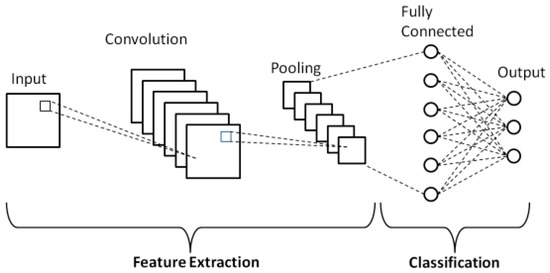
\includegraphics[width=0.5\textwidth]{cnn_model}
		\caption{Schematic diagram of a basic convolutional neural network (CNN) architecture\cite{phung}}
	\end{figure}
	\FloatBarrier
	\paragraph~	Deep learning techniques have emerged recently and advances in convolutional neural networks (CNN) surpass the classical approach to hand gesture recognition as it eliminates the need to derive complex handcrafted features from images\cite{gesturecnn}. CNN's automate the feature extraction process by learning high-level abstractions in images and capturing the most distinguishing feature values using the hierarchical architecture. Thus, it solves the disadvantage of obtaining inconsistent property descriptors when working with large numbers of motion classes with very small cross-class variations\cite{static}.
	
	\section{Model Architecture for LE-NET5}
	\paragraph~ LeNet-5 was one of the earliest convolutional neural networks to support the deep learning event. After countless years of analysis and numerous compelling iterations, the final result was named LeNet-5 in 1988.
	
	\begin{figure}[h!]
		\centering
		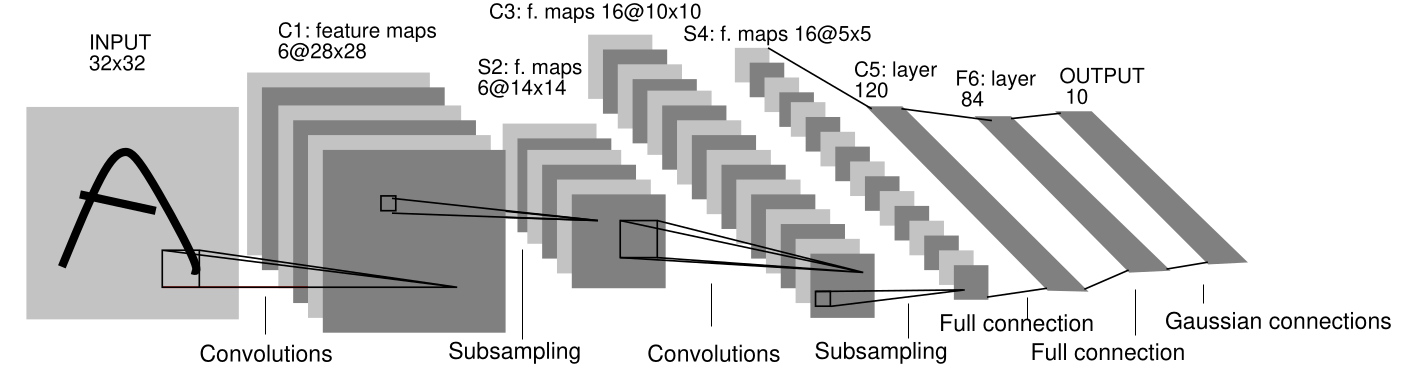
\includegraphics[width=1\textwidth]{lenet}
		\caption{Architecture of LeNet-5, a Convolutional Neural Network, here for digits recognition. Each plane is a feature map, i.e. a set of units
			whose weights are constrained to be identical.\cite{lenet}}
	\end{figure}
	\FloatBarrier
	
	\paragraph~ LeNet-5 A total of seven layers, each with no input with trainable parameters; each layer has multiple FeatureMap, which is a property of each of the FeatureMap inputs extracted via a convolution filter, and then each FeatureMap has multiple neurons.\\
	
	\textbf{C1 layer-convolutional layer:}\\
	\paragraph~ The first convolution operation is performed on the input image (using 6 convolution kernels of size 5*5) to obtain 6 feature maps of C1 (6 feature maps of size 28 28, 32-5 + 1 = 28). The size of the convolution kernel is 5, and there are 6 (5 * 5 + 1) = 156 parameters in total, where +1 indicates that a kernel has a bias. For convolution layer C1, each pixel in C1 is dependent on 5 of 5 pixels and 1 aberration in the input image, so there are 156 28 * 28 = 122304 links in total.\cite{lenet}\\
	
	\textbf{S2 layer-pooling layer (downsampling layer):}\\
	\paragraph~ The pooling is done immediately after the first convolution. Pooling is done using 2 cores and S2, 14x14 (28/2 = 14) 6 feature maps are obtained. S2's pooling layer is a weighting coefficient plus an offset multiplied by the sum of the pixels in the 2*2 area in C1, and then the result is remapped. So each pooling core has two training parameters i.e. 2x6 = 12 training parameters but there are 5x14x14x6 = 5880 connections.\cite{lenet}\\
	
	\textbf{C3 layer-convolutional layer:}\\
	\paragraph~ After the first pooling, the second convolution, the output of the second convolution is C3, 16 pieces of 10x10 feature maps, and the size of the convolution kernel is 5. The first 6 feature maps of C3 (corresponding to column 6 of the first). red box) connects to 3 feature maps connected to S2 layer and next 6 feature maps are connected to S2 layer 4 feature maps are connected, next 3 feature maps are connected to 4 feature maps are unconnected in S2 layer and last one is linked to all feature maps in S2 layer. The convolution kernel size is still 5x5, so there are 6 (3*5*5 + 1) + 6 (4*5*5 + 1) + 3 (4*5*5 + 1) +1 (6*5*5 + 1) = 1516 parameters. The image size is 10 10 so there are 151600 connections.\cite{lenet}\\
	
	\textbf{S4 layer-pooling layer (downsampling layer):}\\
	\paragraph~ S4 is the pooling layer, the window size is still 2*2, a total of 16 feature maps and 16 10x10 maps of the C3 layer are pooled in units of 2x2 to get 16 5x5 feature maps. This layer has a total of 32 training parameters, 2x16, 5x5x5x16 = 2000 connections.\cite{lenet}\\
	
	\textbf{C5 layer-convolution layer:}\\
	\paragraph~ The C5 layer is a convolution layer. Since the size of the 16 images of the S4 layer is 5x5, the size of the image formed after convolution is 1x1, which is the same as the size of the convolution kernel. This results in 120 convolution results. Each is linked to 16 maps from the previous level. So there are (5x5x16 + 1) x120 = 48120 parameters and there are also 48120 connections.\cite{lenet}\\
	
	\textbf{F6 layer-fully connected layer:}\\
	\paragraph~ Layer 6 is a fully connected layer. The F6 layer has 84 nodes corresponding to a 7x12 bitmap, -1 means white, 1 means black, so the black and white of each symbol's bitmap corresponds to a code. The training parameters and number of connections for this layer is (120 + 1) x84 = 10164.\cite{lenet}\\
	\section{Python Libraries for Project}
	
	\subsection{Python-Peripherial}
	\paragraph~ Python-periphery is a pure Python library for GPIO, LED, PWM, SPI, I2C, MMIO, and Serial peripheral I/O interface access in userspace Linux. Useful in embedded Linux environments (including Raspberry Pi) for interfacing with external peripherals.\cite{perip}
	\subsection{Tensorflow-Keras}
	\paragraph~ TensorFlow 2 is an end-to-end, open-source machine learning platform.\cite{tensorflow} It enables it to efficiently execute low-level tensor operations on the CPU, GPU, or TPU. Calculates the gradient of arbitrarily differentiable expressions.\cite{tensorflow} Scales computation to many devices, such as clusters of hundreds of GPUs.\cite{tensorflow} Streams programs ("graphics") to external runtimes such as servers, browsers, mobile, and embedded devices.\cite{tensorflow} It combines these four key features in one platform.\cite{keras}
	\chapter{MATERIALS AND METHODS}
	\section{Htpa32x32d Thermopile Infrared Array}
	\paragraph~ The sensor chosen to be used in the project is HTPA32x32d thermopile array sensor.
	HTPA32x32d thermopile array sensor 32x32 pixel, operates between -10 and 70 degrees,
	provides I2C communication, has an internal EEPROM and provides an 8-bit data set.
	EEPROM data contains calibration data for each pixel of the sensor.\\
	
	\begin{figure}[h!]
		\centering
		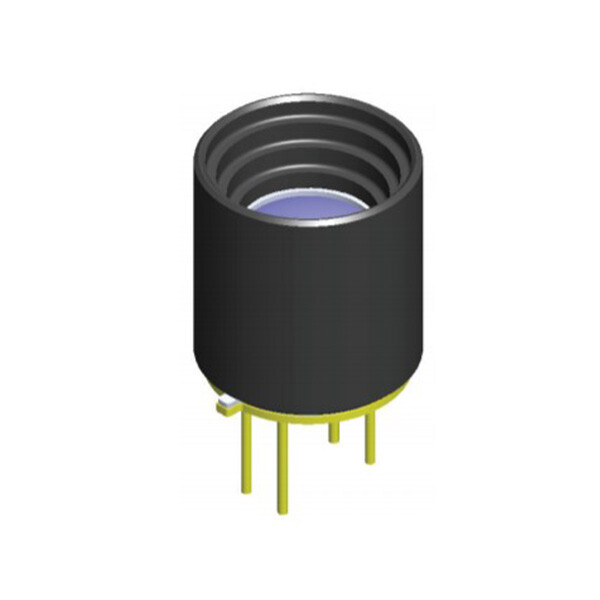
\includegraphics[width=0.35\textwidth]{htpa}
		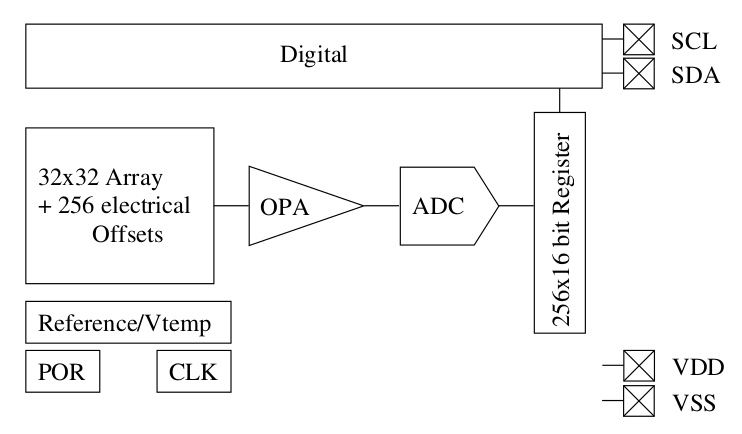
\includegraphics[width=0.5\textwidth]{htpasema}
		\caption{Schematic for HTPA32x32d}
	\end{figure}
	\FloatBarrier
	\begin{flushleft}
		\begin{table}[h!]
			
			\caption{Genaral Features HTPA32x32d}
			
			
			\begin{tabular}{|l|l|l|l|l|}
				\hline
				Features\textbackslash\{\}& Sensitivity & Therm. Pix. Time Const. & Digital Interface & EEPROM Size\\\hline
				& 450V/W&$<4ms $& I2C & 64kBit  \\\hline
				Features\textbackslash\{\}& Max Frame&Field of View & Selectable Clock & Storage Temperature \\\hline
				&60 Hz& 33*33 deg & 1 to 13 Mhz & -40/85 Deg.C \\\hline
			\end{tabular}
		\end{table}
	\end{flushleft}
	\FloatBarrier
	\section{Sensor and MCU Communication PCB Design}
	\paragraph~ A mini card has been designed between the sensor and the Raspberry pi card to communicate. However, the card could not be printed. The card that will connect the sensor and the motherboard has been designed completely according to the standards recommended by Heimann company.\\
	\begin{figure}[h!]
		\centering
		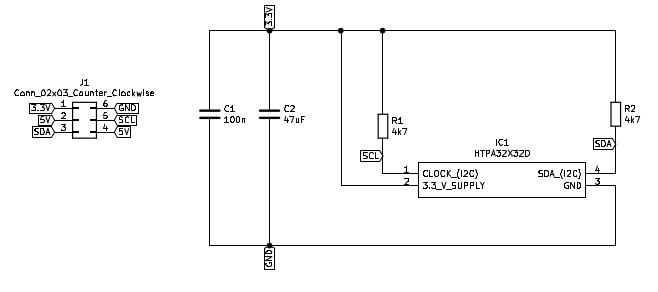
\includegraphics[width=0.6\textwidth]{schematic}
		\caption{Schematic Design of Communication PCB}
		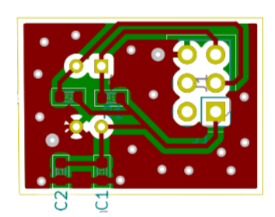
\includegraphics[width=0.4\textwidth]{pcb}
		\caption{PCB Design of Communication PCB}
	\end{figure}
	\FloatBarrier
	\paragraph~ In addition to this, we have produced a product suitable for a schematic on a mini perforated plate for use in communication with the card. In addition, we designed a protective cage from a 3d printer to protect the sensor.\\
	\begin{figure}[h!]
		\centering
		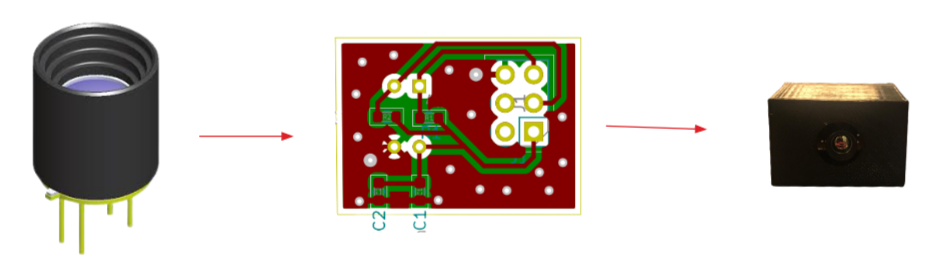
\includegraphics[width=1\textwidth]{mb}
		\caption{Mini Sensor Board}
	\end{figure}
	
	\section{Dataset}
	\subsection{Multi-Modal Hand Gesture Dataset for Hand Gesture Recognition}
	\paragraph~ This dataset was created to validate a hand-gesture recognition system for Human-Machine Interaction (HMI). It is composed of 15 different hand-gestures (4 dynamic and 11 static) that are split into 16 different hand-poses, acquired by the Leap Motion device. Hand-gestures were performed by 25 different subjects (8 women and 17 men). Every gesture has 20 instances (repetitions) per subject, performed in different locations in the image.\cite{dataset}\\
	for static and dynamic gestures:\\
	This set contains 16 hand-poses, used for both static and dynamic hand-gestures:\\
	A: L
	B: fist moved
	C: index
	D: ok
	E: C
	F: heavy
	G: hang
	H: two
	I: three
	J: four
	K: five
	L: palm
	M: down
	N: palm moved
	O: palm up
	P: up
	\begin{figure}[h!]
		\centering
		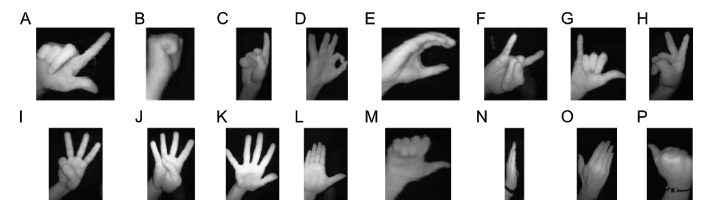
\includegraphics[width=0.8\textwidth]{data1.png}
		\caption{Hand Gesture Dataset}
	\end{figure}
	\FloatBarrier
	\section{Data Augmentation}
	\paragraph~ Using this dataset, a new train and validation set was created for the static gestures in the project. A total of 36800 and 9200 train and validation sets were created with randomly selected images.However, both resizing and data augmentation were done in order to make the data set suitable for the project.\cite{aug}
	
	\begin{figure}[h!]
		\centering
		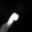
\includegraphics[width=0.2\textwidth]{close_test289}
		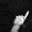
\includegraphics[width=0.2\textwidth]{index_test179}
		
\includegraphics[width=0.2\textwidth]{last_test71}
		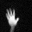
\includegraphics[width=0.2\textwidth]{open_test_0_9826}
		\caption{Close-Index-Last Page-Open Gestures}
	\end{figure}
	\FloatBarrier
	
	\chapter{PROGRESS AND RESULT}
	\paragraph~ In this section, the methods to be applied in the project are included.
	
	\begin{figure}[h!]
		\centering
		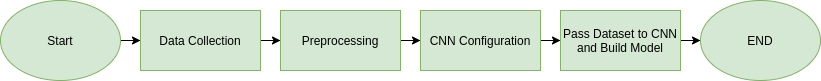
\includegraphics[width=1\textwidth]{framework}
		\caption{System Framework for Static Gestures}
	\end{figure}
	\FloatBarrier
	
	\section{Capture Thermopiles Image}
	\subsection{Heimann Thermopile Array Sensor communication}
	\paragraph~ First, I provided the connections between the sensor and the Raspberry Pi in order to receive the image. I provided the communication with the mini card I made in section 4.2 using the I2C protocol.
	
	\paragraph~ With the device connected to a Raspberry Pi, and with the Pi configured.\cite{adaf} correctly for I2C, I was able to see the devices connected with the i2cdetect command.
	\begin{figure}[h!]
		\centering
		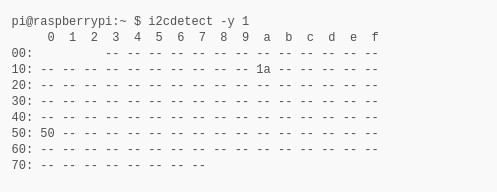
\includegraphics[width=0.8\textwidth]{raspi1.png}
		\caption{Thermopile Infrared Array Device and EEPROM Addresses}
	\end{figure}
	\FloatBarrier
	
	\paragraph~ In order to be able to read the data properly, the python-periphery\cite{perip} library was used. The sensor is divided into two parts (Top and Bottom Half), which are also divided into 4 blocks. The reading order is shown below for different blocks. When a conversion is initiated, the X Block of the upper and lower half are measured simultaneously. Each block consists of 128 Pixels sampled entirely in parallel. The reading order in the lower half is mirrored compared to the upper half so the center lines are always read last.
	
	\begin{table}[h!]
		\begin{center}
			\caption{Read Data 1 Command (Top Half of Array)}
			\begin{tabular}{|c|c|c|c|c|c|c|c|c|} 
				\hline
				Addr/CMD & \multicolumn{8}{c|}{0x1A (7 Bit!) / 0x0A}\\\cline{1-9}
				Read Data &7&6&5&4&3&2&1&0\\
				\cline{1-9}
				1. Byte / 2. Byte & \multicolumn{8}{c|}{PTAT 1 MSB / LSB or Vdd 1 MSB / LSB}\\\cline{1-9}
				3. Byte / 4. Byte & \multicolumn{8}{c|}{Pixel (0+BLOCK*128) MSB / LSB}\\\cline{1-9}
				5. Byte / 6. Byte & \multicolumn{8}{c|}{Pixel (1+BLOCK*128) MSB / LSB}\\\cline{1-9}
				... & \multicolumn{8}{c|}{}\\\cline{1-9}	
				257. Byte / 258. Byte & \multicolumn{8}{c|}{Pixel (127+BLOCK*128) MSB / LSB}\\\cline{1-9}
				
			\end{tabular}
		\end{center}
	\end{table}
	\FloatBarrier
	\begin{table}[h!]
		\begin{center}
			\caption{Read Data 2 Command (Bottom Half of Array)}
			\begin{tabular}{|c|c|c|c|c|c|c|c|c|} 
				\hline
				Addr/CMD & \multicolumn{8}{c|}{0x1A (7 Bit!) / 0x0B}\\\cline{1-9}
				Read Data &7&6&5&4&3&2&1&0\\
				\cline{1-9}
				1. Byte / 2. Byte & \multicolumn{8}{c|}{PTAT 2 MSB / LSB or Vdd 2 MSB / LSB}\\\cline{1-9}
				3. Byte / 4. Byte & \multicolumn{8}{c|}{Pixel (992-BLOCK*128) MSB / LSB}\\\cline{1-9}
				5. Byte / 6. Byte & \multicolumn{8}{c|}{Pixel (993-BLOCK*128) MSB / LSB}\\\cline{1-9}
				... & \multicolumn{8}{c|}{}\\\cline{1-9}	
				65. Byte / 66. Byte & \multicolumn{8}{c|}{Pixel (1023-BLOCK*128) MSB / LSB}\\\cline{1-9}
				
				65. Byte / 66. Byte & \multicolumn{8}{c|}{Pixel (1023-BLOCK*128) MSB / LSB}\\\cline{1-9}
				
				67. Byte / 68. Byte & \multicolumn{8}{c|}{Pixel (960-BLOCK*128) MSB / LSB}\\\cline{1-9}
				
				69. Byte / 70. Byte & \multicolumn{8}{c|}{Pixel (961-BLOCK*128) MSB / LSB}\\\cline{1-9}
				
				... & \multicolumn{8}{c|}{}\\\cline{1-9}
				
				129. Byte / 130. Byte & \multicolumn{8}{c|}{Pixel (991-BLOCK*128) MSB / LSB}\\\cline{1-9}
				
				131. Byte / 132. Byte & \multicolumn{8}{c|}{Pixel (928-BLOCK*128) MSB / LSB}\\\cline{1-9}
				
				...& \multicolumn{8}{c|}{}\\\cline{1-9}
				
				257. Byte / 258. Bytes& \multicolumn{8}{c|}{Pixel (927-BLOCK*128) MSB / LSB}\\\cline{1-9}
				
			\end{tabular}
		\end{center}
	\end{table}
	\FloatBarrier
	Each block is checked before it is read. The python-opencv\cite{cv2} library was used to visualize the obtained result.
	\begin{figure}[h!]
		\centering
		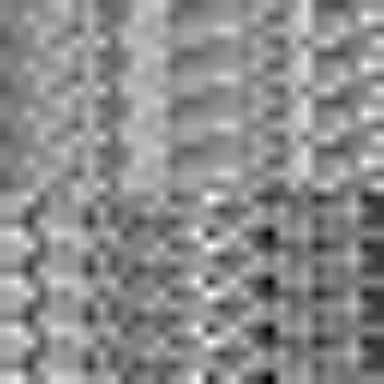
\includegraphics[width=0.23\textwidth]{4.img}
		
\includegraphics[width=0.23\textwidth]{3.img}
		\caption{Thermal Image}
	\end{figure}
	\FloatBarrier
	
	
	\paragraph~ Each pixel (or each analog-to-digital converter, given the repeating structure corresponding to each "block" of the sensor) has its own offset and sensitivity to incident light. Without calibrating it, this constant "noise" suppresses the signal from changing IR/temperature conditions. By subtracting the two frames in quick succession, this common noise signal is removed.
	
	\paragraph~ However, it is still quite noisy, as this frame subtraction increases random noise (since we now have contributions from two frames) and does not correct pixel-dependent sensitivity.
	Only fabrication calibration will be done with EEPROM data in the next step.
	\subsection{Calibrating images from Heimann Thermopile Array Sensor}
	
	\paragraph~ After reading an image off a Heimann thermopile array, the pixel values can be converted to temperature readings through the use of calibration parameters stored on the device. To extract the calibration parameters, it is easiest to first read off the entire EEPROM on the thermopile array.
	
	\begin{figure}[h!]
		\centering
		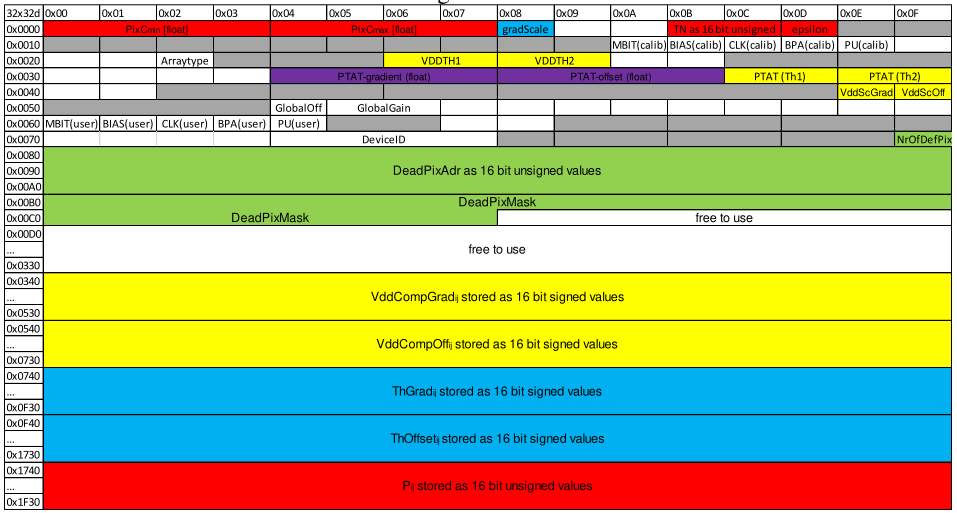
\includegraphics[width=1\textwidth]{eeprom}
		\caption{EEPROM overview 32x32d\cite{datasheet}}
	\end{figure}
	\FloatBarrier
	\paragraph~ Then, parameters and calibration values can be extracted from this array, as described in the Heimann datasheet.\cite{datasheet}\\
	Calibration for only one pixel is done as follows.\\
	$PTAT_{av} = \frac{\sum \limits _{i=0}^{7}{PTAT_i}}{8}=38152 Digits $ \\
	$PTAT_{gradient}=0.0211 dK/Digit $ and $PTAT_{offset}=2195.0dK$ \\
	$ V_{00}=34435 Digits $\\
	$ elOffset[0]=34240 $\\
	$gradScale=24  $\\
	$ThGrad_{00}=11137$ \\
	$ThOffset_{00}=65506 $\\
	$VDD_{av}=35000 $\\
	$ VDD_{TH1}= 33942 $\\
	$ VDD_{TH2} = 36942 $\\
	$ PTAT_{TH1} = 30000  $\\
	$ PTAT_{TH_2} = 42000  $\\
	$ VddCompGrad[ 0 ] = 10356 $\\
	$ VddCompOff[ 0 ] =51390  $\\
	$ VddScGrad = 16 $\\
	$VddScOff = 23  $\\
	$ PixC_{00}= 1\cdot087\cdot10^8 $\\
	$ PCSCALEVAL = 1\cdot10^8 $\\
	Calculation of ambient temperature:\\
	$ 	T_a=PTAT_{av} \cdot PTAT_{gradient}+ PTAT_{offset}=38152 \cdot 0.0211 + 2195.0 dK =3000 dK $\\
	Compensation of thermal offset:\\
	$V_{00\_Comp}=V_{00}-\frac{Th_{Grad00} \cdot T_a}{2^{gradScale}}-Th_{Offset_{00}}=34439 $\\
	Compensation of electrical offset:\\
	$ 	V_{00\_Comp}^{\ast} =V_{00\_Comp}-elOffset[0]=199 $\\
	Compensation of supply voltage:\\
	$ V_{00-VDD_{Comp}}=V_{00\_Comp}^{\ast}-\frac{\frac{Vdd_{CompGrad}[0]\cdot PTAT_{av}}{2^{Vdd_{ScGrad}}}+V_{Vdd_{Compoff}}[0]}{2^{Vdd_{ScOff}}}\\
	\cdot(VDD_{av}-VDD_{TH1}-(\frac{VDD_{TH2}-VDD_{TH1}}{PTAT_{TH2}-PTAT_{TH1}})\cdot(PTAT_{av}-PTAT_{TH1}))=199-1=198 $
	The sensitivity coefficients ( PixC ij ) are calculated:\\
	$PixC_{00}=(\dfrac{P_{00} \cdot (PixC_{Max}-PixC_{Min})}{65535}+PixC_{Min}) \cdot \frac{epsilon}{100} \cdot \frac{GlobalGain}{100000}=1\cdot087\cdot10^8 $\\
	Leading to a compensation of the pixel voltage:\\
	$V_{00PixC}=\dfrac{	V_{00-VDD_{Comp}}\cdot PCSCALEVAL}{PixC_{0}}=182$\\ 
	
	All operations are applied for 1024 pixels. Application result images are as in figure 4.4.
	
	\begin{figure}[h!]
		\centering
		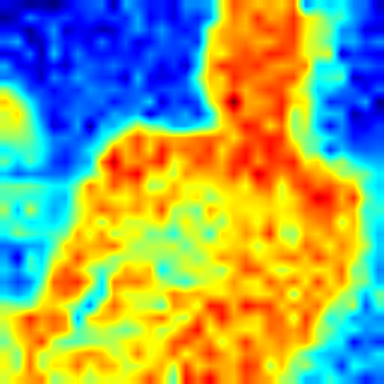
\includegraphics[width=0.23\textwidth]{last_test58}
		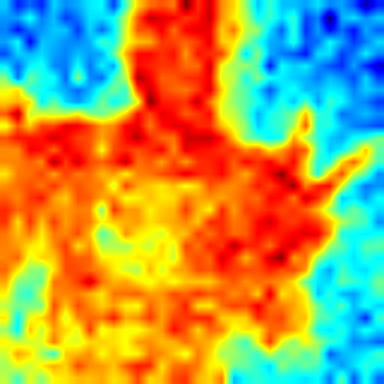
\includegraphics[width=0.23\textwidth]{last_test59}
		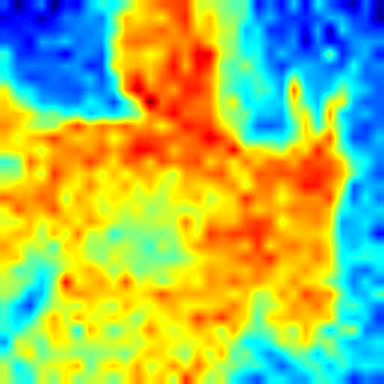
\includegraphics[width=0.23\textwidth]{last_test60}
		\caption{Thermal Images with EEPROM Calibration Data}
	\end{figure}
	\FloatBarrier
	\paragraph~	\textbf{NOTE:All steps to acquired the image are made with reference to the datasheet\cite{datasheet}.}
	\section{Hand Thermal Image Isolation}
	\paragraph~ The hand was isolated from the background without using any image processing method. For this, it has been arranged in a way that can remove the ambient temperature of the device from the image before giving a command. First, the average of 10 images was taken and given to all images. Thus, the background temperature was isolated.
	\begin{figure}[h!]
		\centering
		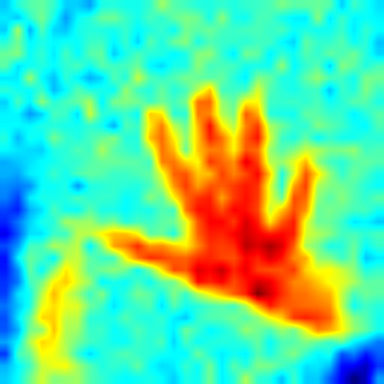
\includegraphics[width=0.23\textwidth]{rgb0}
		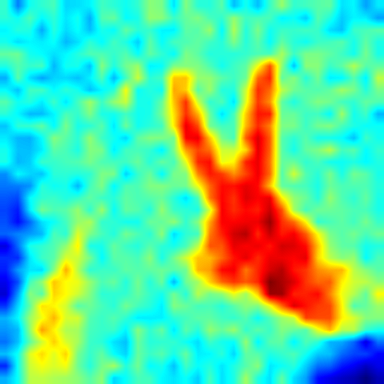
\includegraphics[width=0.23\textwidth]{rgb1}
		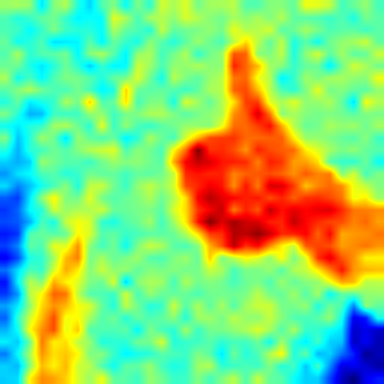
\includegraphics[width=0.23\textwidth]{rgb2}
		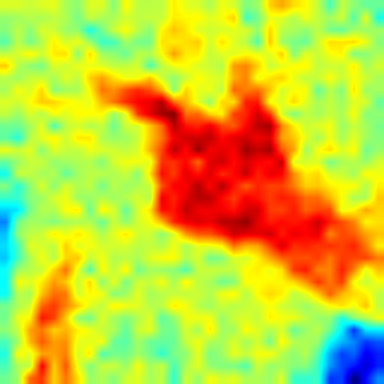
\includegraphics[width=0.23\textwidth]{rgb3}
		\caption{Thermal Images with Background}
	\end{figure}
	
	\section{Hand Gesture Recognition}
	\subsection{Static Gesture Recognition}
	
	
	\paragraph~	A number of scenarios have been prepared for command matching for the smart mirror. The scenarios prepared are as follows;
	
	\paragraph~	For Static Movements:
	
	\paragraph~	There are 4 fixed movements. It is the ability to Open, Close, Tap and Return to Home.
	
	\begin{figure}[h!]
		\centering
		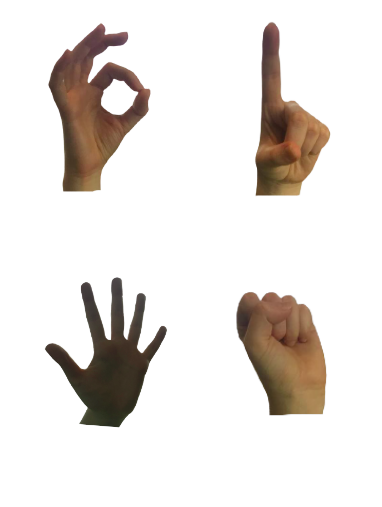
\includegraphics[width=0.27\textwidth]{tek2}
		\caption{Gestures of Open,Close,Touch,Return to the Home Page }
	\end{figure}
	\FloatBarrier
	\paragraph~ We tried to create our own data set using the data set we mentioned in Section 3.3. We used images that are similar to each of the four identified gestures. It was found correct to use K: Five set for Open, B: First Moved set for Close, C: Index set for Touch, A:L set for ,Return to the Home Page.\cite{dataset} First, the images were cropped and resized that are chosen mixed. After these processes, the data reproduced by data augmentation were divided into two as validation and training data. The number of trains defined for each movement is approximately 9200, and the number of validation images is around 2300.
	
	\subsubsection{Model Architecture for LE-NET5}
	\paragraph~ In 1989, Yann LeCun presented a convolutional neural network called LeNet. Generally, LeNet refers to LeNet-5 and is a simple convolutional neural network.\cite{lenet}
	
	\paragraph~The fact that our Input Image sizes are 32X32 was the biggest factor pushing us to use this model. Since we could not use a ready dataset, the change in the number of layers in order to train our model well, resulted in good results.
	
	\begin{figure}[h!]
		\centering
		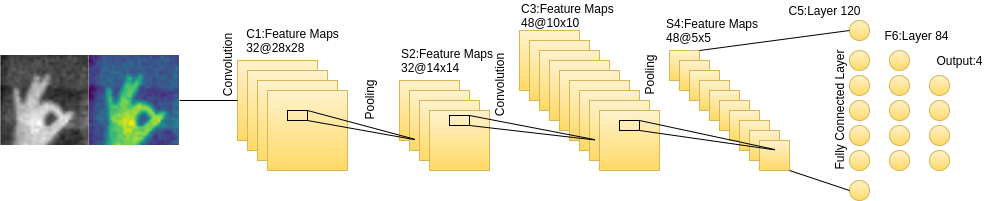
\includegraphics[width=1\textwidth]{cnn}
		\caption{A~ Structural Diagram of the Proposed LENET5 for Static Gesture}
	\end{figure}
	\FloatBarrier
	\paragraph~ The general architecture for LeNet-5 is as given in Figure 3. The input layer C1 acts like the retina, which receives centered and size-normalized gesture images (otherwise, some images may not fit in the input layer). The next layer, S2, consists of several feature maps that have the same role to gestures as their simple cells. In practice, a feature map is a square. The weights in a feature map need to be the same so they can detect the same local feature in the input image. The weights between feature maps are different so they can detect different local features. Each unit in a feature map has a receiver field.
	
	\begin{table}[h!]
		\begin{center}
			\caption{The structural layers and number of parameters of the
				LENET5.}
			\begin{tabular}{|l|l|l|}
				\hline
				\multicolumn{3}{|c|}{Model:"Static\_Gesture\_Model} \\
				\hline
				Layer(type) & Output Shape & Param\# \\
				\hline
				conv2d\_8 (Conv2D)   & (None, 28, 28, 32)  & 832 \\
				\hline
				max\_pooling2d\_8 (MaxPooling2) & (None, 14, 14, 32)   &  0 \\
				\hline
				conv2d\_9 (Conv2D)   &  (None, 10, 10, 48)    &   38448   \\
				\hline
				max\_pooling2d\_9 (MaxPooling2) & (None, 5, 5, 48)      &  0 \\
				\hline
				flatten\_4 (Flatten)  & (None, 1200)   & 0 \\
				\hline
				dense\_16 (Dense) & (None,120)  & 307456 \\
				\hline
				dense\_17 (Dense) & (None, 84) &   21588  \\
				\hline
				dense\_18 (Dense) & (None, 10) &   850  \\
				\hline
				dense\_19 (Dense)  &   (None, 4)       &   44  \\
				\hline
				\multicolumn{3}{|l|}{Total params: 369,218} \\
				\multicolumn{3}{|l|}{Trainable params: 369,218} \\
				\multicolumn{3}{|l|}{Non-trainable params: 0}\\
				\hline
			\end{tabular}
		\end{center}
	\end{table}
	\FloatBarrier
	\paragraph~ If to summarize the model we outlined in the table, we use two convolutional layers, then twice a pooling layer (32-filters and 48-filters, respectively), and finally three fully connected layers with 4-class softmax units.
	
	\FloatBarrier
	\begin{figure}[h!]
		\centering
		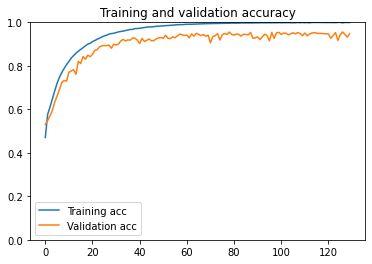
\includegraphics[width=0.4\textwidth]{learning_8_0}
		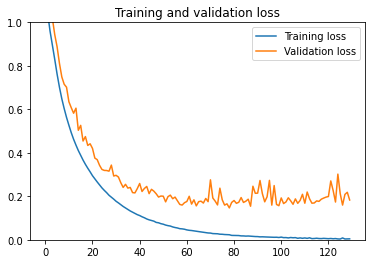
\includegraphics[width=0.4\textwidth]{learning_9_0}
		\caption{Loss and Accuracy Curves (Training and Validation Set)}
	\end{figure}
	\FloatBarrier
	\paragraph~ And the result is close to perfect. Data augmentations worked. The learning algorithm, which reached 95\% validation accuracy, gave very successful results. In the next step, images will be given to the model again for testing and the results will be observed.
	\subsubsection{Test Sets and Results}
	\subsection{Dynamic Gesture Recognition}
	
	\begin{table}[h!]
		\begin{center}
			\caption{Trim Register 1 (write only)\cite{datasheet}}
			\begin{tabular}{|c|c|c|c|c|c|c|c|c|}
				\hline
				Addr / CMD & \multicolumn{8}{c|}{0x1A (7 Bit!) / 0x03} \\
				\hline
				Trim Reg 1 & 7 & 6 &5  &4  &3  &2  &1&0  \\
				\hline
				Name & \multicolumn{2}{c|}{RFU} & \multicolumn{2}{c|}{REF\_CAL}& \multicolumn{4}{c|}{MBIT TRIM}\\
				\hline
			\end{tabular}
		\end{center}
	\end{table}
	\FloatBarrier
	
	REF\_CAL: selectable amplification
	\\
	
	MBIT\_TRIM: m = 4 to 12 (m+4) bit as ADC resolution\\
	
	\paragraph~ In order to get the maximum efficiency from the sensor, to set the ADC Resolution to 16 bits, m of 12 was determined according to the data in the table. Since the framerate was too low, it was decided to speed up by sacrificing quality, but the quality was too low, revealing that ADC resolution should not be compromised. According to the resolutions, the images are as in figure 2.\\
	\begin{figure}[h!]
		\centering
		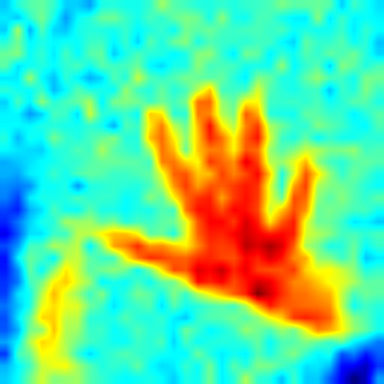
\includegraphics[width=0.23\textwidth]{rgb0}
		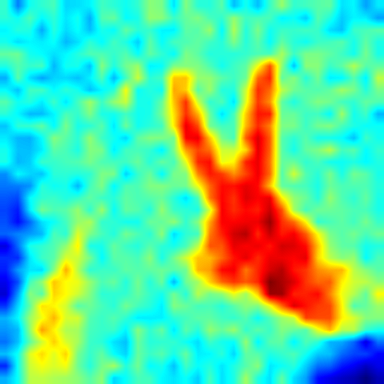
\includegraphics[width=0.23\textwidth]{rgb1}
		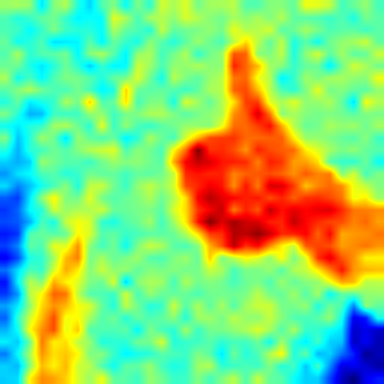
\includegraphics[width=0.23\textwidth]{rgb2}
		\caption{Thermal Images 8Bit-12Bit-16Bit ADC Resolution)}
	\end{figure}
	\begin{table}[h!]
		\begin{center}
			\caption{Trim Register 2 (write only)\cite{datasheet}}
			\begin{tabular}{|c|c|c|c|c|c|c|c|c|}
				\hline
				Addr / CMD & \multicolumn{8}{c|}{0x1A (7 Bit!) / 0x04} \\
				\hline
				Trim Reg 1 & 7 & 6 &5  &4  &3  &2  &1&0  \\
				\hline
				Name & \multicolumn{3}{c|}{RFU} & \multicolumn{5}{c|}{BIAS TRIM TOP}\\
				\hline
			\end{tabular}
		\end{center}
	\end{table}
	\FloatBarrier
	BIAS\_TRIM\_TOP:0 to 31 $ \longrightarrow $ $ 1\mu A $ to $ 13 \mu A $\\
	
	\begin{table}[h!]
		\begin{center}
			\caption{Trim Register 3 (write only)\cite{datasheet}}
			\begin{tabular}{|c|c|c|c|c|c|c|c|c|}
				\hline
				Addr / CMD & \multicolumn{8}{c|}{0x1A (7 Bit!) / 0x05} \\
				\hline
				Trim Reg 1 & 7 & 6 &5  &4  &3  &2  &1&0  \\
				\hline
				Name & \multicolumn{3}{c|}{RFU} & \multicolumn{5}{c|}{BIAS TRIM BOT}\\
				\hline
			\end{tabular}
		\end{center}
	\end{table}
	\FloatBarrier
	BIAS\_TRIM\_BOT: 0 to 31 $ \longrightarrow $ $ 1\mu A $ to $ 13 \mu A $\\
	\paragraph~ This setting is used to adjust the bias current of the ADC. A faster clock frequency requires a
	higher bias current setting.\cite{datasheet}\\
	
	\paragraph~ Having ADC resolution 16 made us think that it did not affect us much. Afterward, it was said that if the BIAS current value is set to the maximum, its speed may increase. However, as a result of this experiment, almost no change was observed in the framerate.\\
	
	\begin{table}[h!]
		\begin{center}
			\caption{Trim Register 4 (write only)\cite{datasheet}}
			\begin{tabular}{|c|c|c|c|c|c|c|c|c|}
				\hline
				Addr / CMD & \multicolumn{8}{c|}{0x1A (7 Bit!) / 0x06} \\
				\hline
				Trim Reg 1 & 7 & 6 &5  &4  &3  &2  &1&0  \\
				\hline
				Name & \multicolumn{2}{c|}{RFU} & \multicolumn{6}{c|}{CLK TRIM}\\
				\hline
			\end{tabular}
		\end{center}
	\end{table}
	\FloatBarrier
	CLK\_TRIM:0 to 63 $ \longrightarrow $ $ 1 MHz $ to $ 13 MHz $\\
	
	\paragraph~ The point where we could most easily observe the increase in Frame Rate was the Clock Trim set. Although I set the maximum value, I could not get the desired result here.\\
	\section{Matching Gesture to Commands of Smart Mirror}
	
	\paragraph~ In the project carried out by Vestel, friends who are interested in the smart mirror part are expected to define the gestures for the android side of the smart mirror.
	\newpage
	\chapter{Work Plan and Work Packages}
	\begin{landscape}
		\noindent\resizebox{260mm}{!}{\begin{ganttchart}[
				hgrid style/.style={black, dotted},
				vgrid={*5{black,dotted}, *1{white, dotted}, *1{black, dashed}},
				x unit=2mm,
				y unit chart=9mm,
				y unit title=12mm,
				time slot format=isodate,
				group label font=\bfseries \Huge,
				link/.style={->, thick}
				]{2020-10-01}{2021-04-16}
				\gantttitlecalendar{year, month=name, week}\\
				
				\ganttgroup[
				group/.append style={fill=orange}
				]{Literature Review and Material Supply}{2020-10-01}{2021-01-15}\\ [grid]
				\ganttorangebar[
				name=Documentation
				]{Literature Review}{2020-10-01}{2021-01-15}\\ [grid]
				\ganttorangebar[
				name=FMETutorial
				]{Material Supply}{2020-12-01}{2021-01-15}\\ [grid]
				%%%%%%%%%%WP2%%%%%%%%%%%%
				\ganttgroup[
				group/.append style={fill=blue}
				]{Sensor PCB Design}{2021-01-11}{2021-02-03}\\ [grid]
				
				\ganttbluebar[
				name=FMETutorial
				]{Referance Circuit Rewiev}{2021-01-11}{2021-01-13}\\ [grid]
				\ganttlinkedblackbar{}{2021-01-13}{2021-01-14}
				\ganttbluebar[
				name=FMETutorial
				]{Schematic Design}{2021-01-14}{2021-01-15}\\ [grid]
				
				\ganttlinkedblackbar{}{2021-01-15}{2021-01-16}
				\ganttbluebar[
				name=FMETutorial
				]{PCB Design}{2021-01-16}{2021-01-18}\\ [grid]
				
				\ganttlinkedbluebar{}{2021-01-18}{2021-02-01}
				
				\ganttbluebar[
				name=FMETutorial
				]{Testing Sensor PCB}{2021-02-01}{2021-02-03}\\ [grid]
				%%%%%%%%%%%%%%%%%%%WP3%%%%%%%%%%%%%%%%%%%%%%%%%%%%%%
				\ganttgroup[
				group/.append style={fill=red}
				]{Gesture Detection}{2021-01-03}{2021-04-15}\\ [grid]
				%\ganttredbar[
				%name=FMETutorial
				%]{Hand Thermal Image Isolation}{2020-01-03}{2021-01-21}\\ [grid]
				\ganttredbar[
				name=FMETutorial
				]{Receiving Data From The Sensor}{2021-01-03}{2021-01-05}\\ [grid]
				\ganttlinkedblackbar{}{2021-01-05}{2021-01-06}
				\ganttredbar[
				name=FMETutorial
				]{Making The Data Meaningful}{2021-01-06}{2021-01-07}\\ [grid]
				\ganttlinkedblackbar{}{2021-01-07}{2021-01-08}
				\ganttredbar[
				name=FMETutorial
				]{Isolation of The Hand From The Data Received From the Sensor}{2021-01-08}{2021-01-18}\\ [grid]
				\ganttlinkedblackbar{}{2021-01-18}{2021-01-19}
				\ganttredbar[
				name=FMETutorial
				]{Detecting Hand Condition}{2021-01-19}{2021-01-30}\\ [grid]
				\ganttlinkedblackbar{}{2021-01-30}{2021-02-01}
				\ganttredbar[
				name=FMETutorial
				]{ Creating Dataset for Static Gesture }{2021-02-01}{2021-02-15}\\ [grid]
				\ganttlinkedblackbar{}{2021-02-15}{2021-02-16}
				\ganttredbar[
				name=FMETutorial
				]{Creating LENET-5 Model for Static Gesture }{2021-02-16}{2021-03-15}\\ [grid]
				\ganttlinkedblackbar{}{2021-03-15}{2021-03-16}
				\ganttredbar[
				name=FMETutorial
				]{Testing LENET-5 Model for Static Gesture }{2021-03-16}{2021-04-15}\\ [grid]
		\end{ganttchart}}
	\end{landscape}
	\newpage
	\chapter{COST ANALYSIS}
	\section{Economical Costs}
	
	\paragraph~	In this project, the economic cost is only in the hardware part. A Raspberry Pi 4B and Thermopil array sensor are used in our project. The market price of Raspberry Pi 4B is \$55. The thermopil array sensor, on the other hand, has been chosen the most suitable for our project and has been researched for the market. The price of the HEIMANN HTPA32x32d Thermopil array sensor is \$87. There is currently no separate cost in the software part. Because using opensource software.
	
	\section{Environmental,Political and Social Costs}
	\paragraph~	Infrared sensor arrays have emerged in recent years and are products that allow the application of thermal imaging technologies to consumer electronics. With the introduction of Covid-19 into our lives, it is frequently encountered in the field of thermal imaging. Since a consumer electronics product using these products has not been produced in Turkey yet, it is considered to contribute to the national knowledge. In the project where privacy is prioritized, the privacy of the person will be ensured by using a thermopile array sensor. Also, the project is executed by Vestel A.Ş. so the project is expected to inspire different projects within Vestel. The fact that these sensors are newly introduced to the market will pave the way for innovative applications in many fields and thus method changes that can turn into patents. For example, although gesture recognition is performed with cameras conventionally, it offers a significant innovation in methodology, using passive infrared arrays. Smart mirrors that can be controlled with gesture recognition can have a positive effect on the preference of the products in question by the consumers. In doing so, using a technology that does not impair personal privacy will ensure that the users put the product into their lives safely and the applications related to the product become widespread.
	
	\chapter{CONCLUSION}
	
	\newpage
	\bibliographystyle{deueeebst2.bst}
	
	\bibliography{fp_refs}
	\newpage
	\chapter{APPENDIX}
	
	%

    
    \hypertarget{sensor-configuration}{%
\section{\textbf{Sensor Configuration}}{Sensor Configuration}\label{sensor-configuration}}

    HTPA32x32d Library

    \begin{tcolorbox}[breakable, size=fbox, boxrule=1pt, pad at break*=1mm,colback=cellbackground, colframe=cellborder]
\prompt{In}{incolor}{ }{\boxspacing}
\begin{Verbatim}[commandchars=\\\{\}]
\PY{k+kn}{from} \PY{n+nn}{periphery} \PY{k+kn}{import} \PY{n}{I2C}
\PY{k+kn}{import} \PY{n+nn}{time}
\PY{k+kn}{import} \PY{n+nn}{numpy} \PY{k}{as} \PY{n+nn}{np}
\PY{k+kn}{import} \PY{n+nn}{copy}
\PY{k+kn}{import} \PY{n+nn}{struct}

\PY{k}{class} \PY{n+nc}{HTPA}\PY{p}{:}


	\PY{k}{def} \PY{n+nf+fm}{\PYZus{}\PYZus{}init\PYZus{}\PYZus{}}\PY{p}{(}\PY{n+nb+bp}{self}\PY{p}{,} \PY{n}{address}\PY{p}{)}\PY{p}{:}
		\PY{n+nb+bp}{self}\PY{o}{.}\PY{n}{address} \PY{o}{=} \PY{n}{address}
		\PY{n+nb+bp}{self}\PY{o}{.}\PY{n}{i2c} \PY{o}{=} \PY{n}{I2C}\PY{p}{(}\PY{l+s+s2}{\PYZdq{}}\PY{l+s+s2}{/dev/i2c\PYZhy{}1}\PY{l+s+s2}{\PYZdq{}}\PY{p}{)}
		\PY{n+nb}{print}\PY{p}{(}\PY{l+s+s2}{\PYZdq{}}\PY{l+s+s2}{Grabbing EEPROM data}\PY{l+s+s2}{\PYZdq{}}\PY{p}{)}
		\PY{n}{eeprom} \PY{o}{=} \PY{n+nb+bp}{self}\PY{o}{.}\PY{n}{get\PYZus{}eeprom}\PY{p}{(}\PY{p}{)}
		\PY{n+nb+bp}{self}\PY{o}{.}\PY{n}{extract\PYZus{}eeprom\PYZus{}parameters}\PY{p}{(}\PY{n}{eeprom}\PY{p}{)}
		\PY{n+nb+bp}{self}\PY{o}{.}\PY{n}{eeprom} \PY{o}{=} \PY{n}{eeprom}
		\PY{n}{wakeup\PYZus{}and\PYZus{}blind} \PY{o}{=} \PY{n+nb+bp}{self}\PY{o}{.}\PY{n}{generate\PYZus{}command}\PY{p}{(}\PY{l+m+mh}{0x01}\PY{p}{,} \PY{l+m+mh}{0x01}\PY{p}{)}  \PY{c+c1}{\PYZsh{} wake up the device}
		\PY{c+c1}{\PYZsh{} set ADC resolution to 16 bits}
		\PY{n}{adc\PYZus{}res} \PY{o}{=} \PY{n+nb+bp}{self}\PY{o}{.}\PY{n}{generate\PYZus{}command}\PY{p}{(}\PY{l+m+mh}{0x03}\PY{p}{,} \PY{n+nb+bp}{self}\PY{o}{.}\PY{n}{mbit\PYZus{}value}\PY{p}{)}\PY{c+c1}{\PYZsh{} set ADC resolution in eeprom}
		\PY{n}{pull\PYZus{}ups} \PY{o}{=} \PY{n+nb+bp}{self}\PY{o}{.}\PY{n}{generate\PYZus{}command}\PY{p}{(}\PY{l+m+mh}{0x09}\PY{p}{,} \PY{n+nb+bp}{self}\PY{o}{.}\PY{n}{pu\PYZus{}value}\PY{p}{)}\PY{c+c1}{\PYZsh{}pu value in eeprom}

		\PY{n+nb}{print}\PY{p}{(}\PY{l+s+s2}{\PYZdq{}}\PY{l+s+s2}{Initializing capture settings}\PY{l+s+s2}{\PYZdq{}}\PY{p}{)}

		\PY{n+nb+bp}{self}\PY{o}{.}\PY{n}{send\PYZus{}command}\PY{p}{(}\PY{n}{wakeup\PYZus{}and\PYZus{}blind}\PY{p}{)}
		\PY{n+nb+bp}{self}\PY{o}{.}\PY{n}{send\PYZus{}command}\PY{p}{(}\PY{n}{adc\PYZus{}res}\PY{p}{)}
		\PY{n+nb+bp}{self}\PY{o}{.}\PY{n}{send\PYZus{}command}\PY{p}{(}\PY{n}{pull\PYZus{}ups}\PY{p}{)}

		\PY{n+nb+bp}{self}\PY{o}{.}\PY{n}{set\PYZus{}bias\PYZus{}current}\PY{p}{(}\PY{n+nb+bp}{self}\PY{o}{.}\PY{n}{bias\PYZus{}value}\PY{p}{)}  \PY{c+c1}{\PYZsh{} bias value on eeprom}
		\PY{n+nb+bp}{self}\PY{o}{.}\PY{n}{set\PYZus{}clock\PYZus{}speed}\PY{p}{(}\PY{l+m+mh}{0x050}\PY{p}{)}  \PY{c+c1}{\PYZsh{} clk value on eeprom self.clk\PYZus{}value}
		\PY{n+nb+bp}{self}\PY{o}{.}\PY{n}{set\PYZus{}cm\PYZus{}current}\PY{p}{(}\PY{n+nb+bp}{self}\PY{o}{.}\PY{n}{bpa\PYZus{}value}\PY{p}{)}  \PY{c+c1}{\PYZsh{} BPA value in eeprom}

		\PY{c+c1}{\PYZsh{} initialize offset to zero}
		\PY{n+nb+bp}{self}\PY{o}{.}\PY{n}{offset} \PY{o}{=} \PY{n}{np}\PY{o}{.}\PY{n}{zeros}\PY{p}{(}\PY{p}{(}\PY{l+m+mi}{32}\PY{p}{,} \PY{l+m+mi}{32}\PY{p}{)}\PY{p}{)}



	\PY{k}{def} \PY{n+nf}{get\PYZus{}eeprom}\PY{p}{(}\PY{n+nb+bp}{self}\PY{p}{,} \PY{n}{eeprom\PYZus{}address}\PY{o}{=}\PY{l+m+mh}{0x50}\PY{p}{)}\PY{p}{:}\PY{c+c1}{\PYZsh{}Talking EEPROM}
		\PY{n}{query} \PY{o}{=} \PY{p}{[}\PY{n}{I2C}\PY{o}{.}\PY{n}{Message}\PY{p}{(}\PY{p}{[}\PY{l+m+mh}{0x00}\PY{p}{,} \PY{l+m+mh}{0x00}\PY{p}{]}\PY{p}{)}\PY{p}{,} \PY{n}{I2C}\PY{o}{.}\PY{n}{Message}\PY{p}{(}
		    \PY{p}{[}\PY{l+m+mh}{0x00}\PY{p}{]}\PY{o}{*}\PY{l+m+mi}{8000}\PY{p}{,} \PY{n}{read}\PY{o}{=}\PY{k+kc}{True}\PY{p}{)}\PY{p}{]}  \PY{c+c1}{\PYZsh{} 8 Kbit Data from EEPROM}
		\PY{n+nb+bp}{self}\PY{o}{.}\PY{n}{i2c}\PY{o}{.}\PY{n}{transfer}\PY{p}{(}\PY{n}{eeprom\PYZus{}address}\PY{p}{,} \PY{n}{query}\PY{p}{)}
		\PY{k}{return} \PY{n}{np}\PY{o}{.}\PY{n}{array}\PY{p}{(}\PY{n}{query}\PY{p}{[}\PY{l+m+mi}{1}\PY{p}{]}\PY{o}{.}\PY{n}{data}\PY{p}{)}


	\PY{k}{def} \PY{n+nf}{extract\PYZus{}eeprom\PYZus{}parameters}\PY{p}{(}\PY{n+nb+bp}{self}\PY{p}{,} \PY{n}{eeprom}\PY{p}{)}\PY{p}{:}\PY{c+c1}{\PYZsh{}EEPROM Data}
		\PY{n+nb+bp}{self}\PY{o}{.}\PY{n}{VddCompgrad} \PY{o}{=} \PY{n}{eeprom}\PY{p}{[}\PY{l+m+mh}{0x0340}\PY{p}{:}\PY{l+m+mh}{0x0540}\PY{p}{:}\PY{l+m+mi}{2}\PY{p}{]} \PY{o}{+} \PY{p}{(}\PY{n}{eeprom}\PY{p}{[}\PY{l+m+mh}{0x0341}\PY{p}{:}\PY{l+m+mh}{0x0540}\PY{p}{:}\PY{l+m+mi}{2}\PY{p}{]} \PY{o}{\PYZlt{}\PYZlt{}} \PY{l+m+mi}{8}\PY{p}{)}
		\PY{n+nb+bp}{self}\PY{o}{.}\PY{n}{VddCompoff} \PY{o}{=} \PY{n}{eeprom}\PY{p}{[}\PY{l+m+mh}{0x0540}\PY{p}{:}\PY{l+m+mh}{0x0740}\PY{p}{:}\PY{l+m+mi}{2}\PY{p}{]} \PY{o}{+} \PY{p}{(}\PY{n}{eeprom}\PY{p}{[}\PY{l+m+mh}{0x0541}\PY{p}{:}\PY{l+m+mh}{0x0740}\PY{p}{:}\PY{l+m+mi}{2}\PY{p}{]} \PY{o}{\PYZlt{}\PYZlt{}} \PY{l+m+mi}{8}\PY{p}{)}

		\PY{n}{ThGrad} \PY{o}{=} \PY{n}{eeprom}\PY{p}{[}\PY{l+m+mh}{0x0740}\PY{p}{:}\PY{l+m+mh}{0x0F40}\PY{p}{:}\PY{l+m+mi}{2}\PY{p}{]} \PY{o}{+} \PY{p}{(}\PY{n}{eeprom}\PY{p}{[}\PY{l+m+mh}{0x0741}\PY{p}{:}\PY{l+m+mh}{0x0F40}\PY{p}{:}\PY{l+m+mi}{2}\PY{p}{]} \PY{o}{\PYZlt{}\PYZlt{}} \PY{l+m+mi}{8}\PY{p}{)}
		\PY{n}{ThGrad} \PY{o}{=} \PY{p}{[}\PY{n}{tg} \PY{o}{\PYZhy{}} \PY{l+m+mi}{65536} \PY{k}{if} \PY{n}{tg} \PY{o}{\PYZgt{}}\PY{o}{=} \PY{l+m+mi}{32768} \PY{k}{else} \PY{n}{tg} \PY{k}{for} \PY{n}{tg} \PY{o+ow}{in} \PY{n}{ThGrad}\PY{p}{]}
		\PY{n}{ThGrad} \PY{o}{=} \PY{n}{np}\PY{o}{.}\PY{n}{reshape}\PY{p}{(}\PY{n}{ThGrad}\PY{p}{,} \PY{p}{(}\PY{l+m+mi}{32}\PY{p}{,} \PY{l+m+mi}{32}\PY{p}{)}\PY{p}{)}
		\PY{n}{ThGrad}\PY{p}{[}\PY{l+m+mi}{16}\PY{p}{:}\PY{p}{,} \PY{p}{:}\PY{p}{]} \PY{o}{=} \PY{n}{np}\PY{o}{.}\PY{n}{flipud}\PY{p}{(}\PY{n}{ThGrad}\PY{p}{[}\PY{l+m+mi}{16}\PY{p}{:}\PY{p}{,} \PY{p}{:}\PY{p}{]}\PY{p}{)}
		\PY{n+nb+bp}{self}\PY{o}{.}\PY{n}{ThGrad} \PY{o}{=} \PY{n}{ThGrad}

		\PY{n}{ThOffset} \PY{o}{=} \PY{n}{eeprom}\PY{p}{[}\PY{l+m+mh}{0x0F40}\PY{p}{:}\PY{l+m+mh}{0x1740}\PY{p}{:}\PY{l+m+mi}{2}\PY{p}{]} \PY{o}{+} \PY{p}{(}\PY{n}{eeprom}\PY{p}{[}\PY{l+m+mh}{0x0F41}\PY{p}{:}\PY{l+m+mh}{0x1740}\PY{p}{:}\PY{l+m+mi}{2}\PY{p}{]} \PY{o}{\PYZlt{}\PYZlt{}} \PY{l+m+mi}{8}\PY{p}{)}
		\PY{n}{ThOffset} \PY{o}{=} \PY{n}{np}\PY{o}{.}\PY{n}{reshape}\PY{p}{(}\PY{n}{ThOffset}\PY{p}{,} \PY{p}{(}\PY{l+m+mi}{32}\PY{p}{,} \PY{l+m+mi}{32}\PY{p}{)}\PY{p}{)}
		\PY{n}{ThOffset}\PY{p}{[}\PY{l+m+mi}{16}\PY{p}{:}\PY{p}{,} \PY{p}{:}\PY{p}{]} \PY{o}{=} \PY{n}{np}\PY{o}{.}\PY{n}{flipud}\PY{p}{(}\PY{n}{ThOffset}\PY{p}{[}\PY{l+m+mi}{16}\PY{p}{:}\PY{p}{,} \PY{p}{:}\PY{p}{]}\PY{p}{)}
		\PY{n+nb+bp}{self}\PY{o}{.}\PY{n}{ThOffset} \PY{o}{=} \PY{n}{ThOffset}

		\PY{n}{P} \PY{o}{=} \PY{n}{eeprom}\PY{p}{[}\PY{l+m+mh}{0x1740}\PY{p}{:}\PY{p}{:}\PY{l+m+mi}{2}\PY{p}{]} \PY{o}{+} \PY{p}{(}\PY{n}{eeprom}\PY{p}{[}\PY{l+m+mh}{0x1741}\PY{p}{:}\PY{p}{:}\PY{l+m+mi}{2}\PY{p}{]} \PY{o}{\PYZlt{}\PYZlt{}} \PY{l+m+mi}{8}\PY{p}{)}
		\PY{n}{P} \PY{o}{=} \PY{n}{np}\PY{o}{.}\PY{n}{reshape}\PY{p}{(}\PY{n}{P}\PY{p}{,} \PY{p}{(}\PY{l+m+mi}{32}\PY{p}{,} \PY{l+m+mi}{32}\PY{p}{)}\PY{p}{)}
		\PY{n}{P}\PY{p}{[}\PY{l+m+mi}{16}\PY{p}{:}\PY{p}{,} \PY{p}{:}\PY{p}{]} \PY{o}{=} \PY{n}{np}\PY{o}{.}\PY{n}{flipud}\PY{p}{(}\PY{n}{P}\PY{p}{[}\PY{l+m+mi}{16}\PY{p}{:}\PY{p}{,} \PY{p}{:}\PY{p}{]}\PY{p}{)}
		\PY{n+nb+bp}{self}\PY{o}{.}\PY{n}{P} \PY{o}{=} \PY{n}{P}

		\PY{n}{epsilon} \PY{o}{=} \PY{n+nb}{float}\PY{p}{(}\PY{n}{eeprom}\PY{p}{[}\PY{l+m+mh}{0x000D}\PY{p}{]}\PY{p}{)}
		\PY{n}{GlobalGain} \PY{o}{=} \PY{n}{eeprom}\PY{p}{[}\PY{l+m+mh}{0x0055}\PY{p}{]} \PY{o}{+} \PY{p}{(}\PY{n}{eeprom}\PY{p}{[}\PY{l+m+mh}{0x0056}\PY{p}{]} \PY{o}{\PYZlt{}\PYZlt{}} \PY{l+m+mi}{8}\PY{p}{)}
		\PY{n}{Pmin} \PY{o}{=} \PY{n}{eeprom}\PY{p}{[}\PY{l+m+mh}{0x0000}\PY{p}{:}\PY{l+m+mh}{0x0004}\PY{p}{]}
		\PY{n}{Pmax} \PY{o}{=} \PY{n}{eeprom}\PY{p}{[}\PY{l+m+mh}{0x0004}\PY{p}{:}\PY{l+m+mh}{0x0008}\PY{p}{]}
		\PY{n}{Pmin} \PY{o}{=} \PY{n}{struct}\PY{o}{.}\PY{n}{unpack}\PY{p}{(}\PY{l+s+s1}{\PYZsq{}}\PY{l+s+s1}{f}\PY{l+s+s1}{\PYZsq{}}\PY{p}{,} \PY{n}{reduce}\PY{p}{(}
		    \PY{k}{lambda} \PY{n}{a}\PY{p}{,} \PY{n}{b}\PY{p}{:} \PY{n}{a}\PY{o}{+}\PY{n}{b}\PY{p}{,} \PY{p}{[}\PY{n+nb}{chr}\PY{p}{(}\PY{n}{p}\PY{p}{)} \PY{k}{for} \PY{n}{p} \PY{o+ow}{in} \PY{n}{Pmin}\PY{p}{]}\PY{p}{)}\PY{p}{)}\PY{p}{[}\PY{l+m+mi}{0}\PY{p}{]}
		\PY{n}{Pmax} \PY{o}{=} \PY{n}{struct}\PY{o}{.}\PY{n}{unpack}\PY{p}{(}\PY{l+s+s1}{\PYZsq{}}\PY{l+s+s1}{f}\PY{l+s+s1}{\PYZsq{}}\PY{p}{,} \PY{n}{reduce}\PY{p}{(}
		    \PY{k}{lambda} \PY{n}{a}\PY{p}{,} \PY{n}{b}\PY{p}{:} \PY{n}{a}\PY{o}{+}\PY{n}{b}\PY{p}{,} \PY{p}{[}\PY{n+nb}{chr}\PY{p}{(}\PY{n}{p}\PY{p}{)} \PY{k}{for} \PY{n}{p} \PY{o+ow}{in} \PY{n}{Pmax}\PY{p}{]}\PY{p}{)}\PY{p}{)}\PY{p}{[}\PY{l+m+mi}{0}\PY{p}{]}
		\PY{n+nb+bp}{self}\PY{o}{.}\PY{n}{PixC} \PY{o}{=} \PY{p}{(}\PY{n}{P} \PY{o}{*} \PY{p}{(}\PY{n}{Pmax} \PY{o}{\PYZhy{}} \PY{n}{Pmin}\PY{p}{)} \PY{o}{/} \PY{l+m+mf}{65535.} \PY{o}{+} \PY{n}{Pmin}\PY{p}{)} \PY{o}{*} \PYZbs{}
		             \PY{p}{(}\PY{n}{epsilon} \PY{o}{/} \PY{l+m+mi}{100}\PY{p}{)} \PY{o}{*} \PY{n+nb}{float}\PY{p}{(}\PY{n}{GlobalGain}\PY{p}{)} \PY{o}{/} \PY{l+m+mi}{100}
		\PY{n+nb+bp}{self}\PY{o}{.}\PY{n}{gradScale} \PY{o}{=} \PY{n}{eeprom}\PY{p}{[}\PY{l+m+mh}{0x0008}\PY{p}{]}
		\PY{n+nb+bp}{self}\PY{o}{.}\PY{n}{VddCalib1} \PY{o}{=} \PY{n}{eeprom}\PY{p}{[}\PY{l+m+mh}{0x0046}\PY{p}{]} \PY{o}{+} \PY{p}{(}\PY{n}{eeprom}\PY{p}{[}\PY{l+m+mh}{0x0047}\PY{p}{]} \PY{o}{\PYZlt{}\PYZlt{}} \PY{l+m+mi}{8}\PY{p}{)}
		\PY{n+nb+bp}{self}\PY{o}{.}\PY{n}{VddCalib} \PY{o}{=} \PY{n}{eeprom}\PY{p}{[}\PY{l+m+mh}{0x0046}\PY{p}{]} \PY{o}{+} \PY{p}{(}\PY{n}{eeprom}\PY{p}{[}\PY{l+m+mh}{0x0047}\PY{p}{]} \PY{o}{\PYZlt{}\PYZlt{}} \PY{l+m+mi}{8}\PY{p}{)}
		\PY{n+nb+bp}{self}\PY{o}{.}\PY{n}{VddCalib2} \PY{o}{=} \PY{n}{eeprom}\PY{p}{[}\PY{l+m+mh}{0x0048}\PY{p}{]} \PY{o}{+} \PY{p}{(}\PY{n}{eeprom}\PY{p}{[}\PY{l+m+mh}{0x0049}\PY{p}{]} \PY{o}{\PYZlt{}\PYZlt{}} \PY{l+m+mi}{8}\PY{p}{)}
		\PY{n+nb+bp}{self}\PY{o}{.}\PY{n}{Vdd} \PY{o}{=} \PY{l+m+mf}{3000.0}
		\PY{n+nb+bp}{self}\PY{o}{.}\PY{n}{VddScaling} \PY{o}{=} \PY{n}{eeprom}\PY{p}{[}\PY{l+m+mh}{0x004E}\PY{p}{]}
		\PY{n+nb+bp}{self}\PY{o}{.}\PY{n}{Vddoff} \PY{o}{=} \PY{n}{eeprom}\PY{p}{[}\PY{l+m+mh}{0x004F}\PY{p}{]}

		\PY{n+nb+bp}{self}\PY{o}{.}\PY{n}{PtatCalib1} \PY{o}{=} \PY{n}{eeprom}\PY{p}{[}\PY{l+m+mh}{0x003C}\PY{p}{]} \PY{o}{+} \PY{p}{(}\PY{n}{eeprom}\PY{p}{[}\PY{l+m+mh}{0x003D}\PY{p}{]} \PY{o}{\PYZlt{}\PYZlt{}} \PY{l+m+mi}{8}\PY{p}{)}
		\PY{n+nb+bp}{self}\PY{o}{.}\PY{n}{PtatCalib2} \PY{o}{=} \PY{n}{eeprom}\PY{p}{[}\PY{l+m+mh}{0x003E}\PY{p}{]} \PY{o}{+} \PY{p}{(}\PY{n}{eeprom}\PY{p}{[}\PY{l+m+mh}{0x003F}\PY{p}{]} \PY{o}{\PYZlt{}\PYZlt{}} \PY{l+m+mi}{8}\PY{p}{)}
		\PY{n}{PTATgradient} \PY{o}{=} \PY{n}{eeprom}\PY{p}{[}\PY{l+m+mh}{0x0034}\PY{p}{:}\PY{l+m+mh}{0x0038}\PY{p}{]}
		\PY{n+nb+bp}{self}\PY{o}{.}\PY{n}{PTATgradient} \PY{o}{=} \PY{n}{struct}\PY{o}{.}\PY{n}{unpack}\PY{p}{(}\PY{l+s+s1}{\PYZsq{}}\PY{l+s+s1}{f}\PY{l+s+s1}{\PYZsq{}}\PY{p}{,} \PY{n}{reduce}\PY{p}{(}
		    \PY{k}{lambda} \PY{n}{a}\PY{p}{,} \PY{n}{b}\PY{p}{:} \PY{n}{a}\PY{o}{+}\PY{n}{b}\PY{p}{,} \PY{p}{[}\PY{n+nb}{chr}\PY{p}{(}\PY{n}{p}\PY{p}{)} \PY{k}{for} \PY{n}{p} \PY{o+ow}{in} \PY{n}{PTATgradient}\PY{p}{]}\PY{p}{)}\PY{p}{)}\PY{p}{[}\PY{l+m+mi}{0}\PY{p}{]}
		\PY{n}{PTAToffset} \PY{o}{=} \PY{n}{eeprom}\PY{p}{[}\PY{l+m+mh}{0x0038}\PY{p}{:}\PY{l+m+mh}{0x003c}\PY{p}{]}
		\PY{n+nb+bp}{self}\PY{o}{.}\PY{n}{PTAToffset} \PY{o}{=} \PY{n}{struct}\PY{o}{.}\PY{n}{unpack}\PY{p}{(}\PY{l+s+s1}{\PYZsq{}}\PY{l+s+s1}{f}\PY{l+s+s1}{\PYZsq{}}\PY{p}{,} \PY{n}{reduce}\PY{p}{(}
		    \PY{k}{lambda} \PY{n}{a}\PY{p}{,} \PY{n}{b}\PY{p}{:} \PY{n}{a}\PY{o}{+}\PY{n}{b}\PY{p}{,} \PY{p}{[}\PY{n+nb}{chr}\PY{p}{(}\PY{n}{p}\PY{p}{)} \PY{k}{for} \PY{n}{p} \PY{o+ow}{in} \PY{n}{PTAToffset}\PY{p}{]}\PY{p}{)}\PY{p}{)}\PY{p}{[}\PY{l+m+mi}{0}\PY{p}{]}
		\PY{n+nb+bp}{self}\PY{o}{.}\PY{n}{clk\PYZus{}value} \PY{o}{=} \PY{n}{eeprom}\PY{p}{[}\PY{l+m+mh}{0x001C}\PY{p}{]}
		\PY{n+nb+bp}{self}\PY{o}{.}\PY{n}{bias\PYZus{}value} \PY{o}{=} \PY{n}{eeprom}\PY{p}{[}\PY{l+m+mh}{0x001B}\PY{p}{]}
		\PY{n+nb+bp}{self}\PY{o}{.}\PY{n}{pu\PYZus{}value} \PY{o}{=} \PY{n}{eeprom}\PY{p}{[}\PY{l+m+mh}{0x001E}\PY{p}{]}
		\PY{n+nb+bp}{self}\PY{o}{.}\PY{n}{mbit\PYZus{}value} \PY{o}{=} \PY{n}{eeprom}\PY{p}{[}\PY{l+m+mh}{0x001A}\PY{p}{]}
		\PY{n+nb+bp}{self}\PY{o}{.}\PY{n}{bpa\PYZus{}value} \PY{o}{=} \PY{n}{eeprom}\PY{p}{[}\PY{l+m+mh}{0x001D}\PY{p}{]}
		\PY{n+nb+bp}{self}\PY{o}{.}\PY{n}{subt} \PY{o}{=} \PY{n}{np}\PY{o}{.}\PY{n}{zeros}\PY{p}{(}\PY{p}{(}\PY{l+m+mi}{32}\PY{p}{,} \PY{l+m+mi}{32}\PY{p}{)}\PY{p}{)}
		
		
	\PY{k}{def} \PY{n+nf}{set\PYZus{}clock\PYZus{}speed}\PY{p}{(}\PY{n+nb+bp}{self}\PY{p}{,} \PY{n}{clk}\PY{p}{)}\PY{p}{:}\PY{c+c1}{\PYZsh{}set clock speed}
		\PY{k}{if} \PY{n}{clk} \PY{o}{\PYZgt{}} \PY{l+m+mi}{63}\PY{p}{:}  \PY{c+c1}{\PYZsh{} Max 64 Hz}
			\PY{n}{clk} \PY{o}{=} \PY{l+m+mi}{63}
		\PY{k}{if} \PY{n}{clk} \PY{o}{\PYZlt{}} \PY{l+m+mi}{0}\PY{p}{:}
			\PY{n}{clk} \PY{o}{=} \PY{l+m+mi}{0}
		\PY{n}{clk} \PY{o}{=} \PY{n+nb}{int}\PY{p}{(}\PY{n}{clk}\PY{p}{)}
		\PY{n+nb}{print}\PY{p}{(}\PY{n}{clk}\PY{p}{)}
		\PY{c+c1}{\PYZsh{} The measure time depends on the clock frequency settings.(optimal value)}
		\PY{n}{clk\PYZus{}speed} \PY{o}{=} \PY{n+nb+bp}{self}\PY{o}{.}\PY{n}{generate\PYZus{}command}\PY{p}{(}\PY{l+m+mh}{0x06}\PY{p}{,} \PY{n}{clk}\PY{p}{)}
		\PY{n+nb+bp}{self}\PY{o}{.}\PY{n}{send\PYZus{}command}\PY{p}{(}\PY{n}{clk\PYZus{}speed}\PY{p}{)}  \PY{c+c1}{\PYZsh{} send clock data}

	\PY{c+c1}{\PYZsh{} This setting is used to adjust the common mode voltage of the preamplifier.}

	
	\PY{k}{def} \PY{n+nf}{set\PYZus{}cm\PYZus{}current}\PY{p}{(}\PY{n+nb+bp}{self}\PY{p}{,} \PY{n}{cm}\PY{p}{)}\PY{p}{:}
		\PY{n}{cm} \PY{o}{=} \PY{n+nb}{int}\PY{p}{(}\PY{n}{cm}\PY{p}{)}
		\PY{n}{cm\PYZus{}top} \PY{o}{=} \PY{n+nb+bp}{self}\PY{o}{.}\PY{n}{generate\PYZus{}command}\PY{p}{(}\PY{l+m+mh}{0x07}\PY{p}{,} \PY{n}{cm}\PY{p}{)}
		\PY{n}{cm\PYZus{}bottom} \PY{o}{=} \PY{n+nb+bp}{self}\PY{o}{.}\PY{n}{generate\PYZus{}command}\PY{p}{(}\PY{l+m+mh}{0x08}\PY{p}{,} \PY{n}{cm}\PY{p}{)}

		\PY{n+nb+bp}{self}\PY{o}{.}\PY{n}{send\PYZus{}command}\PY{p}{(}\PY{n}{cm\PYZus{}top}\PY{p}{)}
		\PY{n+nb+bp}{self}\PY{o}{.}\PY{n}{send\PYZus{}command}\PY{p}{(}\PY{n}{cm\PYZus{}bottom}\PY{p}{)}


	\PY{k}{def} \PY{n+nf}{set\PYZus{}bias\PYZus{}current}\PY{p}{(}\PY{n+nb+bp}{self}\PY{p}{,} \PY{n}{bias}\PY{p}{)}\PY{p}{:}
		\PY{n}{bias} \PY{o}{=} \PY{n+nb}{int}\PY{p}{(}\PY{n}{bias}\PY{p}{)}
		\PY{c+c1}{\PYZsh{} This setting is used to adjust the bias current of the ADC. A faster clock frequency requires a higher bias current setting.}
		\PY{n}{bias\PYZus{}top} \PY{o}{=} \PY{n+nb+bp}{self}\PY{o}{.}\PY{n}{generate\PYZus{}command}\PY{p}{(}\PY{l+m+mh}{0x04}\PY{p}{,} \PY{n}{bias}\PY{p}{)}
		\PY{c+c1}{\PYZsh{} This setting is used to adjust the bias current of the ADC. A faster clock frequency requires a higher bias current setting.}
		\PY{n}{bias\PYZus{}bottom} \PY{o}{=} \PY{n+nb+bp}{self}\PY{o}{.}\PY{n}{generate\PYZus{}command}\PY{p}{(}\PY{l+m+mh}{0x05}\PY{p}{,} \PY{n}{bias}\PY{p}{)}
		\PY{n+nb+bp}{self}\PY{o}{.}\PY{n}{send\PYZus{}command}\PY{p}{(}\PY{n}{bias\PYZus{}top}\PY{p}{)}  \PY{c+c1}{\PYZsh{} send bias top data}
		\PY{n+nb+bp}{self}\PY{o}{.}\PY{n}{send\PYZus{}command}\PY{p}{(}\PY{n}{bias\PYZus{}bottom}\PY{p}{)}  \PY{c+c1}{\PYZsh{} send bias bottom data}


    \PY{k}{def} \PY{n+nf}{temperature\PYZus{}compensation}\PY{p}{(}\PY{n+nb+bp}{self}\PY{p}{,} \PY{n}{im}\PY{p}{,} \PY{n}{ptat}\PY{p}{)}\PY{p}{:}\PY{c+c1}{\PYZsh{}Thermal Offset Calculate}
	    \PY{n}{comp} \PY{o}{=} \PY{n}{np}\PY{o}{.}\PY{n}{zeros}\PY{p}{(}\PY{p}{(}\PY{l+m+mi}{32}\PY{p}{,}\PY{l+m+mi}{32}\PY{p}{)}\PY{p}{)}
	    \PY{n}{Ta} \PY{o}{=} \PY{n}{np}\PY{o}{.}\PY{n}{mean}\PY{p}{(}\PY{n}{ptat}\PY{p}{)} \PY{o}{*} \PY{n+nb+bp}{self}\PY{o}{.}\PY{n}{PTATgradient} \PY{o}{+} \PY{n+nb+bp}{self}\PY{o}{.}\PY{n}{PTAToffset}
		\PY{c+c1}{\PYZsh{}     temperature compensated voltage}
	    \PY{n}{comp} \PY{o}{=} \PY{p}{(}\PY{p}{(}\PY{n+nb+bp}{self}\PY{o}{.}\PY{n}{ThGrad} \PY{o}{*} \PY{n}{Ta}\PY{p}{)} \PY{o}{/} \PY{n+nb}{pow}\PY{p}{(}\PY{l+m+mi}{2}\PY{p}{,} \PY{n+nb+bp}{self}\PY{o}{.}\PY{n}{gradScale}\PY{p}{)}\PY{p}{)} \PY{o}{+} \PY{n+nb+bp}{self}\PY{o}{.}\PY{n}{ThOffset}
	    \PY{n}{Vcomp} \PY{o}{=} \PY{n}{np}\PY{o}{.}\PY{n}{reshape}\PY{p}{(}\PY{n}{im}\PY{p}{,}\PY{p}{(}\PY{l+m+mi}{32}\PY{p}{,} \PY{l+m+mi}{32}\PY{p}{)}\PY{p}{)} \PY{o}{\PYZhy{}} \PY{n}{comp}
	    \PY{k}{return} \PY{n}{Vcomp}

	\PY{k}{def} \PY{n+nf}{offset\PYZus{}compensation}\PY{p}{(}\PY{n+nb+bp}{self}\PY{p}{,} \PY{n}{im}\PY{p}{)}\PY{p}{:}\PY{c+c1}{\PYZsh{}general environment offset send offset data}
		\PY{k}{return} \PY{n}{im}\PY{o}{\PYZhy{}}\PY{n+nb+bp}{self}\PY{o}{.}\PY{n}{offset}
		
	\PY{k}{def} \PY{n+nf}{sensitivity\PYZus{}compensation}\PY{p}{(}\PY{n+nb+bp}{self}\PY{p}{,} \PY{n}{im}\PY{p}{)}\PY{p}{:}\PY{c+c1}{\PYZsh{}object temperature }
		\PY{k}{return} \PY{p}{(}\PY{n}{im}\PY{o}{*}\PY{l+m+mi}{100000000}\PY{p}{)}\PY{o}{/}\PY{n+nb+bp}{self}\PY{o}{.}\PY{n}{PixC}

	\PY{k}{def} \PY{n+nf}{measure\PYZus{}observed\PYZus{}offset}\PY{p}{(}\PY{n+nb+bp}{self}\PY{p}{)}\PY{p}{:}\PY{c+c1}{\PYZsh{}Measuring observed offsets}
		\PY{n}{mean\PYZus{}offset} \PY{o}{=} \PY{n}{np}\PY{o}{.}\PY{n}{zeros}\PY{p}{(}\PY{p}{(}\PY{l+m+mi}{32}\PY{p}{,} \PY{l+m+mi}{32}\PY{p}{)}\PY{p}{)}
		\PY{k}{for} \PY{n}{i} \PY{o+ow}{in} \PY{n+nb}{range}\PY{p}{(}\PY{l+m+mi}{10}\PY{p}{)}\PY{p}{:}
			\PY{n+nb}{print}\PY{p}{(}\PY{l+s+s2}{\PYZdq{}}\PY{l+s+s2}{    frame }\PY{l+s+s2}{\PYZdq{}} \PY{o}{+} \PY{n+nb}{str}\PY{p}{(}\PY{n}{i}\PY{p}{)}\PY{p}{)}
			\PY{p}{(}\PY{n}{p}\PY{p}{,} \PY{n}{pt}\PY{p}{)} \PY{o}{=} \PY{n+nb+bp}{self}\PY{o}{.}\PY{n}{capture\PYZus{}image}\PY{p}{(}\PY{p}{)}
			\PY{n}{im} \PY{o}{=} \PY{n+nb+bp}{self}\PY{o}{.}\PY{n}{temperature\PYZus{}compensation}\PY{p}{(}\PY{n}{p}\PY{p}{,} \PY{n}{pt}\PY{p}{)}
			\PY{n}{mean\PYZus{}offset} \PY{o}{+}\PY{o}{=} \PY{p}{(}\PY{n}{im}\PY{o}{\PYZhy{}}\PY{l+m+mi}{10}\PY{p}{)}\PY{o}{/}\PY{l+m+mf}{10.0}	
		\PY{n+nb+bp}{self}\PY{o}{.}\PY{n}{offset} \PY{o}{=} \PY{n}{mean\PYZus{}offset}


	\PY{k}{def} \PY{n+nf}{Vdd\PYZus{}Comperasition}\PY{p}{(}\PY{n+nb+bp}{self}\PY{p}{,}\PY{n}{im}\PY{p}{,}\PY{n}{ptat}\PY{p}{)}\PY{p}{:}\PY{c+c1}{\PYZsh{}Vdd Comperasition calculate}
		\PY{n}{VVddComp}\PY{o}{=}\PY{p}{[}\PY{p}{]}
		\PY{k}{for} \PY{n}{i} \PY{o+ow}{in} \PY{n+nb}{range}\PY{p}{(}\PY{l+m+mi}{16}\PY{p}{)}\PY{p}{:}
			\PY{k}{for} \PY{n}{j} \PY{o+ow}{in} \PY{n+nb}{range}\PY{p}{(}\PY{l+m+mi}{32}\PY{p}{)}\PY{p}{:}
				\PY{n}{VVddComp}\PY{o}{.}\PY{n}{append}\PY{p}{(}\PY{p}{(}\PY{p}{(}\PY{p}{(}\PY{n+nb+bp}{self}\PY{o}{.}\PY{n}{VddCompgrad}\PY{p}{[}\PY{p}{(}\PY{n}{j}\PY{o}{+}\PY{n}{i}\PY{o}{*}\PY{l+m+mi}{32}\PY{p}{)}\PY{o}{\PYZpc{}}\PY{k}{128}]*np.mean(ptat))/pow(2, self.VddScaling)+self.VddCompoff[(j+i*32)\PYZpc{}128])/pow(2, self.Vddoff))*(self.Vdd\PYZhy{}self.VddCalib1\PYZhy{}((self.VddCalib2\PYZhy{}self.VddCalib1)/(self.PtatCalib2\PYZhy{}self.PtatCalib1))*(np.mean(ptat)\PYZhy{}self.PtatCalib1)))
		\PY{k}{for} \PY{n}{i} \PY{o+ow}{in} \PY{n+nb}{range}\PY{p}{(}\PY{l+m+mi}{16}\PY{p}{,}\PY{l+m+mi}{32}\PY{p}{)}\PY{p}{:}
			\PY{k}{for} \PY{n}{j} \PY{o+ow}{in} \PY{n+nb}{range}\PY{p}{(}\PY{l+m+mi}{32}\PY{p}{)}\PY{p}{:}
				\PY{n}{VVddComp}\PY{o}{.}\PY{n}{append}\PY{p}{(}\PY{p}{(}\PY{p}{(}\PY{p}{(}\PY{n+nb+bp}{self}\PY{o}{.}\PY{n}{VddCompgrad}\PY{p}{[}\PY{p}{(}\PY{n}{j}\PY{o}{+}\PY{n}{i}\PY{o}{*}\PY{l+m+mi}{32}\PY{p}{)}\PY{o}{\PYZpc{}}\PY{k}{128}+128]*np.mean(ptat))/pow(2, self.VddScaling)+self.VddCompoff[(j+i*32)\PYZpc{}128+128])/pow(2, self.Vddoff))*(self.Vdd\PYZhy{}self.VddCalib1\PYZhy{}((self.VddCalib2\PYZhy{}self.VddCalib1)/(self.PtatCalib2\PYZhy{}self.PtatCalib1))*(np.mean(ptat)\PYZhy{}self.PtatCalib1)))
		\PY{n+nb+bp}{self}\PY{o}{.}\PY{n}{VVddComp}\PY{o}{=}\PY{n}{VVddComp}
		\PY{k}{return} \PY{n}{im}\PY{o}{\PYZhy{}}\PY{n}{np}\PY{o}{.}\PY{n}{reshape}\PY{p}{(}\PY{n+nb+bp}{self}\PY{o}{.}\PY{n}{VVddComp}\PY{p}{,}\PY{p}{(}\PY{l+m+mi}{32}\PY{p}{,} \PY{l+m+mi}{32}\PY{p}{)}\PY{p}{)}

	\PY{k}{def} \PY{n+nf}{measure\PYZus{}electrical\PYZus{}offset}\PY{p}{(}\PY{n+nb+bp}{self}\PY{p}{,} \PY{n}{blind}\PY{o}{=}\PY{k+kc}{True}\PY{p}{)}\PY{p}{:}\PY{c+c1}{\PYZsh{}measure\PYZus{}electrical\PYZus{}offset}
		\PY{n}{pixel\PYZus{}values} \PY{o}{=} \PY{n}{np}\PY{o}{.}\PY{n}{zeros}\PY{p}{(}\PY{l+m+mi}{256}\PY{p}{)}
		\PY{n}{ptats} \PY{o}{=} \PY{n}{np}\PY{o}{.}\PY{n}{zeros}\PY{p}{(}\PY{l+m+mi}{8}\PY{p}{)}
        
        \PY{n+nb+bp}{self}\PY{o}{.}\PY{n}{send\PYZus{}command}\PY{p}{(}\PY{n+nb+bp}{self}\PY{o}{.}\PY{n}{generate\PYZus{}expose\PYZus{}block\PYZus{}command}\PY{p}{(}\PY{l+m+mi}{0}\PY{p}{,} \PY{n}{blind}\PY{o}{=}\PY{n}{blind}\PY{p}{)}\PY{p}{,} \PY{n}{wait}\PY{o}{=}\PY{k+kc}{False}\PY{p}{)}

		\PY{n}{query} \PY{o}{=} \PY{p}{[}\PY{n}{I2C}\PY{o}{.}\PY{n}{Message}\PY{p}{(}\PY{p}{[}\PY{l+m+mh}{0x02}\PY{p}{]}\PY{p}{)}\PY{p}{,} \PY{n}{I2C}\PY{o}{.}\PY{n}{Message}\PY{p}{(}\PY{p}{[}\PY{l+m+mh}{0x00}\PY{p}{]}\PY{p}{,} \PY{n}{read}\PY{o}{=}\PY{k+kc}{True}\PY{p}{)}\PY{p}{]}

		\PY{n}{read\PYZus{}block} \PY{o}{=} \PY{p}{[}\PY{n}{I2C}\PY{o}{.}\PY{n}{Message}\PY{p}{(}\PY{p}{[}\PY{l+m+mh}{0x0A}\PY{p}{]}\PY{p}{)}\PY{p}{,} \PY{n}{I2C}\PY{o}{.}\PY{n}{Message}\PY{p}{(}\PY{p}{[}\PY{l+m+mh}{0x00}\PY{p}{]}\PY{o}{*}\PY{l+m+mi}{258}\PY{p}{,} \PY{n}{read}\PY{o}{=}\PY{k+kc}{True}\PY{p}{)}\PY{p}{]}
		\PY{n+nb+bp}{self}\PY{o}{.}\PY{n}{i2c}\PY{o}{.}\PY{n}{transfer}\PY{p}{(}\PY{n+nb+bp}{self}\PY{o}{.}\PY{n}{address}\PY{p}{,} \PY{n}{read\PYZus{}block}\PY{p}{)}
		\PY{n}{top\PYZus{}data} \PY{o}{=} \PY{n}{np}\PY{o}{.}\PY{n}{array}\PY{p}{(}\PY{n}{copy}\PY{o}{.}\PY{n}{copy}\PY{p}{(}\PY{n}{read\PYZus{}block}\PY{p}{[}\PY{l+m+mi}{1}\PY{p}{]}\PY{o}{.}\PY{n}{data}\PY{p}{)}\PY{p}{)}

		\PY{n}{read\PYZus{}block} \PY{o}{=} \PY{p}{[}\PY{n}{I2C}\PY{o}{.}\PY{n}{Message}\PY{p}{(}\PY{p}{[}\PY{l+m+mh}{0x0B}\PY{p}{]}\PY{p}{)}\PY{p}{,} \PY{n}{I2C}\PY{o}{.}\PY{n}{Message}\PY{p}{(}\PY{p}{[}\PY{l+m+mh}{0x00}\PY{p}{]}\PY{o}{*}\PY{l+m+mi}{258}\PY{p}{,} \PY{n}{read}\PY{o}{=}\PY{k+kc}{True}\PY{p}{)}\PY{p}{]}
		\PY{n+nb+bp}{self}\PY{o}{.}\PY{n}{i2c}\PY{o}{.}\PY{n}{transfer}\PY{p}{(}\PY{n+nb+bp}{self}\PY{o}{.}\PY{n}{address}\PY{p}{,} \PY{n}{read\PYZus{}block}\PY{p}{)}
		\PY{n}{bottom\PYZus{}data} \PY{o}{=} \PY{n}{np}\PY{o}{.}\PY{n}{array}\PY{p}{(}\PY{n}{copy}\PY{o}{.}\PY{n}{copy}\PY{p}{(}\PY{n}{read\PYZus{}block}\PY{p}{[}\PY{l+m+mi}{1}\PY{p}{]}\PY{o}{.}\PY{n}{data}\PY{p}{)}\PY{p}{)}

		\PY{n}{top\PYZus{}data} \PY{o}{=} \PY{n}{top\PYZus{}data}\PY{p}{[}\PY{l+m+mi}{1}\PY{p}{:}\PY{p}{:}\PY{l+m+mi}{2}\PY{p}{]} \PY{o}{+} \PY{p}{(}\PY{n}{top\PYZus{}data}\PY{p}{[}\PY{l+m+mi}{0}\PY{p}{:}\PY{p}{:}\PY{l+m+mi}{2}\PY{p}{]} \PY{o}{\PYZlt{}\PYZlt{}} \PY{l+m+mi}{8}\PY{p}{)}
		\PY{n}{bottom\PYZus{}data} \PY{o}{=} \PY{n}{bottom\PYZus{}data}\PY{p}{[}\PY{l+m+mi}{1}\PY{p}{:}\PY{p}{:}\PY{l+m+mi}{2}\PY{p}{]} \PY{o}{+} \PY{p}{(}\PY{n}{bottom\PYZus{}data}\PY{p}{[}\PY{l+m+mi}{0}\PY{p}{:}\PY{p}{:}\PY{l+m+mi}{2}\PY{p}{]} \PY{o}{\PYZlt{}\PYZlt{}} \PY{l+m+mi}{8}\PY{p}{)}
        \PY{c+c1}{\PYZsh{} bottom data is in a weird shape}
		\PY{n}{pixel\PYZus{}values}\PY{p}{[}\PY{l+m+mi}{0}\PY{p}{:}\PY{l+m+mi}{128}\PY{p}{]} \PY{o}{=} \PY{n}{top\PYZus{}data}\PY{p}{[}\PY{l+m+mi}{1}\PY{p}{:}\PY{p}{]}
		\PY{c+c1}{\PYZsh{} bottom data is in a weird shape}
		\PY{n}{pixel\PYZus{}values}\PY{p}{[}\PY{l+m+mi}{224}\PY{p}{:}\PY{l+m+mi}{256}\PY{p}{]} \PY{o}{=} \PY{n}{bottom\PYZus{}data}\PY{p}{[}\PY{l+m+mi}{1}\PY{p}{:}\PY{l+m+mi}{33}\PY{p}{]}
		\PY{n}{pixel\PYZus{}values}\PY{p}{[}\PY{l+m+mi}{192}\PY{p}{:}\PY{l+m+mi}{224}\PY{p}{]} \PY{o}{=} \PY{n}{bottom\PYZus{}data}\PY{p}{[}\PY{l+m+mi}{33}\PY{p}{:}\PY{l+m+mi}{65}\PY{p}{]}
		\PY{n}{pixel\PYZus{}values}\PY{p}{[}\PY{l+m+mi}{160}\PY{p}{:}\PY{l+m+mi}{192}\PY{p}{]} \PY{o}{=} \PY{n}{bottom\PYZus{}data}\PY{p}{[}\PY{l+m+mi}{65}\PY{p}{:}\PY{l+m+mi}{97}\PY{p}{]}
		\PY{n}{pixel\PYZus{}values}\PY{p}{[}\PY{l+m+mi}{128}\PY{p}{:}\PY{l+m+mi}{160}\PY{p}{]} \PY{o}{=} \PY{n}{bottom\PYZus{}data}\PY{p}{[}\PY{l+m+mi}{97}\PY{p}{:}\PY{p}{]}
		\PY{n}{ptats}\PY{p}{[}\PY{n}{block}\PY{p}{]} \PY{o}{=} \PY{n}{top\PYZus{}data}\PY{p}{[}\PY{l+m+mi}{0}\PY{p}{]}
		\PY{n}{ptats}\PY{p}{[}\PY{l+m+mi}{7}\PY{o}{\PYZhy{}}\PY{n}{block}\PY{p}{]} \PY{o}{=} \PY{n}{bottom\PYZus{}data}\PY{p}{[}\PY{l+m+mi}{0}\PY{p}{]}

        \PY{n+nb+bp}{self}\PY{o}{.}\PY{n}{elloff}\PY{o}{=}\PY{n}{pixel\PYZus{}values}\PY{p}{;}


	\PY{k}{def} \PY{n+nf}{electrical\PYZus{}offset}\PY{p}{(}\PY{n+nb+bp}{self}\PY{p}{,}\PY{n}{im}\PY{p}{)}\PY{p}{:}\PY{c+c1}{\PYZsh{}electrical offset calculate}
        \PY{n}{V\PYZus{}new} \PY{o}{=} \PY{n}{np}\PY{o}{.}\PY{n}{zeros}\PY{p}{(}\PY{p}{(}\PY{l+m+mi}{32}\PY{p}{,}\PY{l+m+mi}{32}\PY{p}{)}\PY{p}{)}
	    \PY{k}{for} \PY{n}{i} \PY{o+ow}{in} \PY{n+nb}{range}\PY{p}{(}\PY{l+m+mi}{16}\PY{p}{)}\PY{p}{:}
	        \PY{k}{for} \PY{n}{j} \PY{o+ow}{in} \PY{n+nb}{range}\PY{p}{(}\PY{l+m+mi}{32}\PY{p}{)}\PY{p}{:}
                \PY{n}{V\PYZus{}new}\PY{p}{[}\PY{n}{i}\PY{p}{,}\PY{n}{j}\PY{p}{]}\PY{o}{=}\PY{n+nb+bp}{self}\PY{o}{.}\PY{n}{elloff}\PY{p}{[}\PY{p}{(}\PY{n}{j}\PY{o}{+}\PY{n}{i}\PY{o}{*}\PY{l+m+mi}{32}\PY{p}{)}\PY{o}{\PYZpc{}}\PY{k}{128}]
	    \PY{k}{for} \PY{n}{i} \PY{o+ow}{in} \PY{n+nb}{range}\PY{p}{(}\PY{l+m+mi}{16}\PY{p}{,}\PY{l+m+mi}{32}\PY{p}{)}\PY{p}{:}
	        \PY{k}{for} \PY{n}{j} \PY{o+ow}{in} \PY{n+nb}{range}\PY{p}{(}\PY{l+m+mi}{32}\PY{p}{)}\PY{p}{:}
                \PY{n}{V\PYZus{}new}\PY{p}{[}\PY{n}{i}\PY{p}{,}\PY{n}{j}\PY{p}{]}\PY{o}{=}\PY{n+nb+bp}{self}\PY{o}{.}\PY{n}{elloff}\PY{p}{[}\PY{p}{(}\PY{n}{j}\PY{o}{+}\PY{n}{i}\PY{o}{*}\PY{l+m+mi}{32}\PY{p}{)}\PY{o}{\PYZpc{}}\PY{k}{128}+128]
        \PY{n+nb+bp}{self}\PY{o}{.}\PY{n}{V\PYZus{}new}\PY{o}{=}\PY{n}{V\PYZus{}new}
		\PY{k}{return} \PY{n}{im} \PY{o}{\PYZhy{}} \PY{n+nb+bp}{self}\PY{o}{.}\PY{n}{V\PYZus{}new}
	\PY{k}{def} \PY{n+nf}{capture\PYZus{}image}\PY{p}{(}\PY{n+nb+bp}{self}\PY{p}{,} \PY{n}{blind}\PY{o}{=}\PY{k+kc}{False}\PY{p}{)}\PY{p}{:}
		\PY{n}{pixel\PYZus{}values} \PY{o}{=} \PY{n}{np}\PY{o}{.}\PY{n}{zeros}\PY{p}{(}\PY{l+m+mi}{1024}\PY{p}{)}
		\PY{n}{ptats} \PY{o}{=} \PY{n}{np}\PY{o}{.}\PY{n}{zeros}\PY{p}{(}\PY{l+m+mi}{8}\PY{p}{)}

		\PY{k}{for} \PY{n}{block} \PY{o+ow}{in} \PY{n+nb}{range}\PY{p}{(}\PY{l+m+mi}{4}\PY{p}{)}\PY{p}{:}
			\PY{n+nb}{print}\PY{p}{(}\PY{l+s+s2}{\PYZdq{}}\PY{l+s+s2}{Exposing block }\PY{l+s+s2}{\PYZdq{}} \PY{o}{+} \PY{n+nb}{str}\PY{p}{(}\PY{n}{block}\PY{p}{)}\PY{p}{)}
			\PY{n+nb+bp}{self}\PY{o}{.}\PY{n}{send\PYZus{}command}\PY{p}{(}\PY{n+nb+bp}{self}\PY{o}{.}\PY{n}{generate\PYZus{}expose\PYZus{}block\PYZus{}command}\PY{p}{(}\PY{n}{block}\PY{p}{,} \PY{n}{blind}\PY{o}{=}\PY{n}{blind}\PY{p}{)}\PY{p}{,} \PY{n}{wait}\PY{o}{=}\PY{k+kc}{False}\PY{p}{)}

			\PY{n}{query} \PY{o}{=} \PY{p}{[}\PY{n}{I2C}\PY{o}{.}\PY{n}{Message}\PY{p}{(}\PY{p}{[}\PY{l+m+mh}{0x02}\PY{p}{]}\PY{p}{)}\PY{p}{,} \PY{n}{I2C}\PY{o}{.}\PY{n}{Message}\PY{p}{(}\PY{p}{[}\PY{l+m+mh}{0x00}\PY{p}{]}\PY{p}{,} \PY{n}{read}\PY{o}{=}\PY{k+kc}{True}\PY{p}{)}\PY{p}{]}
			\PY{n}{expected} \PY{o}{=} \PY{l+m+mi}{1} \PY{o}{+} \PY{p}{(}\PY{n}{block} \PY{o}{\PYZlt{}\PYZlt{}} \PY{l+m+mi}{4}\PY{p}{)}

			\PY{n}{done} \PY{o}{=} \PY{k+kc}{False}

			\PY{k}{while} \PY{o+ow}{not} \PY{n}{done}\PY{p}{:}
				\PY{n+nb+bp}{self}\PY{o}{.}\PY{n}{i2c}\PY{o}{.}\PY{n}{transfer}\PY{p}{(}\PY{n+nb+bp}{self}\PY{o}{.}\PY{n}{address}\PY{p}{,} \PY{n}{query}\PY{p}{)}

				\PY{k}{if} \PY{o+ow}{not} \PY{p}{(}\PY{n}{query}\PY{p}{[}\PY{l+m+mi}{1}\PY{p}{]}\PY{o}{.}\PY{n}{data}\PY{p}{[}\PY{l+m+mi}{0}\PY{p}{]} \PY{o}{==} \PY{n}{expected}\PY{p}{)}\PY{p}{:}
				\PY{k}{else}\PY{p}{:}
					\PY{n}{done} \PY{o}{=} \PY{k+kc}{True}

			\PY{n}{read\PYZus{}block} \PY{o}{=} \PY{p}{[}\PY{n}{I2C}\PY{o}{.}\PY{n}{Message}\PY{p}{(}\PY{p}{[}\PY{l+m+mh}{0x0A}\PY{p}{]}\PY{p}{)}\PY{p}{,} \PY{n}{I2C}\PY{o}{.}\PY{n}{Message}\PY{p}{(}\PY{p}{[}\PY{l+m+mh}{0x00}\PY{p}{]}\PY{o}{*}\PY{l+m+mi}{258}\PY{p}{,} \PY{n}{read}\PY{o}{=}\PY{k+kc}{True}\PY{p}{)}\PY{p}{]}
			\PY{n+nb+bp}{self}\PY{o}{.}\PY{n}{i2c}\PY{o}{.}\PY{n}{transfer}\PY{p}{(}\PY{n+nb+bp}{self}\PY{o}{.}\PY{n}{address}\PY{p}{,} \PY{n}{read\PYZus{}block}\PY{p}{)}
			\PY{n}{top\PYZus{}data} \PY{o}{=} \PY{n}{np}\PY{o}{.}\PY{n}{array}\PY{p}{(}\PY{n}{copy}\PY{o}{.}\PY{n}{copy}\PY{p}{(}\PY{n}{read\PYZus{}block}\PY{p}{[}\PY{l+m+mi}{1}\PY{p}{]}\PY{o}{.}\PY{n}{data}\PY{p}{)}\PY{p}{)}

			\PY{n}{read\PYZus{}block} \PY{o}{=} \PY{p}{[}\PY{n}{I2C}\PY{o}{.}\PY{n}{Message}\PY{p}{(}\PY{p}{[}\PY{l+m+mh}{0x0B}\PY{p}{]}\PY{p}{)}\PY{p}{,} \PY{n}{I2C}\PY{o}{.}\PY{n}{Message}\PY{p}{(}\PY{p}{[}\PY{l+m+mh}{0x00}\PY{p}{]}\PY{o}{*}\PY{l+m+mi}{258}\PY{p}{,} \PY{n}{read}\PY{o}{=}\PY{k+kc}{True}\PY{p}{)}\PY{p}{]}
			\PY{n+nb+bp}{self}\PY{o}{.}\PY{n}{i2c}\PY{o}{.}\PY{n}{transfer}\PY{p}{(}\PY{n+nb+bp}{self}\PY{o}{.}\PY{n}{address}\PY{p}{,} \PY{n}{read\PYZus{}block}\PY{p}{)}
			\PY{n}{bottom\PYZus{}data} \PY{o}{=} \PY{n}{np}\PY{o}{.}\PY{n}{array}\PY{p}{(}\PY{n}{copy}\PY{o}{.}\PY{n}{copy}\PY{p}{(}\PY{n}{read\PYZus{}block}\PY{p}{[}\PY{l+m+mi}{1}\PY{p}{]}\PY{o}{.}\PY{n}{data}\PY{p}{)}\PY{p}{)}

			\PY{n}{top\PYZus{}data} \PY{o}{=} \PY{n}{top\PYZus{}data}\PY{p}{[}\PY{l+m+mi}{1}\PY{p}{:}\PY{p}{:}\PY{l+m+mi}{2}\PY{p}{]} \PY{o}{+} \PY{p}{(}\PY{n}{top\PYZus{}data}\PY{p}{[}\PY{l+m+mi}{0}\PY{p}{:}\PY{p}{:}\PY{l+m+mi}{2}\PY{p}{]} \PY{o}{\PYZlt{}\PYZlt{}} \PY{l+m+mi}{8}\PY{p}{)}
			\PY{n}{bottom\PYZus{}data} \PY{o}{=} \PY{n}{bottom\PYZus{}data}\PY{p}{[}\PY{l+m+mi}{1}\PY{p}{:}\PY{p}{:}\PY{l+m+mi}{2}\PY{p}{]} \PY{o}{+} \PY{p}{(}\PY{n}{bottom\PYZus{}data}\PY{p}{[}\PY{l+m+mi}{0}\PY{p}{:}\PY{p}{:}\PY{l+m+mi}{2}\PY{p}{]} \PY{o}{\PYZlt{}\PYZlt{}} \PY{l+m+mi}{8}\PY{p}{)}

			\PY{n}{pixel\PYZus{}values}\PY{p}{[}\PY{p}{(}\PY{l+m+mi}{0}\PY{o}{+}\PY{n}{block}\PY{o}{*}\PY{l+m+mi}{128}\PY{p}{)}\PY{p}{:}\PY{p}{(}\PY{l+m+mi}{128}\PY{o}{+}\PY{n}{block}\PY{o}{*}\PY{l+m+mi}{128}\PY{p}{)}\PY{p}{]} \PY{o}{=} \PY{n}{top\PYZus{}data}\PY{p}{[}\PY{l+m+mi}{1}\PY{p}{:}\PY{p}{]}
			\PY{c+c1}{\PYZsh{} bottom data is in a weird shape}
			\PY{n}{pixel\PYZus{}values}\PY{p}{[}\PY{p}{(}\PY{l+m+mi}{992}\PY{o}{\PYZhy{}}\PY{n}{block}\PY{o}{*}\PY{l+m+mi}{128}\PY{p}{)}\PY{p}{:}\PY{p}{(}\PY{l+m+mi}{1024}\PY{o}{\PYZhy{}}\PY{n}{block}\PY{o}{*}\PY{l+m+mi}{128}\PY{p}{)}\PY{p}{]} \PY{o}{=} \PY{n}{bottom\PYZus{}data}\PY{p}{[}\PY{l+m+mi}{1}\PY{p}{:}\PY{l+m+mi}{33}\PY{p}{]}
			\PY{n}{pixel\PYZus{}values}\PY{p}{[}\PY{p}{(}\PY{l+m+mi}{960}\PY{o}{\PYZhy{}}\PY{n}{block}\PY{o}{*}\PY{l+m+mi}{128}\PY{p}{)}\PY{p}{:}\PY{p}{(}\PY{l+m+mi}{992}\PY{o}{\PYZhy{}}\PY{n}{block}\PY{o}{*}\PY{l+m+mi}{128}\PY{p}{)}\PY{p}{]} \PY{o}{=} \PY{n}{bottom\PYZus{}data}\PY{p}{[}\PY{l+m+mi}{33}\PY{p}{:}\PY{l+m+mi}{65}\PY{p}{]}
			\PY{n}{pixel\PYZus{}values}\PY{p}{[}\PY{p}{(}\PY{l+m+mi}{928}\PY{o}{\PYZhy{}}\PY{n}{block}\PY{o}{*}\PY{l+m+mi}{128}\PY{p}{)}\PY{p}{:}\PY{p}{(}\PY{l+m+mi}{960}\PY{o}{\PYZhy{}}\PY{n}{block}\PY{o}{*}\PY{l+m+mi}{128}\PY{p}{)}\PY{p}{]} \PY{o}{=} \PY{n}{bottom\PYZus{}data}\PY{p}{[}\PY{l+m+mi}{65}\PY{p}{:}\PY{l+m+mi}{97}\PY{p}{]}
			\PY{n}{pixel\PYZus{}values}\PY{p}{[}\PY{p}{(}\PY{l+m+mi}{896}\PY{o}{\PYZhy{}}\PY{n}{block}\PY{o}{*}\PY{l+m+mi}{128}\PY{p}{)}\PY{p}{:}\PY{p}{(}\PY{l+m+mi}{928}\PY{o}{\PYZhy{}}\PY{n}{block}\PY{o}{*}\PY{l+m+mi}{128}\PY{p}{)}\PY{p}{]} \PY{o}{=} \PY{n}{bottom\PYZus{}data}\PY{p}{[}\PY{l+m+mi}{97}\PY{p}{:}\PY{p}{]}

			\PY{n}{ptats}\PY{p}{[}\PY{n}{block}\PY{p}{]} \PY{o}{=} \PY{n}{top\PYZus{}data}\PY{p}{[}\PY{l+m+mi}{0}\PY{p}{]}
			\PY{n}{ptats}\PY{p}{[}\PY{l+m+mi}{7}\PY{o}{\PYZhy{}}\PY{n}{block}\PY{p}{]} \PY{o}{=} \PY{n}{bottom\PYZus{}data}\PY{p}{[}\PY{l+m+mi}{0}\PY{p}{]}

		\PY{n}{pixel\PYZus{}values} \PY{o}{=} \PY{n}{np}\PY{o}{.}\PY{n}{reshape}\PY{p}{(}\PY{n}{pixel\PYZus{}values}\PY{p}{,} \PY{p}{(}\PY{l+m+mi}{32}\PY{p}{,} \PY{l+m+mi}{32}\PY{p}{)}\PY{p}{)}

		\PY{k}{return} \PY{p}{(}\PY{n}{pixel\PYZus{}values}\PY{p}{,} \PY{n}{ptats}\PY{p}{)}


	\PY{k}{def} \PY{n+nf}{generate\PYZus{}command}\PY{p}{(}\PY{n+nb+bp}{self}\PY{p}{,} \PY{n}{register}\PY{p}{,} \PY{n}{value}\PY{p}{)}\PY{p}{:}\PY{c+c1}{\PYZsh{}periphery library register activate}
		\PY{k}{return} \PY{p}{[}\PY{n}{I2C}\PY{o}{.}\PY{n}{Message}\PY{p}{(}\PY{p}{[}\PY{n}{register}\PY{p}{,} \PY{n}{value}\PY{p}{]}\PY{p}{)}\PY{p}{]}


	\PY{k}{def} \PY{n+nf}{generate\PYZus{}expose\PYZus{}block\PYZus{}command}\PY{p}{(}\PY{n+nb+bp}{self}\PY{p}{,} \PY{n}{block}\PY{p}{,} \PY{n}{blind}\PY{o}{=}\PY{k+kc}{False}\PY{p}{)}\PY{p}{:}\PY{c+c1}{\PYZsh{}read data command}
		\PY{k}{if} \PY{n}{blind}\PY{p}{:}
			\PY{k}{return} \PY{n+nb+bp}{self}\PY{o}{.}\PY{n}{generate\PYZus{}command}\PY{p}{(}\PY{l+m+mh}{0x01}\PY{p}{,} \PY{l+m+mh}{0x0B}\PY{p}{)}
		\PY{k}{else}\PY{p}{:}
			\PY{k}{return} \PY{n+nb+bp}{self}\PY{o}{.}\PY{n}{generate\PYZus{}command}\PY{p}{(}\PY{l+m+mh}{0x01}\PY{p}{,} \PY{l+m+mh}{0x09} \PY{o}{+} \PY{p}{(}\PY{n}{block} \PY{o}{\PYZlt{}\PYZlt{}} \PY{l+m+mi}{4}\PY{p}{)}\PY{p}{)}


	\PY{k}{def} \PY{n+nf}{send\PYZus{}command}\PY{p}{(}\PY{n+nb+bp}{self}\PY{p}{,} \PY{n}{cmd}\PY{p}{,} \PY{n}{wait}\PY{o}{=}\PY{k+kc}{True}\PY{p}{)}\PY{p}{:}\PY{c+c1}{\PYZsh{}send data to registers}
		\PY{n+nb+bp}{self}\PY{o}{.}\PY{n}{i2c}\PY{o}{.}\PY{n}{transfer}\PY{p}{(}\PY{n+nb+bp}{self}\PY{o}{.}\PY{n}{address}\PY{p}{,} \PY{n}{cmd}\PY{p}{)}
		\PY{k}{if} \PY{n}{wait}\PY{p}{:}
			\PY{n}{time}\PY{o}{.}\PY{n}{sleep}\PY{p}{(}\PY{l+m+mf}{0.005}\PY{p}{)} \PY{c+c1}{\PYZsh{} sleep for 5 ms}


	\PY{k}{def} \PY{n+nf}{close}\PY{p}{(}\PY{n+nb+bp}{self}\PY{p}{)}\PY{p}{:}\PY{c+c1}{\PYZsh{}closed device}
		\PY{n}{sleep} \PY{o}{=} \PY{n+nb+bp}{self}\PY{o}{.}\PY{n}{generate\PYZus{}command}\PY{p}{(}\PY{l+m+mh}{0x01}\PY{p}{,} \PY{l+m+mh}{0x00}\PY{p}{)}
		\PY{n+nb+bp}{self}\PY{o}{.}\PY{n}{send\PYZus{}command}\PY{p}{(}\PY{n}{sleep}\PY{p}{)}
\end{Verbatim}
\end{tcolorbox}

 \subsection{   Capture Image}

    \begin{tcolorbox}[breakable, size=fbox, boxrule=1pt, pad at break*=1mm,colback=cellbackground, colframe=cellborder]
\prompt{In}{incolor}{ }{\boxspacing}
\begin{Verbatim}[commandchars=\\\{\}]
\PY{k+kn}{import} \PY{n+nn}{numpy} \PY{k}{as} \PY{n+nn}{np}
\PY{k+kn}{import} \PY{n+nn}{cv2}
\PY{k+kn}{from} \PY{n+nn}{htpa} \PY{k+kn}{import} \PY{o}{*}
\PY{k+kn}{import} \PY{n+nn}{pickle}
\PY{n}{i} \PY{o}{=} \PY{l+m+mi}{0}
\PY{n}{k} \PY{o}{=} \PY{l+m+mi}{0}
\PY{n}{dev} \PY{o}{=} \PY{n}{HTPA}\PY{p}{(}\PY{l+m+mh}{0x1A}\PY{p}{)}

\PY{k}{while}\PY{p}{(}\PY{k+kc}{True}\PY{p}{)}\PY{p}{:}
    \PY{k}{if} \PY{p}{(}\PY{n}{i} \PY{o}{==} \PY{l+m+mi}{5}\PY{p}{)}\PY{p}{:}
    \PY{n}{dev}\PY{o}{.}\PY{n}{measure\PYZus{}observed\PYZus{}offset}\PY{p}{(}\PY{p}{)}
    \PY{n}{dev}\PY{o}{.}\PY{n}{measure\PYZus{}electrical\PYZus{}offset}\PY{p}{(}\PY{p}{)}

    \PY{n}{pixel\PYZus{}values}\PY{p}{,} \PY{n}{ptats}\PY{p}{)} \PY{o}{=} \PY{n}{dev}\PY{o}{.}\PY{n}{capture\PYZus{}image}\PY{p}{(}\PY{p}{)}  \PY{c+c1}{\PYZsh{} Capture Image}
    \PY{n}{im} \PY{o}{=} \PY{n}{dev}\PY{o}{.}\PY{n}{temperature\PYZus{}compensation}\PY{p}{(}\PY{n}{pixel\PYZus{}values}\PY{p}{,} \PY{n}{ptats}\PY{p}{)}  \PY{c+c1}{\PYZsh{} thermal offset}
    \PY{n}{im} \PY{o}{=} \PY{n}{dev}\PY{o}{.}\PY{n}{offset\PYZus{}compensation}\PY{p}{(}\PY{n}{im}\PY{p}{)}  \PY{c+c1}{\PYZsh{} general offset}
    \PY{k}{if}\PY{p}{(}\PY{n}{k}\PY{o}{\PYZgt{}}\PY{l+m+mi}{5}\PY{p}{)}\PY{p}{:}
    \PY{n}{im}\PY{o}{=}\PY{n}{dev}\PY{o}{.}\PY{n}{electrical\PYZus{}offset}\PY{p}{(}\PY{n}{im}\PY{p}{)}\PY{c+c1}{\PYZsh{}electrical offset}
    \PY{n}{im}\PY{o}{=}\PY{n}{dev}\PY{o}{.}\PY{n}{Vdd\PYZus{}Comperasition}\PY{p}{(}\PY{p}{)}\PY{c+c1}{\PYZsh{}Vdd Comperasition}
    \PY{n}{im} \PY{o}{=} \PY{n}{dev}\PY{o}{.}\PY{n}{sensitivity\PYZus{}compensation}\PY{p}{(}\PY{n}{im}\PY{p}{)}\PY{c+c1}{\PYZsh{}Sensitivity}

    \PY{c+c1}{\PYZsh{} resize and scale image to make it more viewable on raspberry pi screen}
    \PY{n}{im} \PY{o}{=} \PY{n}{cv2}\PY{o}{.}\PY{n}{resize}\PY{p}{(}\PY{n}{im}\PY{p}{,} \PY{k+kc}{None}\PY{p}{,} \PY{n}{fx}\PY{o}{=}\PY{l+m+mi}{12}\PY{p}{,} \PY{n}{fy}\PY{o}{=}\PY{l+m+mi}{12}\PY{p}{)}	
    \PY{n}{im} \PY{o}{\PYZhy{}}\PY{o}{=} \PY{n}{np}\PY{o}{.}\PY{n}{min}\PY{p}{(}\PY{n}{im}\PY{p}{)}
    \PY{n}{im} \PY{o}{/}\PY{o}{=} \PY{n}{np}\PY{o}{.}\PY{n}{max}\PY{p}{(}\PY{n}{im}\PY{p}{)}
    \PY{n}{imcolor}\PY{o}{=}\PY{n}{cv2}\PY{o}{.}\PY{n}{applyColorMap}\PY{p}{(}\PY{n}{im}\PY{p}{,}\PY{n}{cv2}\PY{o}{.}\PY{n}{COLORMAP\PYZus{}JET}\PY{p}{)}

    \PY{n}{cv2}\PY{o}{.}\PY{n}{imshow}\PY{p}{(}\PY{l+s+s1}{\PYZsq{}}\PY{l+s+s1}{frame}\PY{l+s+s1}{\PYZsq{}}\PY{p}{,} \PY{n}{im}\PY{p}{)}
    \PY{n}{cv2}\PY{o}{.}\PY{n}{imshow}\PY{p}{(}\PY{l+s+s1}{\PYZsq{}}\PY{l+s+s1}{frame1}\PY{l+s+s1}{\PYZsq{}}\PY{p}{,} \PY{n}{imcolor}\PY{p}{)}

    \PY{n}{i} \PY{o}{+}\PY{o}{=} \PY{l+m+mi}{1}

    \PY{k}{if} \PY{n}{cv2}\PY{o}{.}\PY{n}{waitKey}\PY{p}{(}\PY{l+m+mi}{1}\PY{p}{)} \PY{o}{\PYZam{}} \PY{l+m+mh}{0xFF} \PY{o}{==} \PY{n+nb}{ord}\PY{p}{(}\PY{l+s+s1}{\PYZsq{}}\PY{l+s+s1}{q}\PY{l+s+s1}{\PYZsq{}}\PY{p}{)}\PY{p}{:}
        \PY{k}{break}

\PY{n}{dev}\PY{o}{.}\PY{n}{close}\PY{p}{(}\PY{p}{)}

\PY{n}{cv2}\PY{o}{.}\PY{n}{destroyAllWindows}\PY{p}{(}\PY{p}{)}
\end{Verbatim}
\end{tcolorbox}

    \hypertarget{creating-dataset}{%
\section{\texorpdfstring{\textbf{Creating
Dataset}}{Creating Dataset}}\label{creating-dataset}}

\subsection{    Resize Dataset}

    \begin{tcolorbox}[breakable, size=fbox, boxrule=1pt, pad at break*=1mm,colback=cellbackground, colframe=cellborder]
\prompt{In}{incolor}{ }{\boxspacing}
\begin{Verbatim}[commandchars=\\\{\}]
\PY{k+kn}{import} \PY{n+nn}{cv2}
\PY{k+kn}{import} \PY{n+nn}{os}
\PY{k+kn}{from} \PY{n+nn}{PIL} \PY{k+kn}{import} \PY{n}{Image}
\PY{k+kn}{import} \PY{n+nn}{numpy} \PY{k}{as} \PY{n+nn}{np}
  
\PY{n}{src}\PY{o}{=}\PY{l+s+s1}{\PYZsq{}}\PY{l+s+s1}{/open\PYZus{}train/five/}\PY{l+s+s1}{\PYZsq{}}
\PY{n}{filenames\PYZus{}train}\PY{o}{=}\PY{n}{os}\PY{o}{.}\PY{n}{listdir}\PY{p}{(}\PY{n}{src}\PY{p}{)}

\PY{n+nb}{print}\PY{p}{(}\PY{n+nb}{len}\PY{p}{(}\PY{n}{filenames\PYZus{}train}\PY{p}{)}\PY{p}{)}
\PY{k}{for} \PY{n}{f\PYZus{}name} \PY{o+ow}{in} \PY{n}{filenames\PYZus{}train}\PY{p}{:}
    \PY{n}{im}\PY{o}{=}\PY{n}{Image}\PY{o}{.}\PY{n}{open}\PY{p}{(}\PY{n}{src}\PY{o}{+}\PY{n}{f\PYZus{}name}\PY{p}{)}
    \PY{c+c1}{\PYZsh{} Size of the image in pixels (size of orginal image)}
    \PY{c+c1}{\PYZsh{} (This is not mandatory)}
\PY{c+c1}{\PYZsh{}    width, height = im.size}
  
    \PY{c+c1}{\PYZsh{} Setting the points for cropped image}
    \PY{c+c1}{\PYZsh{} Setting the points for cropped image}
    \PY{n}{left} \PY{o}{=} \PY{l+m+mi}{120}
    \PY{n}{top} \PY{o}{=} \PY{l+m+mi}{45}
    \PY{n}{right} \PY{o}{=} \PY{l+m+mi}{390}
    \PY{n}{bottom} \PY{o}{=} \PY{l+m+mi}{240}
  
    \PY{c+c1}{\PYZsh{} Cropped image of above dimension}
    \PY{c+c1}{\PYZsh{} (It will not change orginal image)}
    \PY{c+c1}{\PYZsh{}im1 = im.crop((left, top, right, bottom))}
    \PY{n}{im1}\PY{o}{=}\PY{n}{im1}\PY{o}{.}\PY{n}{resize}\PY{p}{(}\PY{p}{(}\PY{l+m+mi}{32}\PY{p}{,} \PY{l+m+mi}{32}\PY{p}{)}\PY{p}{)}
    \PY{n}{im1}\PY{o}{.}\PY{n}{save}\PY{p}{(}\PY{l+s+s1}{\PYZsq{}}\PY{l+s+s1}{/open\PYZus{}train/five\PYZus{}new/}\PY{l+s+s1}{\PYZsq{}}\PY{o}{+}\PY{n}{f\PYZus{}name}\PY{p}{)}
\end{Verbatim}
\end{tcolorbox}

\subsection{    Dataset Augmentation}

    \begin{tcolorbox}[breakable, size=fbox, boxrule=1pt, pad at break*=1mm,colback=cellbackground, colframe=cellborder]
\prompt{In}{incolor}{ }{\boxspacing}
\begin{Verbatim}[commandchars=\\\{\}]
\PY{c+c1}{\PYZsh{} example of images augmentation}
\PY{k+kn}{from} \PY{n+nn}{numpy} \PY{k+kn}{import} \PY{n}{expand\PYZus{}dims}
\PY{k+kn}{from} \PY{n+nn}{keras}\PY{n+nn}{.}\PY{n+nn}{preprocessing}\PY{n+nn}{.}\PY{n+nn}{image} \PY{k+kn}{import} \PY{n}{load\PYZus{}img}
\PY{k+kn}{from} \PY{n+nn}{keras}\PY{n+nn}{.}\PY{n+nn}{preprocessing}\PY{n+nn}{.}\PY{n+nn}{image} \PY{k+kn}{import} \PY{n}{img\PYZus{}to\PYZus{}array}
\PY{k+kn}{from} \PY{n+nn}{keras}\PY{n+nn}{.}\PY{n+nn}{preprocessing}\PY{n+nn}{.}\PY{n+nn}{image} \PY{k+kn}{import} \PY{n}{ImageDataGenerator}
\PY{k+kn}{from} \PY{n+nn}{matplotlib} \PY{k+kn}{import} \PY{n}{pyplot}
\PY{k+kn}{import} \PY{n+nn}{os}
\PY{c+c1}{\PYZsh{} Passing the path of the image directory}
\PY{n}{src}\PY{o}{=}\PY{l+s+s1}{\PYZsq{}}\PY{l+s+s1}{/home/rabikkk/Desktop/final\PYZus{}project/last\PYZus{}dataset/close/}\PY{l+s+s1}{\PYZsq{}}
\PY{n}{path1}\PY{o}{=}\PY{l+s+s1}{\PYZsq{}}\PY{l+s+s1}{/home/rabikkk/Desktop/final\PYZus{}project/last\PYZus{}dataset/train/}\PY{l+s+s1}{\PYZsq{}}\PY{p}{;}
\PY{n}{filenames\PYZus{}train}\PY{o}{=}\PY{n}{os}\PY{o}{.}\PY{n}{listdir}\PY{p}{(}\PY{n}{src}\PY{p}{)}

\PY{n+nb}{print}\PY{p}{(}\PY{n+nb}{len}\PY{p}{(}\PY{n}{filenames\PYZus{}train}\PY{p}{)}\PY{p}{)}
\PY{k}{for} \PY{n}{f\PYZus{}name} \PY{o+ow}{in} \PY{n}{filenames\PYZus{}train}\PY{p}{:}
    \PY{c+c1}{\PYZsh{} load the image}
    \PY{n}{img} \PY{o}{=} \PY{n}{load\PYZus{}img}\PY{p}{(}\PY{n}{src}\PY{o}{+}\PY{n}{f\PYZus{}name}\PY{p}{)}
\PY{c+c1}{\PYZsh{} convert to numpy array}
    \PY{n}{data} \PY{o}{=} \PY{n}{img\PYZus{}to\PYZus{}array}\PY{p}{(}\PY{n}{img}\PY{p}{)}
\PY{c+c1}{\PYZsh{} expand dimension to one sample}
    \PY{n}{samples} \PY{o}{=} \PY{n}{expand\PYZus{}dims}\PY{p}{(}\PY{n}{data}\PY{p}{,} \PY{l+m+mi}{0}\PY{p}{)}
\PY{c+c1}{\PYZsh{} create image data augmentation generator}
    \PY{n}{datagen1} \PY{o}{=} \PY{n}{ImageDataGenerator}\PY{p}{(}\PY{n}{zoom\PYZus{}range}\PY{o}{=}\PY{p}{[}\PY{l+m+mf}{0.8}\PY{p}{,}\PY{l+m+mi}{1}\PY{p}{]}\PY{p}{)}
\PY{c+c1}{\PYZsh{} create image data augmentation generator}
    \PY{n}{datagen} \PY{o}{=} \PY{n}{ImageDataGenerator}\PY{p}{(}\PY{n}{brightness\PYZus{}range}\PY{o}{=}\PY{p}{[}\PY{l+m+mf}{0.6}\PY{p}{,}\PY{l+m+mf}{1.0}\PY{p}{]}\PY{p}{)}
\PY{c+c1}{\PYZsh{} create image data augmentation generator}
    \PY{n}{datagen2} \PY{o}{=} \PY{n}{ImageDataGenerator}\PY{p}{(}\PY{n}{horizontal\PYZus{}flip}\PY{o}{=}\PY{k+kc}{True}\PY{p}{)}
\PY{c+c1}{\PYZsh{} prepare iterator}
    \PY{n}{it} \PY{o}{=} \PY{n}{datagen}\PY{o}{.}\PY{n}{flow}\PY{p}{(}\PY{n}{samples}\PY{p}{,} \PY{n}{batch\PYZus{}size}\PY{o}{=}\PY{l+m+mi}{1}\PY{p}{)}
    \PY{n}{it1} \PY{o}{=} \PY{n}{datagen1}\PY{o}{.}\PY{n}{flow}\PY{p}{(}\PY{n}{samples}\PY{p}{,} \PY{n}{batch\PYZus{}size}\PY{o}{=}\PY{l+m+mi}{1}\PY{p}{)}
    \PY{n}{it2} \PY{o}{=} \PY{n}{datagen2}\PY{o}{.}\PY{n}{flow}\PY{p}{(}\PY{n}{samples}\PY{p}{,} \PY{n}{batch\PYZus{}size}\PY{o}{=}\PY{l+m+mi}{1}\PY{p}{)}
    \PY{n}{it} \PY{o}{=} \PY{n}{datagen}\PY{o}{.}\PY{n}{flow}\PY{p}{(}\PY{n}{samples}\PY{p}{,} \PY{n}{batch\PYZus{}size}\PY{o}{=}\PY{l+m+mi}{4}\PY{p}{,} \PY{n}{save\PYZus{}to\PYZus{}dir}\PY{o}{=}\PY{n}{path1}\PY{p}{,} \PY{n}{save\PYZus{}prefix}\PY{o}{=}\PY{l+s+s1}{\PYZsq{}}\PY{l+s+s1}{index\PYZus{}test03}\PY{l+s+s1}{\PYZsq{}}\PY{p}{,} \PY{n}{save\PYZus{}format}\PY{o}{=}\PY{l+s+s1}{\PYZsq{}}\PY{l+s+s1}{png}\PY{l+s+s1}{\PYZsq{}}\PY{p}{)}
    \PY{n}{it1} \PY{o}{=} \PY{n}{datagen1}\PY{o}{.}\PY{n}{flow}\PY{p}{(}\PY{n}{samples}\PY{p}{,} \PY{n}{batch\PYZus{}size}\PY{o}{=}\PY{l+m+mi}{5}\PY{p}{,} \PY{n}{save\PYZus{}to\PYZus{}dir}\PY{o}{=}\PY{n}{path1}\PY{p}{,} \PY{n}{save\PYZus{}prefix}\PY{o}{=}\PY{l+s+s1}{\PYZsq{}}\PY{l+s+s1}{index\PYZus{}test4}\PY{l+s+s1}{\PYZsq{}}\PY{p}{,} \PY{n}{save\PYZus{}format}\PY{o}{=}\PY{l+s+s1}{\PYZsq{}}\PY{l+s+s1}{png}\PY{l+s+s1}{\PYZsq{}}\PY{p}{)}
    \PY{n}{it2}\PY{o}{=} \PY{n}{datagen2}\PY{o}{.}\PY{n}{flow}\PY{p}{(}\PY{n}{samples}\PY{p}{,} \PY{n}{batch\PYZus{}size}\PY{o}{=}\PY{l+m+mi}{4}\PY{p}{,} \PY{n}{save\PYZus{}to\PYZus{}dir}\PY{o}{=}\PY{n}{path1}\PY{p}{,} \PY{n}{save\PYZus{}prefix}\PY{o}{=}\PY{l+s+s1}{\PYZsq{}}\PY{l+s+s1}{index\PYZus{}test5}\PY{l+s+s1}{\PYZsq{}}\PY{p}{,} \PY{n}{save\PYZus{}format}\PY{o}{=}\PY{l+s+s1}{\PYZsq{}}\PY{l+s+s1}{png}\PY{l+s+s1}{\PYZsq{}}\PY{p}{)}
\end{Verbatim}
\end{tcolorbox}

    \hypertarget{static-gesture-learning-model}{%
\section{\texorpdfstring{\textbf{Static Gesture Learning
Model}}{Static Gesture Learning Model}}\label{static-gesture-learning-model}}

    \begin{tcolorbox}[breakable, size=fbox, boxrule=1pt, pad at break*=1mm,colback=cellbackground, colframe=cellborder]
\prompt{In}{incolor}{ }{\boxspacing}
\begin{Verbatim}[commandchars=\\\{\}]
\PY{k+kn}{import} \PY{n+nn}{numpy} \PY{k}{as} \PY{n+nn}{np}
\PY{k+kn}{import} \PY{n+nn}{pandas} \PY{k}{as} \PY{n+nn}{pd}
\PY{k+kn}{import} \PY{n+nn}{keras}
\PY{k+kn}{from} \PY{n+nn}{keras}\PY{n+nn}{.}\PY{n+nn}{preprocessing}\PY{n+nn}{.}\PY{n+nn}{image} \PY{k+kn}{import} \PY{n}{ImageDataGenerator}\PY{p}{,}\PY{n}{load\PYZus{}img}
\PY{c+c1}{\PYZsh{}from keras.utils import to\PYZus{}categorical}
\PY{k+kn}{from} \PY{n+nn}{keras}\PY{n+nn}{.}\PY{n+nn}{utils}\PY{n+nn}{.}\PY{n+nn}{np\PYZus{}utils} \PY{k+kn}{import} \PY{n}{to\PYZus{}categorical}
\PY{k+kn}{from} \PY{n+nn}{sklearn}\PY{n+nn}{.}\PY{n+nn}{model\PYZus{}selection} \PY{k+kn}{import} \PY{n}{train\PYZus{}test\PYZus{}split}
\PY{k+kn}{import} \PY{n+nn}{matplotlib}\PY{n+nn}{.}\PY{n+nn}{pyplot} \PY{k}{as} \PY{n+nn}{plt}
\PY{k+kn}{import} \PY{n+nn}{random}
\PY{k+kn}{import} \PY{n+nn}{os}
\PY{k+kn}{import} \PY{n+nn}{cv2}
\PY{k+kn}{from} \PY{n+nn}{PIL} \PY{k+kn}{import} \PY{n}{Image}\PY{p}{,}\PY{n}{ImageOps}
\PY{k+kn}{from} \PY{n+nn}{numpy} \PY{k+kn}{import} \PY{n}{asarray}  
\end{Verbatim}
\end{tcolorbox}

   \subsection{ Adding Train\_set and Test\_set}

    \begin{tcolorbox}[breakable, size=fbox, boxrule=1pt, pad at break*=1mm,colback=cellbackground, colframe=cellborder]
\prompt{In}{incolor}{ }{\boxspacing}
\begin{Verbatim}[commandchars=\\\{\}]
\PY{c+c1}{\PYZsh{}Training Set}
\PY{n}{src}\PY{o}{=}\PY{l+s+s1}{\PYZsq{}}\PY{l+s+s1}{/home/rabikkk/Desktop/final\PYZus{}project/last\PYZus{}dataset/train/}\PY{l+s+s1}{\PYZsq{}}
\PY{n}{filenames\PYZus{}train}\PY{o}{=}\PY{n}{os}\PY{o}{.}\PY{n}{listdir}\PY{p}{(}\PY{n}{src}\PY{p}{)}

\PY{n}{categories\PYZus{}train}\PY{o}{=}\PY{p}{[}\PY{p}{]}
\PY{n}{image\PYZus{}train}\PY{o}{=}\PY{p}{[}\PY{p}{]}
\PY{n+nb}{print}\PY{p}{(}\PY{n+nb}{len}\PY{p}{(}\PY{n}{filenames\PYZus{}train}\PY{p}{)}\PY{p}{)}
\PY{n}{close}\PY{o}{=}\PY{l+m+mi}{0}
\PY{n}{index}\PY{o}{=}\PY{l+m+mi}{0}
\PY{n}{last}\PY{o}{=}\PY{l+m+mi}{0}
\PY{n}{open1}\PY{o}{=}\PY{l+m+mi}{0}
\PY{k}{for} \PY{n}{f\PYZus{}name} \PY{o+ow}{in} \PY{n}{filenames\PYZus{}train}\PY{p}{:}
    \PY{n}{image}\PY{o}{=}\PY{n}{Image}\PY{o}{.}\PY{n}{open}\PY{p}{(}\PY{n}{src}\PY{o}{+}\PY{n}{f\PYZus{}name}\PY{p}{)}\PY{o}{.}\PY{n}{convert}\PY{p}{(}\PY{l+s+s1}{\PYZsq{}}\PY{l+s+s1}{RGB}\PY{l+s+s1}{\PYZsq{}}\PY{p}{)}
    \PY{n}{image}\PY{o}{=}\PY{n}{ImageOps}\PY{o}{.}\PY{n}{grayscale}\PY{p}{(}\PY{n}{image}\PY{p}{)}
    \PY{c+c1}{\PYZsh{}image=cv2.imread(src+f\PYZus{}name)}
    \PY{c+c1}{\PYZsh{}image=cv2.cvtColor(image, cv2.COLOR\PYZus{}BGR2GRAY)}
    \PY{n}{numpydata} \PY{o}{=} \PY{n}{asarray}\PY{p}{(}\PY{n}{image}\PY{p}{)}
    \PY{n}{image\PYZus{}train}\PY{o}{.}\PY{n}{append}\PY{p}{(}\PY{n}{numpydata}\PY{p}{)}
    \PY{c+c1}{\PYZsh{}print(len(image\PYZus{}train))}
    \PY{n}{category}\PY{o}{=}\PY{n}{f\PYZus{}name}\PY{o}{.}\PY{n}{split}\PY{p}{(}\PY{l+s+s1}{\PYZsq{}}\PY{l+s+s1}{\PYZus{}}\PY{l+s+s1}{\PYZsq{}}\PY{p}{)}\PY{p}{[}\PY{l+m+mi}{0}\PY{p}{]}
    \PY{k}{if} \PY{n}{category}\PY{o}{==}\PY{l+s+s1}{\PYZsq{}}\PY{l+s+s1}{close}\PY{l+s+s1}{\PYZsq{}}\PY{p}{:}
        \PY{n}{categories\PYZus{}train}\PY{o}{.}\PY{n}{append}\PY{p}{(}\PY{l+m+mi}{0}\PY{p}{)}
        \PY{n}{close}\PY{o}{+}\PY{o}{=}\PY{l+m+mi}{1}    
    \PY{k}{elif} \PY{n}{category}\PY{o}{==}\PY{l+s+s1}{\PYZsq{}}\PY{l+s+s1}{index}\PY{l+s+s1}{\PYZsq{}}\PY{p}{:} 
        \PY{n}{categories\PYZus{}train}\PY{o}{.}\PY{n}{append}\PY{p}{(}\PY{l+m+mi}{1}\PY{p}{)}
        \PY{n}{index}\PY{o}{+}\PY{o}{=}\PY{l+m+mi}{1} 
    \PY{k}{elif} \PY{n}{category}\PY{o}{==}\PY{l+s+s1}{\PYZsq{}}\PY{l+s+s1}{last}\PY{l+s+s1}{\PYZsq{}}\PY{p}{:} 
        \PY{n}{categories\PYZus{}train}\PY{o}{.}\PY{n}{append}\PY{p}{(}\PY{l+m+mi}{2}\PY{p}{)}
        \PY{n}{last}\PY{o}{+}\PY{o}{=}\PY{l+m+mi}{1}
    \PY{k}{else}\PY{p}{:}
        \PY{n}{categories\PYZus{}train}\PY{o}{.}\PY{n}{append}\PY{p}{(}\PY{l+m+mi}{3}\PY{p}{)}
        \PY{n}{open1}\PY{o}{+}\PY{o}{=}\PY{l+m+mi}{1}

\PY{n}{df}\PY{o}{=}\PY{n}{pd}\PY{o}{.}\PY{n}{DataFrame}\PY{p}{(}\PY{p}{\PYZob{}}
    \PY{l+s+s1}{\PYZsq{}}\PY{l+s+s1}{filename}\PY{l+s+s1}{\PYZsq{}}\PY{p}{:}\PY{n}{filenames\PYZus{}train}\PY{p}{,}
    \PY{l+s+s1}{\PYZsq{}}\PY{l+s+s1}{category}\PY{l+s+s1}{\PYZsq{}}\PY{p}{:}\PY{n}{categories\PYZus{}train}
\PY{p}{\PYZcb{}}\PY{p}{)}

\PY{n}{image\PYZus{}train}\PY{o}{=}\PY{n}{np}\PY{o}{.}\PY{n}{asarray}\PY{p}{(}\PY{n}{image\PYZus{}train}\PY{p}{)}
\PY{n}{image\PYZus{}train} \PY{o}{=} \PY{n}{image\PYZus{}train}\PY{o}{.}\PY{n}{reshape}\PY{p}{(}\PY{p}{(}\PY{n}{image\PYZus{}train}\PY{o}{.}\PY{n}{shape}\PY{p}{[}\PY{l+m+mi}{0}\PY{p}{]}\PY{p}{,}\PY{l+m+mi}{32}\PY{p}{,} \PY{l+m+mi}{32}\PY{p}{,}\PY{l+m+mi}{1}\PY{p}{)}\PY{p}{)}
\PY{n}{image\PYZus{}train} \PY{o}{=} \PY{n}{image\PYZus{}train}\PY{o}{.}\PY{n}{astype}\PY{p}{(}\PY{l+s+s2}{\PYZdq{}}\PY{l+s+s2}{float32}\PY{l+s+s2}{\PYZdq{}}\PY{p}{)} \PY{o}{/} \PY{l+m+mf}{255.0}
\PY{n}{categories\PYZus{}train}\PY{o}{=}\PY{n}{np}\PY{o}{.}\PY{n}{asarray}\PY{p}{(}\PY{n}{categories\PYZus{}train}\PY{p}{)}
\PY{n}{categories\PYZus{}train}\PY{o}{=}\PY{n}{categories\PYZus{}train}\PY{o}{.}\PY{n}{reshape}\PY{p}{(}\PY{n+nb}{len}\PY{p}{(}\PY{n}{filenames\PYZus{}train}\PY{p}{)}\PY{p}{,}\PY{l+m+mi}{1}\PY{p}{)}

\PY{n+nb}{print}\PY{p}{(}\PY{n}{image\PYZus{}train}\PY{o}{.}\PY{n}{shape}\PY{p}{)}
\PY{n+nb}{print}\PY{p}{(}\PY{n}{categories\PYZus{}train}\PY{o}{.}\PY{n}{shape}\PY{p}{)}
\PY{n+nb}{print}\PY{p}{(}\PY{n}{close}\PY{p}{)}
\PY{n+nb}{print}\PY{p}{(}\PY{n}{last}\PY{p}{)}
\PY{n+nb}{print}\PY{p}{(}\PY{n}{open1}\PY{p}{)}
\PY{n+nb}{print}\PY{p}{(}\PY{n}{index}\PY{p}{)}
\PY{c+c1}{\PYZsh{}print(categories\PYZus{}train)}
\end{Verbatim}
\end{tcolorbox}

    \begin{tcolorbox}[breakable, size=fbox, boxrule=1pt, pad at break*=1mm,colback=cellbackground, colframe=cellborder]
\prompt{In}{incolor}{ }{\boxspacing}
\begin{Verbatim}[commandchars=\\\{\}]
\PY{c+c1}{\PYZsh{}Test Set}
\PY{n}{src}\PY{o}{=}\PY{l+s+s1}{\PYZsq{}}\PY{l+s+s1}{/home/rabikkk/Desktop/final\PYZus{}project/last\PYZus{}dataset/test/}\PY{l+s+s1}{\PYZsq{}}
\PY{n}{filenames\PYZus{}test}\PY{o}{=}\PY{n}{os}\PY{o}{.}\PY{n}{listdir}\PY{p}{(}\PY{n}{src}\PY{p}{)}

\PY{n}{categories\PYZus{}test}\PY{o}{=}\PY{p}{[}\PY{p}{]}
\PY{n}{image\PYZus{}test}\PY{o}{=}\PY{p}{[}\PY{p}{]}
\PY{n}{close}\PY{o}{=}\PY{l+m+mi}{0}
\PY{n}{index}\PY{o}{=}\PY{l+m+mi}{0}
\PY{n}{last}\PY{o}{=}\PY{l+m+mi}{0}
\PY{n}{open1}\PY{o}{=}\PY{l+m+mi}{0}
\PY{n+nb}{print}\PY{p}{(}\PY{n+nb}{len}\PY{p}{(}\PY{n}{filenames\PYZus{}test}\PY{p}{)}\PY{p}{)}
\PY{k}{for} \PY{n}{f\PYZus{}name} \PY{o+ow}{in} \PY{n}{filenames\PYZus{}test}\PY{p}{:}
    \PY{n}{image}\PY{o}{=}\PY{n}{Image}\PY{o}{.}\PY{n}{open}\PY{p}{(}\PY{n}{src}\PY{o}{+}\PY{n}{f\PYZus{}name}\PY{p}{)}\PY{o}{.}\PY{n}{convert}\PY{p}{(}\PY{l+s+s1}{\PYZsq{}}\PY{l+s+s1}{RGB}\PY{l+s+s1}{\PYZsq{}}\PY{p}{)}
    \PY{n}{image}\PY{o}{=}\PY{n}{ImageOps}\PY{o}{.}\PY{n}{grayscale}\PY{p}{(}\PY{n}{image}\PY{p}{)}
     \PY{c+c1}{\PYZsh{}image=cv2.imread(src+f\PYZus{}name)}
   \PY{c+c1}{\PYZsh{}image=cv2.cvtColor(image, cv2.COLOR\PYZus{}BGR2GRAY)}
    \PY{n}{numpydata} \PY{o}{=} \PY{n}{asarray}\PY{p}{(}\PY{n}{image}\PY{p}{)}
    \PY{n}{image\PYZus{}test}\PY{o}{.}\PY{n}{append}\PY{p}{(}\PY{n}{numpydata}\PY{p}{)}
   \PY{c+c1}{\PYZsh{} print(len(image\PYZus{}test))}
    \PY{n}{category}\PY{o}{=}\PY{n}{f\PYZus{}name}\PY{o}{.}\PY{n}{split}\PY{p}{(}\PY{l+s+s1}{\PYZsq{}}\PY{l+s+s1}{\PYZus{}}\PY{l+s+s1}{\PYZsq{}}\PY{p}{)}\PY{p}{[}\PY{l+m+mi}{0}\PY{p}{]}
    \PY{k}{if} \PY{n}{category}\PY{o}{==}\PY{l+s+s1}{\PYZsq{}}\PY{l+s+s1}{close}\PY{l+s+s1}{\PYZsq{}}\PY{p}{:}
        \PY{n}{categories\PYZus{}test}\PY{o}{.}\PY{n}{append}\PY{p}{(}\PY{l+m+mi}{0}\PY{p}{)}
        \PY{n}{close}\PY{o}{+}\PY{o}{=}\PY{l+m+mi}{1}  
    \PY{k}{elif} \PY{n}{category}\PY{o}{==}\PY{l+s+s1}{\PYZsq{}}\PY{l+s+s1}{index}\PY{l+s+s1}{\PYZsq{}}\PY{p}{:} 
        \PY{n}{categories\PYZus{}test}\PY{o}{.}\PY{n}{append}\PY{p}{(}\PY{l+m+mi}{1}\PY{p}{)}
        \PY{n}{index}\PY{o}{+}\PY{o}{=}\PY{l+m+mi}{1} 
    \PY{k}{elif} \PY{n}{category}\PY{o}{==}\PY{l+s+s1}{\PYZsq{}}\PY{l+s+s1}{last}\PY{l+s+s1}{\PYZsq{}}\PY{p}{:} 
        \PY{n}{categories\PYZus{}test}\PY{o}{.}\PY{n}{append}\PY{p}{(}\PY{l+m+mi}{2}\PY{p}{)}
        \PY{n}{last}\PY{o}{+}\PY{o}{=}\PY{l+m+mi}{1}
    \PY{k}{else}\PY{p}{:}
        \PY{n}{categories\PYZus{}test}\PY{o}{.}\PY{n}{append}\PY{p}{(}\PY{l+m+mi}{3}\PY{p}{)}
        \PY{n}{open1}\PY{o}{+}\PY{o}{=}\PY{l+m+mi}{1}


\PY{n}{df}\PY{o}{=}\PY{n}{pd}\PY{o}{.}\PY{n}{DataFrame}\PY{p}{(}\PY{p}{\PYZob{}}
    \PY{l+s+s1}{\PYZsq{}}\PY{l+s+s1}{filename}\PY{l+s+s1}{\PYZsq{}}\PY{p}{:}\PY{n}{filenames\PYZus{}test}\PY{p}{,}
    \PY{l+s+s1}{\PYZsq{}}\PY{l+s+s1}{category}\PY{l+s+s1}{\PYZsq{}}\PY{p}{:}\PY{n}{categories\PYZus{}test}
\PY{p}{\PYZcb{}}\PY{p}{)}
\PY{n}{image\PYZus{}test}\PY{o}{=}\PY{n}{np}\PY{o}{.}\PY{n}{asarray}\PY{p}{(}\PY{n}{image\PYZus{}test}\PY{p}{)}
\PY{n}{image\PYZus{}test} \PY{o}{=} \PY{n}{image\PYZus{}test}\PY{o}{.}\PY{n}{reshape}\PY{p}{(}\PY{p}{(}\PY{n}{image\PYZus{}test}\PY{o}{.}\PY{n}{shape}\PY{p}{[}\PY{l+m+mi}{0}\PY{p}{]}\PY{p}{,} \PY{l+m+mi}{32}\PY{p}{,} \PY{l+m+mi}{32}\PY{p}{,}\PY{l+m+mi}{1}\PY{p}{)}\PY{p}{)}
\PY{n}{image\PYZus{}test} \PY{o}{=} \PY{n}{image\PYZus{}test}\PY{o}{.}\PY{n}{astype}\PY{p}{(}\PY{l+s+s2}{\PYZdq{}}\PY{l+s+s2}{float32}\PY{l+s+s2}{\PYZdq{}}\PY{p}{)} \PY{o}{/} \PY{l+m+mf}{255.0}
\PY{c+c1}{\PYZsh{}image\PYZus{}test =image\PYZus{}test.reshape(len(image\PYZus{}test),(32,32))}
\PY{c+c1}{\PYZsh{}image\PYZus{}test= np.ndarray(shape=(2050, 32, 32, 1))}
\PY{c+c1}{\PYZsh{}image\PYZus{}test=image\PYZus{}test/255.0}
\PY{c+c1}{\PYZsh{}image\PYZus{}test=image\PYZus{}test.reshape(2008,32,32)}
\PY{n}{categories\PYZus{}test}\PY{o}{=}\PY{n}{np}\PY{o}{.}\PY{n}{asarray}\PY{p}{(}\PY{n}{categories\PYZus{}test}\PY{p}{)}
\PY{n}{categories\PYZus{}test}\PY{o}{=}\PY{n}{categories\PYZus{}test}\PY{o}{.}\PY{n}{reshape}\PY{p}{(}\PY{n+nb}{len}\PY{p}{(}\PY{n}{filenames\PYZus{}test}\PY{p}{)}\PY{p}{,}\PY{l+m+mi}{1}\PY{p}{)}

\PY{n+nb}{print}\PY{p}{(}\PY{n}{image\PYZus{}test}\PY{o}{.}\PY{n}{shape}\PY{p}{)}
\PY{n+nb}{print}\PY{p}{(}\PY{n}{categories\PYZus{}test}\PY{o}{.}\PY{n}{shape}\PY{p}{)}
\PY{n+nb}{print}\PY{p}{(}\PY{n}{close}\PY{p}{)}
\PY{n+nb}{print}\PY{p}{(}\PY{n}{last}\PY{p}{)}
\PY{n+nb}{print}\PY{p}{(}\PY{n}{open1}\PY{p}{)}
\PY{n+nb}{print}\PY{p}{(}\PY{n}{index}\PY{p}{)}
\end{Verbatim}
\end{tcolorbox}

\subsection{    Model}

    \begin{tcolorbox}[breakable, size=fbox, boxrule=1pt, pad at break*=1mm,colback=cellbackground, colframe=cellborder]
\prompt{In}{incolor}{ }{\boxspacing}
\begin{Verbatim}[commandchars=\\\{\}]
\PY{k+kn}{import} \PY{n+nn}{keras} 
\PY{k+kn}{from} \PY{n+nn}{keras}\PY{n+nn}{.}\PY{n+nn}{models} \PY{k+kn}{import} \PY{n}{Sequential}
\PY{k+kn}{from} \PY{n+nn}{keras}\PY{n+nn}{.}\PY{n+nn}{layers} \PY{k+kn}{import} \PY{n}{Conv2D}
\PY{k+kn}{from} \PY{n+nn}{keras}\PY{n+nn}{.}\PY{n+nn}{layers} \PY{k+kn}{import} \PY{n}{MaxPooling2D}\PY{p}{,}\PY{n}{AveragePooling2D}
\PY{k+kn}{from} \PY{n+nn}{keras}\PY{n+nn}{.}\PY{n+nn}{layers} \PY{k+kn}{import} \PY{n}{Flatten}
\PY{k+kn}{from} \PY{n+nn}{keras}\PY{n+nn}{.}\PY{n+nn}{layers} \PY{k+kn}{import} \PY{n}{Dense}
\PY{k+kn}{from} \PY{n+nn}{keras}\PY{n+nn}{.}\PY{n+nn}{layers} \PY{k+kn}{import} \PY{n}{Dropout}\PY{p}{,}\PY{n}{LeakyReLU}
\PY{k+kn}{from} \PY{n+nn}{tensorflow}\PY{n+nn}{.}\PY{n+nn}{keras}\PY{n+nn}{.}\PY{n+nn}{utils} \PY{k+kn}{import} \PY{n}{plot\PYZus{}model}
\PY{c+c1}{\PYZsh{}Instantieate an empty model}
\PY{n}{model} \PY{o}{=} \PY{n}{Sequential}\PY{p}{(}\PY{n}{name}\PY{o}{=}\PY{l+s+s2}{\PYZdq{}}\PY{l+s+s2}{Static\PYZus{}Gesture\PYZus{}Model}\PY{l+s+s2}{\PYZdq{}}\PY{p}{)}

\PY{c+c1}{\PYZsh{}C1 Convolutional Layer}
\PY{n}{model}\PY{o}{.}\PY{n}{add}\PY{p}{(}\PY{n}{Conv2D}\PY{p}{(}\PY{n}{filters}\PY{o}{=}\PY{l+m+mi}{32}\PY{p}{,} \PY{n}{kernel\PYZus{}size}\PY{o}{=}\PY{p}{(}\PY{l+m+mi}{5}\PY{p}{,}\PY{l+m+mi}{5}\PY{p}{)}\PY{p}{,} \PY{n}{activation}\PY{o}{=}\PY{l+s+s1}{\PYZsq{}}\PY{l+s+s1}{relu}\PY{l+s+s1}{\PYZsq{}}\PY{p}{,} \PY{n}{input\PYZus{}shape}\PY{o}{=}\PY{p}{(}\PY{l+m+mi}{32}\PY{p}{,} \PY{l+m+mi}{32}\PY{p}{,}\PY{l+m+mi}{1}\PY{p}{)}\PY{p}{)}\PY{p}{)}
\PY{c+c1}{\PYZsh{}S2 Pooling Layer}
\PY{n}{model}\PY{o}{.}\PY{n}{add}\PY{p}{(}\PY{n}{MaxPooling2D}\PY{p}{(}\PY{n}{strides}\PY{o}{=}\PY{l+m+mi}{2}\PY{p}{)}\PY{p}{)}
\PY{c+c1}{\PYZsh{}C3 Convolutional Layer}
\PY{n}{model}\PY{o}{.}\PY{n}{add}\PY{p}{(}\PY{n}{Conv2D}\PY{p}{(}\PY{n}{filters}\PY{o}{=}\PY{l+m+mi}{48}\PY{p}{,} \PY{n}{kernel\PYZus{}size}\PY{o}{=}\PY{p}{(}\PY{l+m+mi}{5}\PY{p}{,}\PY{l+m+mi}{5}\PY{p}{)}\PY{p}{,} \PY{n}{padding}\PY{o}{=}\PY{l+s+s1}{\PYZsq{}}\PY{l+s+s1}{valid}\PY{l+s+s1}{\PYZsq{}}\PY{p}{,} \PY{n}{activation}\PY{o}{=}\PY{l+s+s1}{\PYZsq{}}\PY{l+s+s1}{relu}\PY{l+s+s1}{\PYZsq{}}\PY{p}{)}\PY{p}{)}
\PY{c+c1}{\PYZsh{}S4 Pooling Layer}
\PY{n}{model}\PY{o}{.}\PY{n}{add}\PY{p}{(}\PY{n}{MaxPooling2D}\PY{p}{(}\PY{n}{strides}\PY{o}{=}\PY{l+m+mi}{2}\PY{p}{)}\PY{p}{)}
\PY{c+c1}{\PYZsh{}Flatten the CNN output so that we can connect it with fully connected layers}
\PY{n}{model}\PY{o}{.}\PY{n}{add}\PY{p}{(}\PY{n}{Flatten}\PY{p}{(}\PY{p}{)}\PY{p}{)}
\PY{c+c1}{\PYZsh{}Fully Connected Layer}
\PY{n}{model}\PY{o}{.}\PY{n}{add}\PY{p}{(}\PY{n}{Dense}\PY{p}{(}\PY{l+m+mi}{256}\PY{p}{,} \PY{n}{activation}\PY{o}{=}\PY{l+s+s1}{\PYZsq{}}\PY{l+s+s1}{tanh}\PY{l+s+s1}{\PYZsq{}}\PY{p}{)}\PY{p}{)}
\PY{c+c1}{\PYZsh{}Fully Connected Layer}
\PY{n}{model}\PY{o}{.}\PY{n}{add}\PY{p}{(}\PY{n}{Dense}\PY{p}{(}\PY{l+m+mi}{84}\PY{p}{,} \PY{n}{activation}\PY{o}{=}\PY{l+s+s1}{\PYZsq{}}\PY{l+s+s1}{tanh}\PY{l+s+s1}{\PYZsq{}}\PY{p}{)}\PY{p}{)}
\PY{c+c1}{\PYZsh{}Fully Connected Layer}
\PY{n}{model}\PY{o}{.}\PY{n}{add}\PY{p}{(}\PY{n}{Dense}\PY{p}{(}\PY{l+m+mi}{10}\PY{p}{,} \PY{n}{activation}\PY{o}{=}\PY{l+s+s1}{\PYZsq{}}\PY{l+s+s1}{tanh}\PY{l+s+s1}{\PYZsq{}}\PY{p}{)}\PY{p}{)}
\PY{c+c1}{\PYZsh{}Output Layer with Softmax Activation}
\PY{n}{model}\PY{o}{.}\PY{n}{add}\PY{p}{(}\PY{n}{Dense}\PY{p}{(}\PY{l+m+mi}{4}\PY{p}{,} \PY{n}{activation}\PY{o}{=}\PY{l+s+s1}{\PYZsq{}}\PY{l+s+s1}{softmax}\PY{l+s+s1}{\PYZsq{}}\PY{p}{)}\PY{p}{)}
\PY{n}{model}\PY{o}{.}\PY{n}{summary}\PY{p}{(}\PY{p}{)}
\end{Verbatim}
\end{tcolorbox}

\subsection{    Learning}

    \begin{tcolorbox}[breakable, size=fbox, boxrule=1pt, pad at break*=1mm,colback=cellbackground, colframe=cellborder]
\prompt{In}{incolor}{ }{\boxspacing}
\begin{Verbatim}[commandchars=\\\{\}]
\PY{k+kn}{import} \PY{n+nn}{numpy} \PY{k}{as} \PY{n+nn}{np}
\PY{k+kn}{import} \PY{n+nn}{keras}
\PY{k+kn}{from} \PY{n+nn}{keras}\PY{n+nn}{.}\PY{n+nn}{callbacks} \PY{k+kn}{import} \PY{n}{ModelCheckpoint}
\PY{k+kn}{from} \PY{n+nn}{keras}\PY{n+nn}{.}\PY{n+nn}{callbacks} \PY{k+kn}{import} \PY{n}{EarlyStopping}
\PY{k+kn}{import} \PY{n+nn}{tensorflow} \PY{k}{as} \PY{n+nn}{tf}
\PY{n+nb}{print}\PY{p}{(}\PY{l+s+s2}{\PYZdq{}}\PY{l+s+s2}{The length of list is: }\PY{l+s+s2}{\PYZdq{}}\PY{p}{,} \PY{n+nb}{len}\PY{p}{(}\PY{n}{image\PYZus{}train}\PY{p}{)}\PY{p}{)}
\PY{n+nb}{print}\PY{p}{(}\PY{l+s+s2}{\PYZdq{}}\PY{l+s+s2}{The length of list is: }\PY{l+s+s2}{\PYZdq{}}\PY{p}{,} \PY{n+nb}{len}\PY{p}{(}\PY{n}{image\PYZus{}test}\PY{p}{)}\PY{p}{)}

\PY{c+c1}{\PYZsh{} early stopping}
\PY{n}{early\PYZus{}stop} \PY{o}{=} \PY{n}{EarlyStopping}\PY{p}{(}\PY{n}{patience}\PY{o}{=}\PY{l+m+mi}{30}\PY{p}{,} \PY{n}{monitor}\PY{o}{=}\PY{l+s+s1}{\PYZsq{}}\PY{l+s+s1}{val\PYZus{}loss}\PY{l+s+s1}{\PYZsq{}}\PY{p}{)}
\PY{n}{opt} \PY{o}{=} \PY{n}{keras}\PY{o}{.}\PY{n}{optimizers}\PY{o}{.}\PY{n}{Adam}\PY{p}{(}\PY{n}{learning\PYZus{}rate}\PY{o}{=}\PY{l+m+mf}{0.000025}\PY{p}{)}
\PY{n}{model}\PY{o}{.}\PY{n}{compile}\PY{p}{(}\PY{n}{optimizer}\PY{o}{=}\PY{n}{opt}\PY{p}{,} \PY{c+c1}{\PYZsh{}\PYZsq{}adam\PYZsq{}}
              \PY{n}{loss}\PY{o}{=}\PY{n}{tf}\PY{o}{.}\PY{n}{keras}\PY{o}{.}\PY{n}{losses}\PY{o}{.}\PY{n}{SparseCategoricalCrossentropy}\PY{p}{(}\PY{n}{from\PYZus{}logits}\PY{o}{=}\PY{k+kc}{True}\PY{p}{)}\PY{p}{,}
              \PY{n}{metrics}\PY{o}{=}\PY{p}{[}\PY{l+s+s1}{\PYZsq{}}\PY{l+s+s1}{accuracy}\PY{l+s+s1}{\PYZsq{}}\PY{p}{]}\PY{p}{)}

\PY{n}{model\PYZus{}name} \PY{o}{=} \PY{l+s+s2}{\PYZdq{}}\PY{l+s+s2}{model}\PY{l+s+s2}{\PYZdq{}}
\PY{n}{filepath}\PY{o}{=}\PY{l+s+s1}{\PYZsq{}}\PY{l+s+s1}{/home/rabikkk/Desktop/final\PYZus{}project/learning/}\PY{l+s+s1}{\PYZsq{}} \PY{o}{+} \PY{n}{model\PYZus{}name} \PY{o}{+} \PY{l+s+s1}{\PYZsq{}}\PY{l+s+s1}{.hdf5}\PY{l+s+s1}{\PYZsq{}}
\PY{n}{checkpoint} \PY{o}{=} \PY{n}{ModelCheckpoint}\PY{p}{(}\PY{n}{filepath}\PY{p}{,} \PY{n}{monitor}\PY{o}{=}\PY{l+s+s1}{\PYZsq{}}\PY{l+s+s1}{val\PYZus{}loss}\PY{l+s+s1}{\PYZsq{}}\PY{p}{,} \PY{n}{verbose}\PY{o}{=}\PY{l+m+mi}{1}\PY{p}{,} \PY{n}{save\PYZus{}best\PYZus{}only}\PY{o}{=}\PY{k+kc}{True}\PY{p}{,} \PY{n}{mode}\PY{o}{=}\PY{l+s+s1}{\PYZsq{}}\PY{l+s+s1}{auto}\PY{l+s+s1}{\PYZsq{}}\PY{p}{)}
\PY{n}{logpath} \PY{o}{=} \PY{l+s+s1}{\PYZsq{}}\PY{l+s+s1}{/home/rabikkk/Desktop/final\PYZus{}project/learning}\PY{l+s+s1}{\PYZsq{}} \PY{o}{+} \PY{n}{model\PYZus{}name} \PY{o}{+} \PY{l+s+s1}{\PYZsq{}}\PY{l+s+s1}{.log}\PY{l+s+s1}{\PYZsq{}}
\PY{n}{csv\PYZus{}logger} \PY{o}{=} \PY{n}{keras}\PY{o}{.}\PY{n}{callbacks}\PY{o}{.}\PY{n}{CSVLogger}\PY{p}{(}\PY{n}{logpath}\PY{p}{)}
\PY{n}{callbacks\PYZus{}list} \PY{o}{=} \PY{p}{[}\PY{n}{checkpoint}\PY{p}{,}\PY{n}{csv\PYZus{}logger}\PY{p}{]}
\PY{n}{history} \PY{o}{=} \PY{n}{model}\PY{o}{.}\PY{n}{fit}\PY{p}{(}\PY{n}{image\PYZus{}train}\PY{p}{,} \PY{n}{categories\PYZus{}train}\PY{p}{,} \PY{n}{epochs}\PY{o}{=}\PY{l+m+mi}{100}\PY{p}{,}\PY{n}{validation\PYZus{}data}\PY{o}{=}\PY{p}{(}\PY{n}{image\PYZus{}test}\PY{p}{,} \PY{n}{categories\PYZus{}test}\PY{p}{)}\PY{p}{,} \PY{n}{callbacks}\PY{o}{=}\PY{p}{[}\PY{n}{callbacks\PYZus{}list}\PY{p}{,}\PY{n}{early\PYZus{}stop}\PY{p}{]}\PY{p}{)}\PY{c+c1}{\PYZsh{}callbacks=[callbacks\PYZus{}list,early\PYZus{}stop]}
\end{Verbatim}
\end{tcolorbox}

\subsection{    Model Learning Plot}

    \begin{tcolorbox}[breakable, size=fbox, boxrule=1pt, pad at break*=1mm,colback=cellbackground, colframe=cellborder]
\prompt{In}{incolor}{ }{\boxspacing}
\begin{Verbatim}[commandchars=\\\{\}]
\PY{k+kn}{import} \PY{n+nn}{matplotlib}\PY{n+nn}{.}\PY{n+nn}{pyplot} \PY{k}{as} \PY{n+nn}{plt}
\PY{n}{acc} \PY{o}{=} \PY{n}{history}\PY{o}{.}\PY{n}{history}\PY{p}{[}\PY{l+s+s1}{\PYZsq{}}\PY{l+s+s1}{accuracy}\PY{l+s+s1}{\PYZsq{}}\PY{p}{]}
\PY{n}{val\PYZus{}acc} \PY{o}{=} \PY{n}{history}\PY{o}{.}\PY{n}{history}\PY{p}{[}\PY{l+s+s1}{\PYZsq{}}\PY{l+s+s1}{val\PYZus{}accuracy}\PY{l+s+s1}{\PYZsq{}}\PY{p}{]}

\PY{n}{epochs} \PY{o}{=} \PY{n+nb}{range}\PY{p}{(}\PY{n+nb}{len}\PY{p}{(}\PY{n}{acc}\PY{p}{)}\PY{p}{)}

\PY{n}{plt}\PY{o}{.}\PY{n}{plot}\PY{p}{(}\PY{n}{epochs}\PY{p}{,} \PY{n}{acc}\PY{p}{,} \PY{n}{label}\PY{o}{=}\PY{l+s+s1}{\PYZsq{}}\PY{l+s+s1}{Training acc}\PY{l+s+s1}{\PYZsq{}}\PY{p}{)}
\PY{n}{plt}\PY{o}{.}\PY{n}{plot}\PY{p}{(}\PY{n}{epochs}\PY{p}{,} \PY{n}{val\PYZus{}acc}\PY{p}{,} \PY{n}{label}\PY{o}{=}\PY{l+s+s1}{\PYZsq{}}\PY{l+s+s1}{Validation acc}\PY{l+s+s1}{\PYZsq{}}\PY{p}{)}
\PY{n}{plt}\PY{o}{.}\PY{n}{title}\PY{p}{(}\PY{l+s+s1}{\PYZsq{}}\PY{l+s+s1}{Training and validation accuracy}\PY{l+s+s1}{\PYZsq{}}\PY{p}{)}
\PY{n}{plt}\PY{o}{.}\PY{n}{legend}\PY{p}{(}\PY{p}{)}
\PY{n}{plt}\PY{o}{.}\PY{n}{ylim}\PY{p}{(}\PY{l+m+mf}{0.9}\PY{p}{,}\PY{l+m+mi}{1}\PY{p}{)}
\PY{n}{plt}\PY{o}{.}\PY{n}{show}\PY{p}{(}\PY{p}{)}

\PY{n}{test\PYZus{}loss}\PY{p}{,} \PY{n}{test\PYZus{}acc} \PY{o}{=} \PY{n}{model}\PY{o}{.}\PY{n}{evaluate}\PY{p}{(}\PY{n}{image\PYZus{}test}\PY{p}{,} \PY{n}{categories\PYZus{}test}\PY{p}{,} \PY{n}{verbose}\PY{o}{=}\PY{l+m+mi}{2}\PY{p}{)}
\PY{n+nb}{print}\PY{p}{(}\PY{n}{test\PYZus{}loss}\PY{p}{)}
\PY{n+nb}{print}\PY{p}{(}\PY{n}{test\PYZus{}acc}\PY{p}{)}
\end{Verbatim}
\end{tcolorbox}

\subsection{    Model Learning Plot
}
    \begin{tcolorbox}[breakable, size=fbox, boxrule=1pt, pad at break*=1mm,colback=cellbackground, colframe=cellborder]
\prompt{In}{incolor}{ }{\boxspacing}
\begin{Verbatim}[commandchars=\\\{\}]
\PY{n}{loss} \PY{o}{=} \PY{n}{history}\PY{o}{.}\PY{n}{history}\PY{p}{[}\PY{l+s+s1}{\PYZsq{}}\PY{l+s+s1}{loss}\PY{l+s+s1}{\PYZsq{}}\PY{p}{]}
\PY{n}{val\PYZus{}loss} \PY{o}{=} \PY{n}{history}\PY{o}{.}\PY{n}{history}\PY{p}{[}\PY{l+s+s1}{\PYZsq{}}\PY{l+s+s1}{val\PYZus{}loss}\PY{l+s+s1}{\PYZsq{}}\PY{p}{]}

\PY{n}{plt}\PY{o}{.}\PY{n}{plot}\PY{p}{(}\PY{n}{epochs}\PY{p}{,} \PY{n}{loss}\PY{p}{,} \PY{n}{label}\PY{o}{=}\PY{l+s+s1}{\PYZsq{}}\PY{l+s+s1}{Training loss}\PY{l+s+s1}{\PYZsq{}}\PY{p}{)}
\PY{n}{plt}\PY{o}{.}\PY{n}{plot}\PY{p}{(}\PY{n}{epochs}\PY{p}{,} \PY{n}{val\PYZus{}loss}\PY{p}{,} \PY{n}{label}\PY{o}{=}\PY{l+s+s1}{\PYZsq{}}\PY{l+s+s1}{Validation loss}\PY{l+s+s1}{\PYZsq{}}\PY{p}{)}
\PY{n}{plt}\PY{o}{.}\PY{n}{title}\PY{p}{(}\PY{l+s+s1}{\PYZsq{}}\PY{l+s+s1}{Training and validation loss}\PY{l+s+s1}{\PYZsq{}}\PY{p}{)}
\PY{n}{plt}\PY{o}{.}\PY{n}{legend}\PY{p}{(}\PY{p}{)}
\PY{n}{plt}\PY{o}{.}\PY{n}{ylim}\PY{p}{(}\PY{l+m+mi}{0}\PY{p}{,}\PY{l+m+mf}{0.5}\PY{p}{)}
\PY{n}{plt}\PY{o}{.}\PY{n}{show}\PY{p}{(}\PY{p}{)}
\end{Verbatim}
\end{tcolorbox}

\subsection{    Testing Models}

    \begin{tcolorbox}[breakable, size=fbox, boxrule=1pt, pad at break*=1mm,colback=cellbackground, colframe=cellborder]
\prompt{In}{incolor}{ }{\boxspacing}
\begin{Verbatim}[commandchars=\\\{\}]
\PY{k+kn}{from} \PY{n+nn}{keras}\PY{n+nn}{.}\PY{n+nn}{models} \PY{k+kn}{import} \PY{n}{load\PYZus{}model}  
\PY{n}{categories\PYZus{}valtest}\PY{o}{=}\PY{p}{[}\PY{p}{]}
\PY{n}{model} \PY{o}{=} \PY{n}{tf}\PY{o}{.}\PY{n}{keras}\PY{o}{.}\PY{n}{models}\PY{o}{.}\PY{n}{load\PYZus{}model}\PY{p}{(}\PY{l+s+s1}{\PYZsq{}}\PY{l+s+s1}{/home/rabikkk/Desktop/final\PYZus{}project/learning/deneme.hdf5}\PY{l+s+s1}{\PYZsq{}}\PY{p}{)}
\PY{n}{images} \PY{o}{=} \PY{p}{[}\PY{p}{]}
\PY{c+c1}{\PYZsh{} Test edeceğin datanı preprocess et trainingde verdiğin input haline getir.}
\PY{n}{main\PYZus{}folder0} \PY{o}{=}\PY{l+s+s1}{\PYZsq{}}\PY{l+s+s1}{/home/rabikkk/Desktop/final\PYZus{}project/last\PYZus{}dataset/testing/Set1/}\PY{l+s+s1}{\PYZsq{}}
\PY{c+c1}{\PYZsh{}main\PYZus{}folder1 =\PYZsq{}/home/rabikkk/Desktop/final\PYZus{}project/last\PYZus{}dataset/testing/Set2/\PYZsq{}}
\PY{c+c1}{\PYZsh{}main\PYZus{}folder2 =\PYZsq{}/home/rabikkk/Desktop/final\PYZus{}project/last\PYZus{}dataset/testing/Set3/\PYZsq{}}
\PY{c+c1}{\PYZsh{}main\PYZus{}folder3 =\PYZsq{}/home/rabikkk/Desktop/final\PYZus{}project/last\PYZus{}dataset/testing/Set4/\PYZsq{}}
\PY{c+c1}{\PYZsh{}main\PYZus{}folder4 =\PYZsq{}/home/rabikkk/Desktop/final\PYZus{}project/last\PYZus{}dataset/testing/Set5/\PYZsq{}}
\PY{k}{for} \PY{n}{f\PYZus{}name} \PY{o+ow}{in} \PY{n+nb}{sorted}\PY{p}{(}\PY{n}{os}\PY{o}{.}\PY{n}{listdir}\PY{p}{(}\PY{n}{main\PYZus{}folder0}\PY{p}{)}\PY{p}{)}\PY{p}{:}
    \PY{c+c1}{\PYZsh{}image = Image.open(main\PYZus{}folder + f\PYZus{}name)}
    \PY{n}{image} \PY{o}{=} \PY{n}{Image}\PY{o}{.}\PY{n}{open}\PY{p}{(}\PY{n}{main\PYZus{}folder0} \PY{o}{+} \PY{n}{f\PYZus{}name}\PY{p}{)}
    \PY{n}{image}\PY{o}{=}\PY{n}{ImageOps}\PY{o}{.}\PY{n}{grayscale}\PY{p}{(}\PY{n}{image}\PY{p}{)}
    \PY{c+c1}{\PYZsh{}image\PYZus{}array = asarray(image)}
    \PY{n}{image\PYZus{}array}\PY{o}{=}\PY{n}{np}\PY{o}{.}\PY{n}{array}\PY{p}{(}\PY{n}{image}\PY{p}{)}
    \PY{n}{images}\PY{o}{.}\PY{n}{append}\PY{p}{(}\PY{n}{image\PYZus{}array}\PY{p}{)}
    \PY{n}{category}\PY{o}{=}\PY{n}{f\PYZus{}name}\PY{o}{.}\PY{n}{split}\PY{p}{(}\PY{l+s+s1}{\PYZsq{}}\PY{l+s+s1}{\PYZus{}}\PY{l+s+s1}{\PYZsq{}}\PY{p}{)}\PY{p}{[}\PY{l+m+mi}{0}\PY{p}{]}
    \PY{k}{if} \PY{n}{category}\PY{o}{==}\PY{l+s+s1}{\PYZsq{}}\PY{l+s+s1}{close}\PY{l+s+s1}{\PYZsq{}}\PY{p}{:}
      \PY{n}{categories\PYZus{}valtest}\PY{o}{.}\PY{n}{append}\PY{p}{(}\PY{l+m+mi}{0}\PY{p}{)}
    \PY{k}{elif} \PY{n}{category}\PY{o}{==}\PY{l+s+s1}{\PYZsq{}}\PY{l+s+s1}{index}\PY{l+s+s1}{\PYZsq{}}\PY{p}{:} 
      \PY{n}{categories\PYZus{}valtest}\PY{o}{.}\PY{n}{append}\PY{p}{(}\PY{l+m+mi}{1}\PY{p}{)}
    \PY{k}{elif} \PY{n}{category}\PY{o}{==}\PY{l+s+s1}{\PYZsq{}}\PY{l+s+s1}{last}\PY{l+s+s1}{\PYZsq{}}\PY{p}{:} 
      \PY{n}{categories\PYZus{}valtest}\PY{o}{.}\PY{n}{append}\PY{p}{(}\PY{l+m+mi}{2}\PY{p}{)}
    \PY{k}{else}\PY{p}{:}
      \PY{n}{categories\PYZus{}valtest}\PY{o}{.}\PY{n}{append}\PY{p}{(}\PY{l+m+mi}{3}\PY{p}{)}

\PY{n}{df}\PY{o}{=}\PY{n}{pd}\PY{o}{.}\PY{n}{DataFrame}\PY{p}{(}\PY{p}{\PYZob{}}
    \PY{l+s+s1}{\PYZsq{}}\PY{l+s+s1}{filename}\PY{l+s+s1}{\PYZsq{}}\PY{p}{:}\PY{n}{images}\PY{p}{,}
    \PY{l+s+s1}{\PYZsq{}}\PY{l+s+s1}{category}\PY{l+s+s1}{\PYZsq{}}\PY{p}{:}\PY{n}{categories\PYZus{}valtest}
\PY{p}{\PYZcb{}}\PY{p}{)}
\PY{n}{categories\PYZus{}valtest}\PY{o}{=}\PY{n}{np}\PY{o}{.}\PY{n}{asarray}\PY{p}{(}\PY{n}{categories\PYZus{}valtest}\PY{p}{)}
\PY{n}{categories\PYZus{}valtest}\PY{o}{=}\PY{n}{categories\PYZus{}valtest}\PY{o}{.}\PY{n}{reshape}\PY{p}{(}\PY{n+nb}{len}\PY{p}{(}\PY{n}{images}\PY{p}{)}\PY{p}{,}\PY{l+m+mi}{1}\PY{p}{)}
\PY{n}{images}\PY{o}{=}\PY{n}{np}\PY{o}{.}\PY{n}{asarray}\PY{p}{(}\PY{n}{images}\PY{p}{)}
\PY{n}{images} \PY{o}{=} \PY{n}{images}\PY{o}{.}\PY{n}{reshape}\PY{p}{(}\PY{p}{(}\PY{n}{images}\PY{o}{.}\PY{n}{shape}\PY{p}{[}\PY{l+m+mi}{0}\PY{p}{]}\PY{p}{,}\PY{l+m+mi}{32}\PY{p}{,} \PY{l+m+mi}{32}\PY{p}{,}\PY{l+m+mi}{1}\PY{p}{)}\PY{p}{)}
\PY{n}{images} \PY{o}{=} \PY{n}{images}\PY{o}{.}\PY{n}{astype}\PY{p}{(}\PY{l+s+s2}{\PYZdq{}}\PY{l+s+s2}{float32}\PY{l+s+s2}{\PYZdq{}}\PY{p}{)} \PY{o}{/} \PY{l+m+mf}{255.0}
\PY{n+nb}{print}\PY{p}{(}\PY{n}{images}\PY{o}{.}\PY{n}{shape}\PY{p}{)}
\PY{n}{yhat} \PY{o}{=} \PY{n}{model}\PY{o}{.}\PY{n}{predict}\PY{p}{(}\PY{p}{[}\PY{n}{images}\PY{p}{]}\PY{p}{)}
\PY{c+c1}{\PYZsh{}print(\PYZsq{}Predicted: \PYZpc{}.3f\PYZsq{} \PYZpc{} yhat[0])}
\PY{n}{predictions} \PY{o}{=} \PY{n}{model}\PY{o}{.}\PY{n}{predict\PYZus{}classes}\PY{p}{(}\PY{n}{images}\PY{p}{)}

\PY{n+nb}{print}\PY{p}{(}\PY{n}{predictions}\PY{p}{)}
\PY{c+c1}{\PYZsh{} summarize the first 5 cases}
\PY{n}{count}\PY{o}{=}\PY{l+m+mi}{0}\PY{p}{;}
\PY{k}{for} \PY{n}{i} \PY{o+ow}{in} \PY{n+nb}{range}\PY{p}{(}\PY{n+nb}{len}\PY{p}{(}\PY{n}{images}\PY{p}{)}\PY{p}{)}\PY{p}{:}
    \PY{k}{if} \PY{n}{predictions}\PY{p}{[}\PY{n}{i}\PY{p}{]}\PY{o}{==}\PY{n}{categories\PYZus{}valtest}\PY{p}{[}\PY{n}{i}\PY{p}{]}\PY{p}{:}
        \PY{n}{count}\PY{o}{+}\PY{o}{=}\PY{l+m+mi}{1}
    \PY{c+c1}{\PYZsh{}print(\PYZsq{}\PYZpc{}s\PYZpc{}d=\PYZgt{} \PYZpc{}d (expected \PYZpc{}d)\PYZsq{} \PYZpc{} (f\PYZus{}name,i,predictions[i], categories\PYZus{}valtest[i])) }
\PY{n+nb}{print}\PY{p}{(}\PY{l+s+s1}{\PYZsq{}}\PY{l+s+s1}{Result:}\PY{l+s+si}{\PYZpc{}f}\PY{l+s+s1}{\PYZsq{}} \PY{o}{\PYZpc{}} \PY{p}{(}\PY{p}{(}\PY{n}{count}\PY{o}{/}\PY{n+nb}{len}\PY{p}{(}\PY{n}{categories\PYZus{}valtest}\PY{p}{)}\PY{p}{)}\PY{o}{*}\PY{l+m+mi}{100}\PY{p}{)}\PY{p}{)}   
   
\end{Verbatim}
\end{tcolorbox}


	%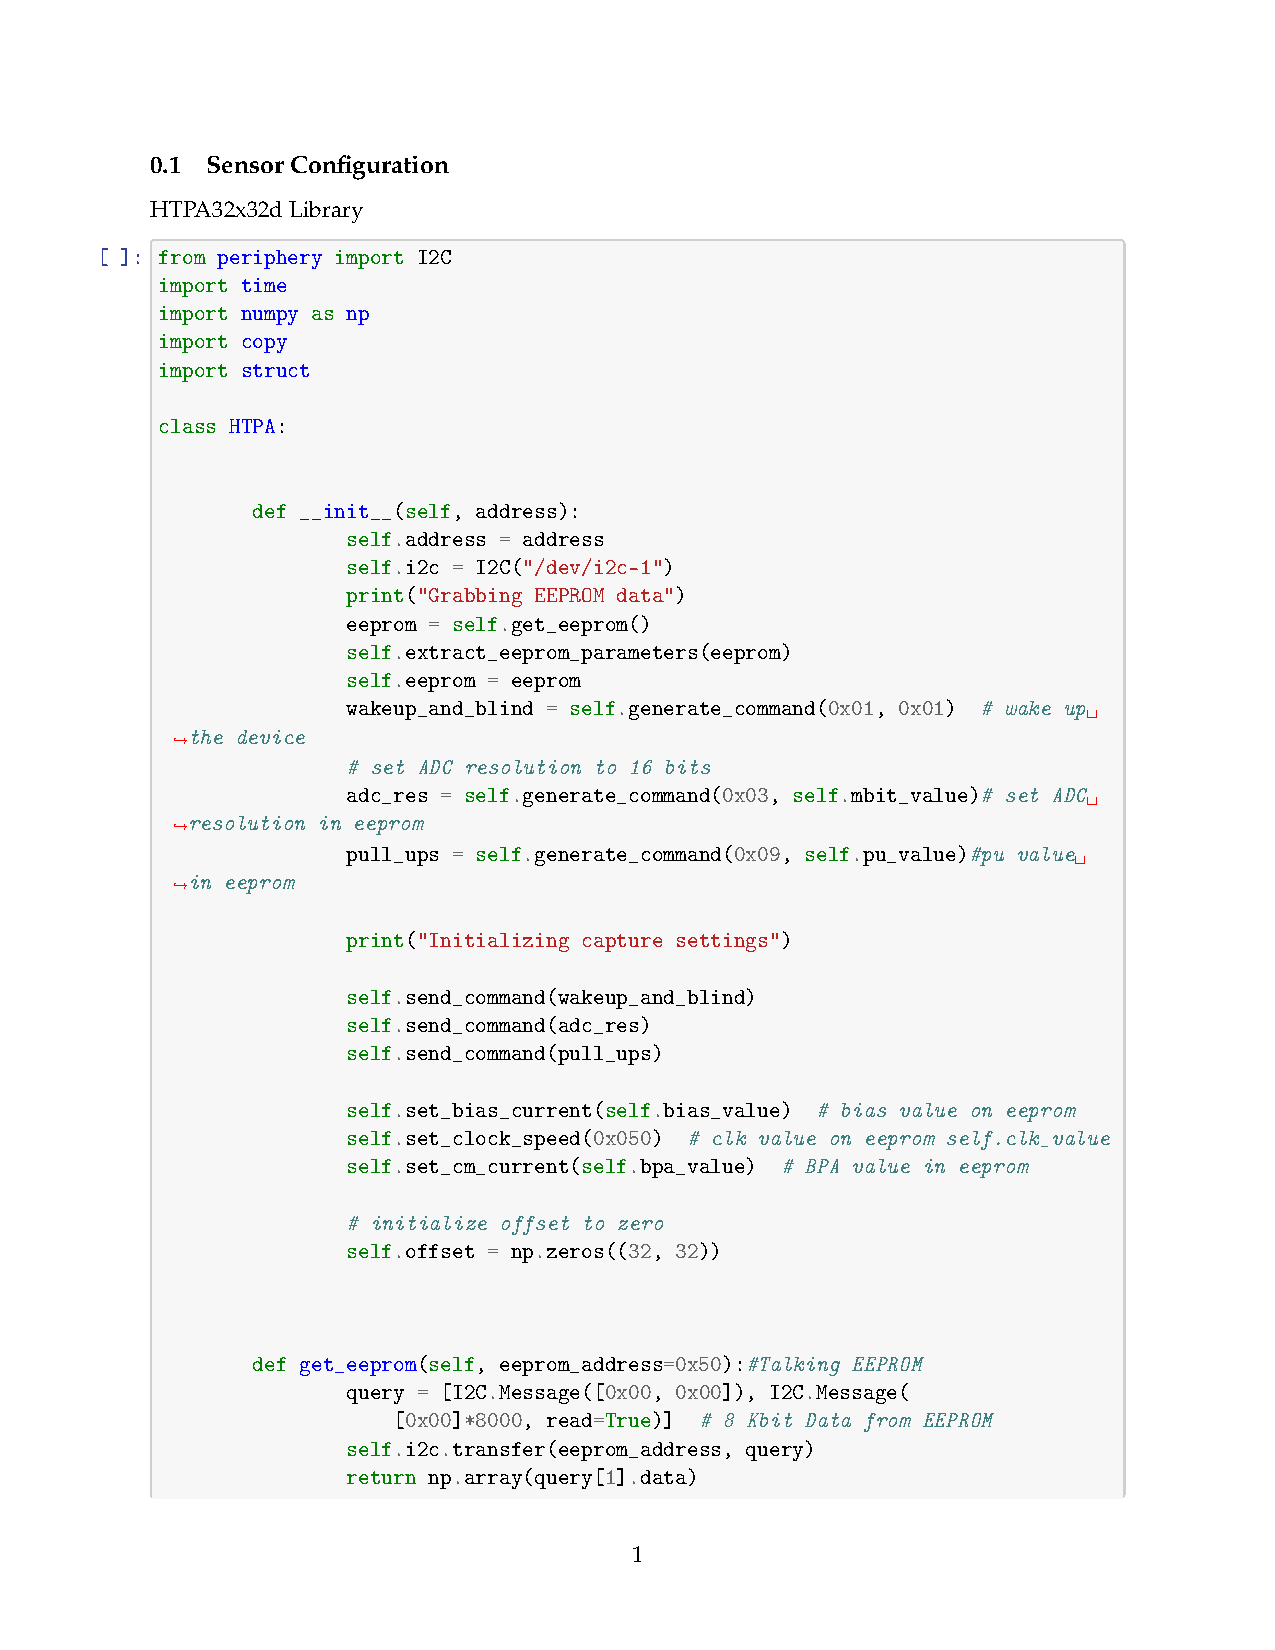
\includepdf[pages=-]{learn.pdf}
	
\end{document}